\documentclass[]{book}
\usepackage{lmodern}
\usepackage{amssymb,amsmath}
\usepackage{ifxetex,ifluatex}
\usepackage{fixltx2e} % provides \textsubscript
\ifnum 0\ifxetex 1\fi\ifluatex 1\fi=0 % if pdftex
  \usepackage[T1]{fontenc}
  \usepackage[utf8]{inputenc}
\else % if luatex or xelatex
  \ifxetex
    \usepackage{mathspec}
  \else
    \usepackage{fontspec}
  \fi
  \defaultfontfeatures{Ligatures=TeX,Scale=MatchLowercase}
\fi
% use upquote if available, for straight quotes in verbatim environments
\IfFileExists{upquote.sty}{\usepackage{upquote}}{}
% use microtype if available
\IfFileExists{microtype.sty}{%
\usepackage{microtype}
\UseMicrotypeSet[protrusion]{basicmath} % disable protrusion for tt fonts
}{}
\usepackage[margin=1in]{geometry}
\usepackage{hyperref}
\hypersetup{unicode=true,
            pdftitle={Data Science for Biological, Medical and Health Research: Notes for 432},
            pdfauthor={Thomas E. Love, Ph.D.},
            pdfborder={0 0 0},
            breaklinks=true}
\urlstyle{same}  % don't use monospace font for urls
\usepackage{natbib}
\bibliographystyle{apalike}
\usepackage{color}
\usepackage{fancyvrb}
\newcommand{\VerbBar}{|}
\newcommand{\VERB}{\Verb[commandchars=\\\{\}]}
\DefineVerbatimEnvironment{Highlighting}{Verbatim}{commandchars=\\\{\}}
% Add ',fontsize=\small' for more characters per line
\usepackage{framed}
\definecolor{shadecolor}{RGB}{248,248,248}
\newenvironment{Shaded}{\begin{snugshade}}{\end{snugshade}}
\newcommand{\KeywordTok}[1]{\textcolor[rgb]{0.13,0.29,0.53}{\textbf{#1}}}
\newcommand{\DataTypeTok}[1]{\textcolor[rgb]{0.13,0.29,0.53}{#1}}
\newcommand{\DecValTok}[1]{\textcolor[rgb]{0.00,0.00,0.81}{#1}}
\newcommand{\BaseNTok}[1]{\textcolor[rgb]{0.00,0.00,0.81}{#1}}
\newcommand{\FloatTok}[1]{\textcolor[rgb]{0.00,0.00,0.81}{#1}}
\newcommand{\ConstantTok}[1]{\textcolor[rgb]{0.00,0.00,0.00}{#1}}
\newcommand{\CharTok}[1]{\textcolor[rgb]{0.31,0.60,0.02}{#1}}
\newcommand{\SpecialCharTok}[1]{\textcolor[rgb]{0.00,0.00,0.00}{#1}}
\newcommand{\StringTok}[1]{\textcolor[rgb]{0.31,0.60,0.02}{#1}}
\newcommand{\VerbatimStringTok}[1]{\textcolor[rgb]{0.31,0.60,0.02}{#1}}
\newcommand{\SpecialStringTok}[1]{\textcolor[rgb]{0.31,0.60,0.02}{#1}}
\newcommand{\ImportTok}[1]{#1}
\newcommand{\CommentTok}[1]{\textcolor[rgb]{0.56,0.35,0.01}{\textit{#1}}}
\newcommand{\DocumentationTok}[1]{\textcolor[rgb]{0.56,0.35,0.01}{\textbf{\textit{#1}}}}
\newcommand{\AnnotationTok}[1]{\textcolor[rgb]{0.56,0.35,0.01}{\textbf{\textit{#1}}}}
\newcommand{\CommentVarTok}[1]{\textcolor[rgb]{0.56,0.35,0.01}{\textbf{\textit{#1}}}}
\newcommand{\OtherTok}[1]{\textcolor[rgb]{0.56,0.35,0.01}{#1}}
\newcommand{\FunctionTok}[1]{\textcolor[rgb]{0.00,0.00,0.00}{#1}}
\newcommand{\VariableTok}[1]{\textcolor[rgb]{0.00,0.00,0.00}{#1}}
\newcommand{\ControlFlowTok}[1]{\textcolor[rgb]{0.13,0.29,0.53}{\textbf{#1}}}
\newcommand{\OperatorTok}[1]{\textcolor[rgb]{0.81,0.36,0.00}{\textbf{#1}}}
\newcommand{\BuiltInTok}[1]{#1}
\newcommand{\ExtensionTok}[1]{#1}
\newcommand{\PreprocessorTok}[1]{\textcolor[rgb]{0.56,0.35,0.01}{\textit{#1}}}
\newcommand{\AttributeTok}[1]{\textcolor[rgb]{0.77,0.63,0.00}{#1}}
\newcommand{\RegionMarkerTok}[1]{#1}
\newcommand{\InformationTok}[1]{\textcolor[rgb]{0.56,0.35,0.01}{\textbf{\textit{#1}}}}
\newcommand{\WarningTok}[1]{\textcolor[rgb]{0.56,0.35,0.01}{\textbf{\textit{#1}}}}
\newcommand{\AlertTok}[1]{\textcolor[rgb]{0.94,0.16,0.16}{#1}}
\newcommand{\ErrorTok}[1]{\textcolor[rgb]{0.64,0.00,0.00}{\textbf{#1}}}
\newcommand{\NormalTok}[1]{#1}
\usepackage{longtable,booktabs}
\usepackage{graphicx,grffile}
\makeatletter
\def\maxwidth{\ifdim\Gin@nat@width>\linewidth\linewidth\else\Gin@nat@width\fi}
\def\maxheight{\ifdim\Gin@nat@height>\textheight\textheight\else\Gin@nat@height\fi}
\makeatother
% Scale images if necessary, so that they will not overflow the page
% margins by default, and it is still possible to overwrite the defaults
% using explicit options in \includegraphics[width, height, ...]{}
\setkeys{Gin}{width=\maxwidth,height=\maxheight,keepaspectratio}
\IfFileExists{parskip.sty}{%
\usepackage{parskip}
}{% else
\setlength{\parindent}{0pt}
\setlength{\parskip}{6pt plus 2pt minus 1pt}
}
\setlength{\emergencystretch}{3em}  % prevent overfull lines
\providecommand{\tightlist}{%
  \setlength{\itemsep}{0pt}\setlength{\parskip}{0pt}}
\setcounter{secnumdepth}{5}
% Redefines (sub)paragraphs to behave more like sections
\ifx\paragraph\undefined\else
\let\oldparagraph\paragraph
\renewcommand{\paragraph}[1]{\oldparagraph{#1}\mbox{}}
\fi
\ifx\subparagraph\undefined\else
\let\oldsubparagraph\subparagraph
\renewcommand{\subparagraph}[1]{\oldsubparagraph{#1}\mbox{}}
\fi

%%% Use protect on footnotes to avoid problems with footnotes in titles
\let\rmarkdownfootnote\footnote%
\def\footnote{\protect\rmarkdownfootnote}

%%% Change title format to be more compact
\usepackage{titling}

% Create subtitle command for use in maketitle
\newcommand{\subtitle}[1]{
  \posttitle{
    \begin{center}\large#1\end{center}
    }
}

\setlength{\droptitle}{-2em}
  \title{Data Science for Biological, Medical and Health Research: Notes for 432}
  \pretitle{\vspace{\droptitle}\centering\huge}
  \posttitle{\par}
  \author{Thomas E. Love, Ph.D.}
  \preauthor{\centering\large\emph}
  \postauthor{\par}
  \predate{\centering\large\emph}
  \postdate{\par}
  \date{Built 2018-01-21 13:21:38}

\usepackage{booktabs}
\usepackage{amsthm}
\makeatletter
\def\thm@space@setup{%
  \thm@preskip=8pt plus 2pt minus 4pt
  \thm@postskip=\thm@preskip
}
\makeatother

\usepackage{amsthm}
\newtheorem{theorem}{Theorem}[chapter]
\newtheorem{lemma}{Lemma}[chapter]
\theoremstyle{definition}
\newtheorem{definition}{Definition}[chapter]
\newtheorem{corollary}{Corollary}[chapter]
\newtheorem{proposition}{Proposition}[chapter]
\theoremstyle{definition}
\newtheorem{example}{Example}[chapter]
\theoremstyle{definition}
\newtheorem{exercise}{Exercise}[chapter]
\theoremstyle{remark}
\newtheorem*{remark}{Remark}
\newtheorem*{solution}{Solution}
\begin{document}
\maketitle

{
\setcounter{tocdepth}{1}
\tableofcontents
}
\chapter*{Introduction}\label{introduction}
\addcontentsline{toc}{chapter}{Introduction}

These Notes provide a series of examples using R to work through issues
that are likely to come up in PQHS/CRSP/MPHP 432.

While these Notes share some of the features of a textbook, they are
neither comprehensive nor completely original. The main purpose is to
give students in 432 a set of common materials on which to draw during
the course. In class, we will sometimes:

\begin{itemize}
\tightlist
\item
  reiterate points made in this document,
\item
  amplify what is here,
\item
  simplify the presentation of things done here,
\item
  use new examples to show some of the same techniques,
\item
  refer to issues not mentioned in this document,
\end{itemize}

but what we don't (always) do is follow these notes very precisely. We
assume instead that you will read the materials and try to learn from
them, just as you will attend classes and try to learn from them. We
welcome feedback of all kinds on this document or anything else. Just
email us at \texttt{431-help\ at\ case\ dot\ edu}, or submit a pull
request. Note that we still use \texttt{431-help} even though we're now
in 432.

What you will mostly find are brief explanations of a key idea or
summary, accompanied (most of the time) by R code and a demonstration of
the results of applying that code.

Everything you see here is available to you as HTML or PDF. You will
also have access to the R Markdown files, which contain the code which
generates everything in the document, including all of the R results. We
will demonstrate the use of R Markdown (this document is generated with
the additional help of an R package called bookdown) and R Studio (the
``program'' which we use to interface with the R language) in class.

To download the data and R code related to these notes, visit the Data
and Code section of \href{https://github.com/THOMASELOVE/432-2018}{the
432 course website}.

\chapter*{R Packages used in these
notes}\label{r-packages-used-in-these-notes}
\addcontentsline{toc}{chapter}{R Packages used in these notes}

Here, we'll load in the packages used in these notes.

\begin{Shaded}
\begin{Highlighting}[]
\KeywordTok{library}\NormalTok{(tableone)}
\KeywordTok{library}\NormalTok{(skimr)}
\KeywordTok{library}\NormalTok{(simputation)}
\KeywordTok{library}\NormalTok{(magrittr)}
\KeywordTok{library}\NormalTok{(modelr)}
\KeywordTok{library}\NormalTok{(broom)}
\KeywordTok{library}\NormalTok{(tidyverse)}
\end{Highlighting}
\end{Shaded}

\chapter*{Data used in these notes}\label{data-used-in-these-notes}
\addcontentsline{toc}{chapter}{Data used in these notes}

Here, we'll load in the data sets used in these notes.

\begin{Shaded}
\begin{Highlighting}[]
\NormalTok{fakestroke <-}\StringTok{ }\KeywordTok{read.csv}\NormalTok{(}\StringTok{"data/fakestroke.csv"}\NormalTok{) }\OperatorTok\StringTok{ }\NormalTok{tbl_df}
\NormalTok{bloodbrain <-}\StringTok{ }\KeywordTok{read.csv}\NormalTok{(}\StringTok{"data/bloodbrain.csv"}\NormalTok{) }\OperatorTok\StringTok{ }\NormalTok{tbl_df}
\NormalTok{smartcle1 <-}\StringTok{ }\KeywordTok{read.csv}\NormalTok{(}\StringTok{"data/smartcle1.csv"}\NormalTok{) }\OperatorTok\StringTok{ }\NormalTok{tbl_df}
\NormalTok{bonding <-}\StringTok{ }\KeywordTok{read.csv}\NormalTok{(}\StringTok{"data/bonding.csv"}\NormalTok{) }\OperatorTok\StringTok{ }\NormalTok{tbl_df}
\NormalTok{cortisol <-}\StringTok{ }\KeywordTok{read.csv}\NormalTok{(}\StringTok{"data/cortisol.csv"}\NormalTok{) }\OperatorTok\StringTok{ }\NormalTok{tbl_df}
\end{Highlighting}
\end{Shaded}

\chapter{Building Table 1}\label{building-table-1}

Many scientific articles involve direct comparison of results from
various exposures, perhaps treatments. In 431, we studied numerous
methods, including various sorts of hypothesis tests, confidence
intervals, and descriptive summaries, which can help us to understand
and compare outcomes in such a setting. One common approach is to
present what's often called Table 1. Table 1 provides a summary of the
characteristics of a sample, or of groups of samples, which is most
commonly used to help understand the nature of the data being compared.

\section{\texorpdfstring{Two examples from the \emph{New England Journal
of
Medicine}}{Two examples from the New England Journal of Medicine}}\label{two-examples-from-the-new-england-journal-of-medicine}

\subsection{A simple Table 1}\label{a-simple-table-1}

Table 1 is especially common in the context of clinical research.
Consider the excerpt below, from a January 2015 article in the \emph{New
England Journal of Medicine} \citep{Tolaney2015}.

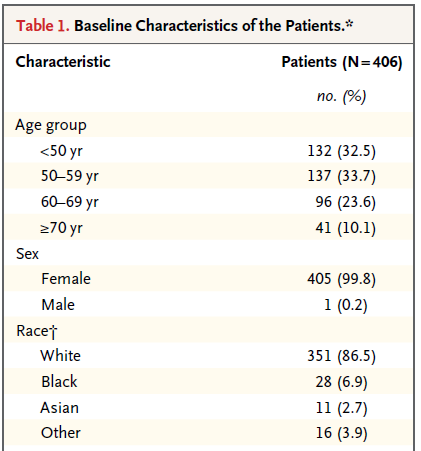
\includegraphics[width=0.5\linewidth]{images/Tolaney-snip1}

This (partial) table reports baseline characteristics on age group, sex
and race, describing 406 patients with HER2-positive\footnote{HER2 =
  human epidermal growth factor receptor type 2. Over-expression of this
  occurs in 15-20\% of invasive breast cancers, and has been associated
  with poor outcomes.} invasive breast cancer that began the protocol
therapy. Age, sex and race (along with severity of illness) are the most
commonly identified characteristics in a Table 1.

In addition to the measures shown in this excerpt, the full Table also
includes detailed information on the primary tumor for each patient,
including its size, nodal status and histologic grade. Footnotes tell us
that the percentages shown are subject to rounding, and may not total
100, and that the race information was self-reported.

\subsection{A group comparison}\label{a-group-comparison}

A more typical Table 1 involves a group comparison, for example in this
excerpt from \citet{Roy2008}. This Table 1 describes a multi-center
randomized clinical trial comparing two different approaches to caring
for patients with heart failure and atrial fibrillation\footnote{The
  complete Table 1 appears on pages 2668-2669 of \citet{Roy2008}, but I
  have only reproduced the first page and the footnote in this excerpt.}.

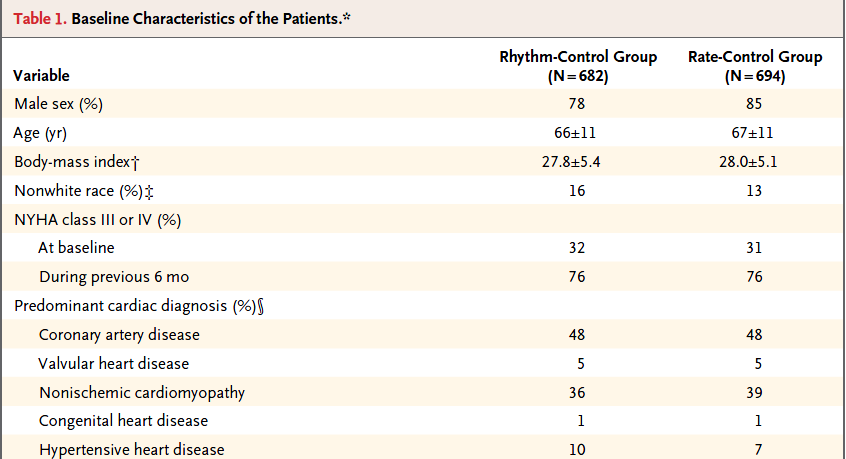
\includegraphics[width=0.9\linewidth]{images/Roy-snip1}

The article provides percentages, means and standard deviations across
groups, but note that it does not provide p values for the comparison of
baseline characteristics. This is a common feature of NEJM reports on
randomized clinical trials, where we anticipate that the two groups will
be well matched at baseline. Note that the patients in this study were
\emph{randomly} assigned to either the rhythm-control group or to the
rate-control group, using blocked randomizations stratified by study
center.

\section{The MR CLEAN trial}\label{the-mr-clean-trial}

\citet{Berkhemer2015} reported on the MR CLEAN trial, involving 500
patients with acute ischemic stroke caused by a proximal intracranial
arterial occlusion. The trial was conducted at 16 medical centers in the
Netherlands, where 233 were randomly assigned to the intervention
(intraarterial treatment plus usual care) and 267 to control (usual care
alone.) The primary outcome was the modified Rankin scale score at 90
days; this categorical scale measures functional outcome, with scores
ranging from 0 (no symptoms) to 6 (death). The fundamental conclusion of
\citet{Berkhemer2015} was that in patients with acute ischemic stroke
caused by a proximal intracranial occlusion of the anterior circulation,
intraarterial treatment administered within 6 hours after stroke onset
was effective and safe.

Here's the Table 1 from \citet{Berkhemer2015}.

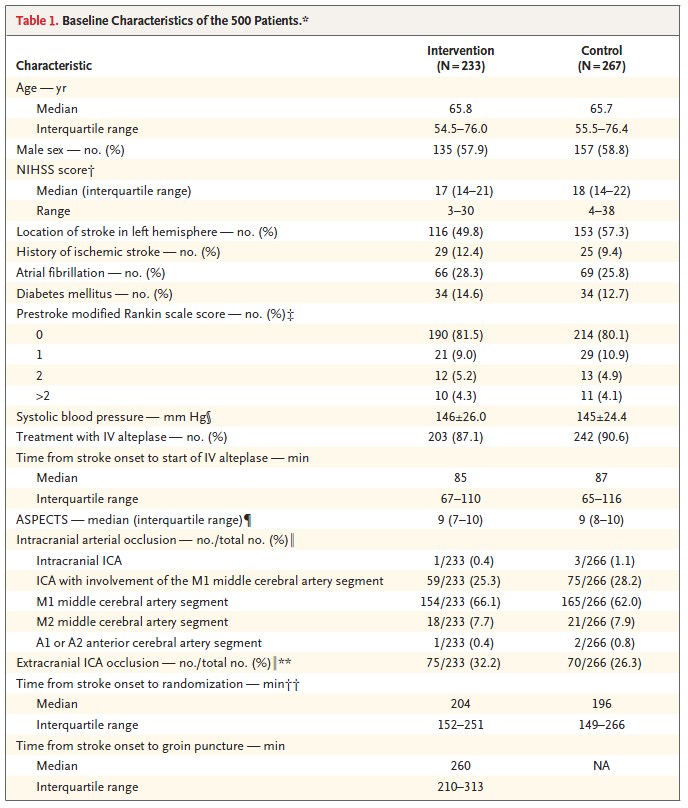
\includegraphics[width=0.9\linewidth]{images/Berkhemer-snip4complete}

The Table was accompanied by the following notes.

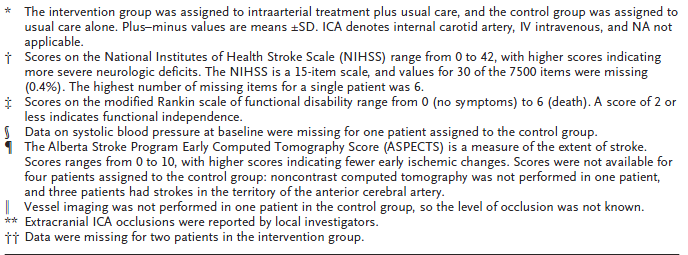
\includegraphics[width=0.9\linewidth]{images/Berkhemer-snip4notes}

\section{\texorpdfstring{Simulated \texttt{fakestroke}
data}{Simulated fakestroke data}}\label{simulated-fakestroke-data}

Consider the simulated data, available on the Data and Code page of
\href{https://github.com/THOMASELOVE/432-2018}{our course website} in
the \texttt{fakestroke.csv} file, which I built to let us mirror the
Table 1 for MR CLEAN \citep{Berkhemer2015}. The \texttt{fakestroke.csv}
file contains the following 18 variables for 500 patients.

\begin{longtable}[]{@{}rl@{}}
\toprule
\begin{minipage}[b]{0.16\columnwidth}\raggedleft\strut
Variable\strut
\end{minipage} & \begin{minipage}[b]{0.55\columnwidth}\raggedright\strut
Description\strut
\end{minipage}\tabularnewline
\midrule
\endhead
\begin{minipage}[t]{0.16\columnwidth}\raggedleft\strut
\texttt{studyid}\strut
\end{minipage} & \begin{minipage}[t]{0.55\columnwidth}\raggedright\strut
Study ID \# (z001 through z500)\strut
\end{minipage}\tabularnewline
\begin{minipage}[t]{0.16\columnwidth}\raggedleft\strut
\texttt{trt}\strut
\end{minipage} & \begin{minipage}[t]{0.55\columnwidth}\raggedright\strut
Treatment group (Intervention or Control)\strut
\end{minipage}\tabularnewline
\begin{minipage}[t]{0.16\columnwidth}\raggedleft\strut
\texttt{age}\strut
\end{minipage} & \begin{minipage}[t]{0.55\columnwidth}\raggedright\strut
Age in years\strut
\end{minipage}\tabularnewline
\begin{minipage}[t]{0.16\columnwidth}\raggedleft\strut
\texttt{sex}\strut
\end{minipage} & \begin{minipage}[t]{0.55\columnwidth}\raggedright\strut
Male or Female\strut
\end{minipage}\tabularnewline
\begin{minipage}[t]{0.16\columnwidth}\raggedleft\strut
\texttt{nihss}\strut
\end{minipage} & \begin{minipage}[t]{0.55\columnwidth}\raggedright\strut
NIH Stroke Scale Score (can range from 0-42; higher scores indicate more
severe neurological deficits)\strut
\end{minipage}\tabularnewline
\begin{minipage}[t]{0.16\columnwidth}\raggedleft\strut
\texttt{location}\strut
\end{minipage} & \begin{minipage}[t]{0.55\columnwidth}\raggedright\strut
Stroke Location - Left or Right Hemisphere\strut
\end{minipage}\tabularnewline
\begin{minipage}[t]{0.16\columnwidth}\raggedleft\strut
\texttt{hx.isch}\strut
\end{minipage} & \begin{minipage}[t]{0.55\columnwidth}\raggedright\strut
History of Ischemic Stroke (Yes/No)\strut
\end{minipage}\tabularnewline
\begin{minipage}[t]{0.16\columnwidth}\raggedleft\strut
\texttt{afib}\strut
\end{minipage} & \begin{minipage}[t]{0.55\columnwidth}\raggedright\strut
Atrial Fibrillation (1 = Yes, 0 = No)\strut
\end{minipage}\tabularnewline
\begin{minipage}[t]{0.16\columnwidth}\raggedleft\strut
\texttt{dm}\strut
\end{minipage} & \begin{minipage}[t]{0.55\columnwidth}\raggedright\strut
Diabetes Mellitus (1 = Yes, 0 = No)\strut
\end{minipage}\tabularnewline
\begin{minipage}[t]{0.16\columnwidth}\raggedleft\strut
\texttt{mrankin}\strut
\end{minipage} & \begin{minipage}[t]{0.55\columnwidth}\raggedright\strut
Pre-stroke modified Rankin scale score (0, 1, 2 or \textgreater{} 2)
indicating functional disability - complete range is 0 (no symptoms) to
6 (death)\strut
\end{minipage}\tabularnewline
\begin{minipage}[t]{0.16\columnwidth}\raggedleft\strut
\texttt{sbp}\strut
\end{minipage} & \begin{minipage}[t]{0.55\columnwidth}\raggedright\strut
Systolic blood pressure, in mm Hg\strut
\end{minipage}\tabularnewline
\begin{minipage}[t]{0.16\columnwidth}\raggedleft\strut
\texttt{iv.altep}\strut
\end{minipage} & \begin{minipage}[t]{0.55\columnwidth}\raggedright\strut
Treatment with IV alteplase (Yes/No)\strut
\end{minipage}\tabularnewline
\begin{minipage}[t]{0.16\columnwidth}\raggedleft\strut
\texttt{time.iv}\strut
\end{minipage} & \begin{minipage}[t]{0.55\columnwidth}\raggedright\strut
Time from stroke onset to start of IV alteplase (minutes) if
iv.altep=Yes\strut
\end{minipage}\tabularnewline
\begin{minipage}[t]{0.16\columnwidth}\raggedleft\strut
\texttt{aspects}\strut
\end{minipage} & \begin{minipage}[t]{0.55\columnwidth}\raggedright\strut
Alberta Stroke Program Early Computed Tomography score, which measures
extent of stroke from 0 - 10; higher scores indicate fewer early
ischemic changes\strut
\end{minipage}\tabularnewline
\begin{minipage}[t]{0.16\columnwidth}\raggedleft\strut
\texttt{ia.occlus}\strut
\end{minipage} & \begin{minipage}[t]{0.55\columnwidth}\raggedright\strut
Intracranial arterial occlusion, based on vessel imaging - five
categories\footnotemark{}\strut
\end{minipage}
\footnotetext{The five categories are Intracranial ICA, ICA with
  involvement of the M1 middle cerebral artery segment, M1 middle
  cerebral artery segment, M2 middle cerebral artery segment, A1 or A2
  anterior cerebral artery segment}\tabularnewline
\begin{minipage}[t]{0.16\columnwidth}\raggedleft\strut
\texttt{extra.ica}\strut
\end{minipage} & \begin{minipage}[t]{0.55\columnwidth}\raggedright\strut
Extracranial ICA occlusion (1 = Yes, 0 = No)\strut
\end{minipage}\tabularnewline
\begin{minipage}[t]{0.16\columnwidth}\raggedleft\strut
\texttt{time.rand}\strut
\end{minipage} & \begin{minipage}[t]{0.55\columnwidth}\raggedright\strut
Time from stroke onset to study randomization, in minutes\strut
\end{minipage}\tabularnewline
\begin{minipage}[t]{0.16\columnwidth}\raggedleft\strut
\texttt{time.punc}\strut
\end{minipage} & \begin{minipage}[t]{0.55\columnwidth}\raggedright\strut
Time from stroke onset to groin puncture, in minutes (only if
Intervention)\strut
\end{minipage}\tabularnewline
\bottomrule
\end{longtable}

Here's a quick look at the simulated data in \texttt{fakestroke}.

\begin{Shaded}
\begin{Highlighting}[]
\NormalTok{fakestroke}
\end{Highlighting}
\end{Shaded}

\begin{verbatim}
# A tibble: 500 x 18
   studyid trt        age sex   nihss location hx.isch  afib    dm mrankin
   <fct>   <fct>    <dbl> <fct> <int> <fct>    <fct>   <int> <int> <fct>  
 1 z001    Control   53.0 Male     21 Right    No          0     0 2      
 2 z002    Interve~  51.0 Male     23 Left     No          1     0 0      
 3 z003    Control   68.0 Fema~    11 Right    No          0     0 0      
 4 z004    Control   28.0 Male     22 Left     No          0     0 0      
 5 z005    Control   91.0 Male     24 Right    No          0     0 0      
 6 z006    Control   34.0 Fema~    18 Left     No          0     0 2      
 7 z007    Interve~  75.0 Male     25 Right    No          0     0 0      
 8 z008    Control   89.0 Fema~    18 Right    No          0     0 0      
 9 z009    Control   75.0 Male     25 Left     No          1     0 2      
10 z010    Interve~  26.0 Fema~    27 Right    No          0     0 0      
# ... with 490 more rows, and 8 more variables: sbp <int>, iv.altep <fct>,
#   time.iv <int>, aspects <int>, ia.occlus <fct>, extra.ica <int>,
#   time.rand <int>, time.punc <int>
\end{verbatim}

\section{\texorpdfstring{Building Table 1 for \texttt{fakestroke}:
Attempt
1}{Building Table 1 for fakestroke: Attempt 1}}\label{building-table-1-for-fakestroke-attempt-1}

Our goal, then, is to take the data in \texttt{fakestroke.csv} and use
it to generate a Table 1 for the study that compares the 233 patients in
the Intervention group to the 267 patients in the Control group, on all
of the other variables (except study ID \#) available. I'll use the
\texttt{tableone} package of functions available in R to help me
complete this task. We'll make a first attempt, using the
\texttt{CreateTableOne} function in the \texttt{tableone} package. To
use the function, we'll need to specify:

\begin{itemize}
\tightlist
\item
  the \texttt{vars} or variables we want to place in the rows of our
  Table 1 (which will include just about everything in the
  \texttt{fakestroke} data except the \texttt{studyid} code and the
  \texttt{trt} variable for which we have other plans, and the
  \texttt{time.punc} which applies only to subjects in the Intervention
  group.)

  \begin{itemize}
  \tightlist
  \item
    A useful trick here is to use the \texttt{dput} function,
    specifically something like \texttt{dput(names(fakestroke))} can be
    used to generate a list of all of the variables included in the
    \texttt{fakestroke} tibble, and then this can be copied and pasted
    into the \texttt{vars} specification, saving some typing.
  \end{itemize}
\item
  the \texttt{strata} which indicates the levels want to use in the
  columns of our Table 1 (for us, that's \texttt{trt})
\end{itemize}

\begin{Shaded}
\begin{Highlighting}[]
\NormalTok{fs.vars <-}\StringTok{ }\KeywordTok{c}\NormalTok{(}\StringTok{"age"}\NormalTok{, }\StringTok{"sex"}\NormalTok{, }\StringTok{"nihss"}\NormalTok{, }\StringTok{"location"}\NormalTok{, }
          \StringTok{"hx.isch"}\NormalTok{, }\StringTok{"afib"}\NormalTok{, }\StringTok{"dm"}\NormalTok{, }\StringTok{"mrankin"}\NormalTok{, }\StringTok{"sbp"}\NormalTok{,}
          \StringTok{"iv.altep"}\NormalTok{, }\StringTok{"time.iv"}\NormalTok{, }\StringTok{"aspects"}\NormalTok{, }
          \StringTok{"ia.occlus"}\NormalTok{, }\StringTok{"extra.ica"}\NormalTok{, }\StringTok{"time.rand"}\NormalTok{)}

\NormalTok{fs.trt <-}\StringTok{ }\KeywordTok{c}\NormalTok{(}\StringTok{"trt"}\NormalTok{)}

\NormalTok{att1 <-}\StringTok{ }\KeywordTok{CreateTableOne}\NormalTok{(}\DataTypeTok{data =}\NormalTok{ fakestroke, }
                       \DataTypeTok{vars =}\NormalTok{ fs.vars, }
                       \DataTypeTok{strata =}\NormalTok{ fs.trt)}
\KeywordTok{print}\NormalTok{(att1)}
\end{Highlighting}
\end{Shaded}

\begin{verbatim}
                       Stratified by trt
                        Control        Intervention   p      test
  n                        267            233                    
  age (mean (sd))        65.38 (16.10)  63.93 (18.09)  0.343     
  sex = Male (%)           157 (58.8)     135 (57.9)   0.917     
  nihss (mean (sd))      18.08 (4.32)   17.97 (5.04)   0.787     
  location = Right (%)     114 (42.7)     117 (50.2)   0.111     
  hx.isch = Yes (%)         25 ( 9.4)      29 (12.4)   0.335     
  afib (mean (sd))        0.26 (0.44)    0.28 (0.45)   0.534     
  dm (mean (sd))          0.13 (0.33)    0.12 (0.33)   0.923     
  mrankin (%)                                          0.922     
     > 2                    11 ( 4.1)      10 ( 4.3)             
     0                     214 (80.1)     190 (81.5)             
     1                      29 (10.9)      21 ( 9.0)             
     2                      13 ( 4.9)      12 ( 5.2)             
  sbp (mean (sd))       145.00 (24.40) 146.03 (26.00)  0.647     
  iv.altep = Yes (%)       242 (90.6)     203 (87.1)   0.267     
  time.iv (mean (sd))    87.96 (26.01)  98.22 (45.48)  0.003     
  aspects (mean (sd))     8.65 (1.47)    8.35 (1.64)   0.033     
  ia.occlus (%)                                        0.795     
     A1 or A2                2 ( 0.8)       1 ( 0.4)             
     ICA with M1            75 (28.2)      59 (25.3)             
     Intracranial ICA        3 ( 1.1)       1 ( 0.4)             
     M1                    165 (62.0)     154 (66.1)             
     M2                     21 ( 7.9)      18 ( 7.7)             
  extra.ica (mean (sd))   0.26 (0.44)    0.32 (0.47)   0.150     
  time.rand (mean (sd)) 213.88 (70.29) 202.51 (57.33)  0.051     
\end{verbatim}

\subsection{Some of this is very useful, and other parts need to be
fixed.}\label{some-of-this-is-very-useful-and-other-parts-need-to-be-fixed.}

\begin{enumerate}
\def\labelenumi{\arabic{enumi}.}
\tightlist
\item
  The 1/0 variables (\texttt{afib}, \texttt{dm}, \texttt{extra.ica})
  might be better if they were treated as the factors they are, and
  reported as the Yes/No variables are reported, with counts and
  percentages rather than with means and standard deviations.
\item
  In some cases, we may prefer to re-order the levels of the categorical
  (factor) variables, particularly the \texttt{mrankin} variable, but
  also the \texttt{ia.occlus} variable. It would also be more typical to
  put the Intervention group to the left and the Control group to the
  right, so we may need to adjust our \texttt{trt} variable's levels
  accordingly.
\item
  For each of the quantitative variables (\texttt{age}, \texttt{nihss},
  \texttt{sbp}, \texttt{time.iv}, \texttt{aspects}, \texttt{extra.ica},
  \texttt{time.rand} and \texttt{time.punc}) we should make a decision
  whether a summary with mean and standard deviation is appropriate, or
  whether we should instead summarize with, say, the median and
  quartiles. A mean and standard deviation really only yields an
  appropriate summary when the data are least approximately Normally
  distributed. This will make the \emph{p} values a bit more reasonable,
  too. The \texttt{test} column in the first attempt will soon have
  something useful to tell us.
\item
  If we'd left in the \texttt{time.punc} variable, we'd get some
  warnings, having to do with the fact that \texttt{time.punc} is only
  relevant to patients in the Intervention group.
\end{enumerate}

\subsection{\texorpdfstring{\texttt{fakestroke} Cleaning Up Categorical
Variables}{fakestroke Cleaning Up Categorical Variables}}\label{fakestroke-cleaning-up-categorical-variables}

Let's specify each of the categorical variables as categorical
explicitly. This helps the \texttt{CreateTableOne} function treat them
appropriately, and display them with counts and percentages. This
includes all of the 1/0, Yes/No and multi-categorical variables.

\begin{Shaded}
\begin{Highlighting}[]
\NormalTok{fs.factorvars <-}\StringTok{ }\KeywordTok{c}\NormalTok{(}\StringTok{"sex"}\NormalTok{, }\StringTok{"location"}\NormalTok{, }\StringTok{"hx.isch"}\NormalTok{, }\StringTok{"afib"}\NormalTok{, }\StringTok{"dm"}\NormalTok{, }
                   \StringTok{"mrankin"}\NormalTok{, }\StringTok{"iv.altep"}\NormalTok{, }\StringTok{"ia.occlus"}\NormalTok{, }\StringTok{"extra.ica"}\NormalTok{)}
\end{Highlighting}
\end{Shaded}

Then we simply add a \texttt{factorVars\ =\ fs.factorvars} call to the
\texttt{CreateTableOne} function.

We also want to re-order some of those categorical variables, so that
the levels are more useful to us. Specifically, we want to:

\begin{itemize}
\tightlist
\item
  place Intervention before Control in the \texttt{trt} variable,
\item
  reorder the \texttt{mrankin} scale as 0, 1, 2, \textgreater{} 2, and
\item
  rearrange the \texttt{ia.occlus} variable to the order\footnote{We
    might also have considered reordering the \texttt{ia.occlus} factor
    by its frequency, using the \texttt{fct\_infreq} function} presented
  in \citet{Berkhemer2015}.
\end{itemize}

To accomplish this, we'll use the \texttt{fct\_relevel} function from
the \texttt{forcats} package (loaded with the rest of the core
\texttt{tidyverse} packages) to reorder our levels manually.

\begin{Shaded}
\begin{Highlighting}[]
\NormalTok{fakestroke <-}\StringTok{ }\NormalTok{fakestroke }\OperatorTok
\StringTok{    }\KeywordTok{mutate}\NormalTok{(}\DataTypeTok{trt =} \KeywordTok{fct_relevel}\NormalTok{(trt, }\StringTok{"Intervention"}\NormalTok{, }\StringTok{"Control"}\NormalTok{),}
           \DataTypeTok{mrankin =} \KeywordTok{fct_relevel}\NormalTok{(mrankin, }\StringTok{"0"}\NormalTok{, }\StringTok{"1"}\NormalTok{, }\StringTok{"2"}\NormalTok{, }\StringTok{"> 2"}\NormalTok{),}
           \DataTypeTok{ia.occlus =} \KeywordTok{fct_relevel}\NormalTok{(ia.occlus, }\StringTok{"Intracranial ICA"}\NormalTok{, }
                                   \StringTok{"ICA with M1"}\NormalTok{, }\StringTok{"M1"}\NormalTok{, }\StringTok{"M2"}\NormalTok{, }
                                   \StringTok{"A1 or A2"}\NormalTok{)}
\NormalTok{           ) }
\end{Highlighting}
\end{Shaded}

\section{\texorpdfstring{\texttt{fakestroke} Table 1: Attempt
2}{fakestroke Table 1: Attempt 2}}\label{fakestroke-table-1-attempt-2}

\begin{Shaded}
\begin{Highlighting}[]
\NormalTok{att2 <-}\StringTok{ }\KeywordTok{CreateTableOne}\NormalTok{(}\DataTypeTok{data =}\NormalTok{ fakestroke, }
                       \DataTypeTok{vars =}\NormalTok{ fs.vars,}
                       \DataTypeTok{factorVars =}\NormalTok{ fs.factorvars,}
                       \DataTypeTok{strata =}\NormalTok{ fs.trt)}
\KeywordTok{print}\NormalTok{(att2)}
\end{Highlighting}
\end{Shaded}

\begin{verbatim}
                       Stratified by trt
                        Intervention   Control        p      test
  n                        233            267                    
  age (mean (sd))        63.93 (18.09)  65.38 (16.10)  0.343     
  sex = Male (%)           135 (57.9)     157 (58.8)   0.917     
  nihss (mean (sd))      17.97 (5.04)   18.08 (4.32)   0.787     
  location = Right (%)     117 (50.2)     114 (42.7)   0.111     
  hx.isch = Yes (%)         29 (12.4)      25 ( 9.4)   0.335     
  afib = 1 (%)              66 (28.3)      69 (25.8)   0.601     
  dm = 1 (%)                29 (12.4)      34 (12.7)   1.000     
  mrankin (%)                                          0.922     
     0                     190 (81.5)     214 (80.1)             
     1                      21 ( 9.0)      29 (10.9)             
     2                      12 ( 5.2)      13 ( 4.9)             
     > 2                    10 ( 4.3)      11 ( 4.1)             
  sbp (mean (sd))       146.03 (26.00) 145.00 (24.40)  0.647     
  iv.altep = Yes (%)       203 (87.1)     242 (90.6)   0.267     
  time.iv (mean (sd))    98.22 (45.48)  87.96 (26.01)  0.003     
  aspects (mean (sd))     8.35 (1.64)    8.65 (1.47)   0.033     
  ia.occlus (%)                                        0.795     
     Intracranial ICA        1 ( 0.4)       3 ( 1.1)             
     ICA with M1            59 (25.3)      75 (28.2)             
     M1                    154 (66.1)     165 (62.0)             
     M2                     18 ( 7.7)      21 ( 7.9)             
     A1 or A2                1 ( 0.4)       2 ( 0.8)             
  extra.ica = 1 (%)         75 (32.2)      70 (26.3)   0.179     
  time.rand (mean (sd)) 202.51 (57.33) 213.88 (70.29)  0.051     
\end{verbatim}

The categorical data presentation looks much improved.

\subsection{What summaries should we
show?}\label{what-summaries-should-we-show}

Now, we'll move on to the issue of making a decision about what type of
summary to show for the quantitative variables. Since the
\texttt{fakestroke} data are just simulated and only match the summary
statistics of the original results, not the details, we'll adopt the
decisions made by \citet{Berkhemer2015}, which were to use medians and
interquartile ranges to summarize the distributions of all of the
continuous variables \textbf{except} systolic blood pressure.

\begin{itemize}
\tightlist
\item
  Specifying certain quantitative variables as \emph{non-normal} causes
  R to show them with medians and the 25th and 75th percentiles, rather
  than means and standard deviations, and also causes those variables to
  be tested using non-parametric tests, like the Wilcoxon signed rank
  test, rather than the t test. The \texttt{test} column indicates this
  with the word \texttt{nonnorm}.

  \begin{itemize}
  \tightlist
  \item
    In real data situations, what should we do? The answer is to look at
    the data. I would not make the decision as to which approach to take
    without first plotting (perhaps in a histogram or a Normal Q-Q plot)
    the observed distributions in each of the two samples, so that I
    could make a sound decision about whether Normality was a reasonable
    assumption. If the means and medians are meaningfully different from
    each other, this is especially important.
  \item
    To be honest, though, if the variable in question is a relatively
    unimportant covariate and the \emph{p} values for the two approaches
    are nearly the same, I'm not sure that further investigation is
    especially important,
  \end{itemize}
\item
  Specifying \emph{exact} tests for certain categorical variables (we'll
  try this for the \texttt{location} and \texttt{mrankin} variables) can
  be done, and these changes will be noted in the \texttt{test} column,
  as well.

  \begin{itemize}
  \tightlist
  \item
    In real data situations, I would rarely be concerned about this
    issue, and often choose Pearson (approximate) options across the
    board. This is reasonable so long as the number of subjects falling
    in each category is reasonably large, say above 10. If not, then an
    exact test may be an improvement.
  \end{itemize}
\end{itemize}

To accomplish the Table 1, then, we need to specify which variables
should be treated as non-Normal in the \texttt{print} statement - notice
that we don't need to redo the \texttt{CreateTableOne} for this change.

\begin{Shaded}
\begin{Highlighting}[]
\KeywordTok{print}\NormalTok{(att2, }
      \DataTypeTok{nonnormal =} \KeywordTok{c}\NormalTok{(}\StringTok{"age"}\NormalTok{, }\StringTok{"nihss"}\NormalTok{, }\StringTok{"time.iv"}\NormalTok{, }\StringTok{"aspects"}\NormalTok{, }\StringTok{"time.rand"}\NormalTok{),}
      \DataTypeTok{exact =} \KeywordTok{c}\NormalTok{(}\StringTok{"location"}\NormalTok{, }\StringTok{"mrankin"}\NormalTok{))}
\end{Highlighting}
\end{Shaded}

\begin{verbatim}
                          Stratified by trt
                           Intervention            Control                
  n                           233                     267                 
  age (median [IQR])        65.80 [54.50, 76.00]    65.70 [55.75, 76.20]  
  sex = Male (%)              135 (57.9)              157 (58.8)          
  nihss (median [IQR])      17.00 [14.00, 21.00]    18.00 [14.00, 22.00]  
  location = Right (%)        117 (50.2)              114 (42.7)          
  hx.isch = Yes (%)            29 (12.4)               25 ( 9.4)          
  afib = 1 (%)                 66 (28.3)               69 (25.8)          
  dm = 1 (%)                   29 (12.4)               34 (12.7)          
  mrankin (%)                                                             
     0                        190 (81.5)              214 (80.1)          
     1                         21 ( 9.0)               29 (10.9)          
     2                         12 ( 5.2)               13 ( 4.9)          
     > 2                       10 ( 4.3)               11 ( 4.1)          
  sbp (mean (sd))          146.03 (26.00)          145.00 (24.40)         
  iv.altep = Yes (%)          203 (87.1)              242 (90.6)          
  time.iv (median [IQR])    85.00 [67.00, 110.00]   87.00 [65.00, 116.00] 
  aspects (median [IQR])     9.00 [7.00, 10.00]      9.00 [8.00, 10.00]   
  ia.occlus (%)                                                           
     Intracranial ICA           1 ( 0.4)                3 ( 1.1)          
     ICA with M1               59 (25.3)               75 (28.2)          
     M1                       154 (66.1)              165 (62.0)          
     M2                        18 ( 7.7)               21 ( 7.9)          
     A1 or A2                   1 ( 0.4)                2 ( 0.8)          
  extra.ica = 1 (%)            75 (32.2)               70 (26.3)          
  time.rand (median [IQR]) 204.00 [152.00, 249.50] 196.00 [149.00, 266.00]
                          Stratified by trt
                           p      test   
  n                                      
  age (median [IQR])        0.579 nonnorm
  sex = Male (%)            0.917        
  nihss (median [IQR])      0.453 nonnorm
  location = Right (%)      0.106 exact  
  hx.isch = Yes (%)         0.335        
  afib = 1 (%)              0.601        
  dm = 1 (%)                1.000        
  mrankin (%)               0.917 exact  
     0                                   
     1                                   
     2                                   
     > 2                                 
  sbp (mean (sd))           0.647        
  iv.altep = Yes (%)        0.267        
  time.iv (median [IQR])    0.596 nonnorm
  aspects (median [IQR])    0.075 nonnorm
  ia.occlus (%)             0.795        
     Intracranial ICA                    
     ICA with M1                         
     M1                                  
     M2                                  
     A1 or A2                            
  extra.ica = 1 (%)         0.179        
  time.rand (median [IQR])  0.251 nonnorm
\end{verbatim}

\section{Obtaining a more detailed
Summary}\label{obtaining-a-more-detailed-summary}

If this was a real data set, we'd want to get a more detailed
description of the data to make decisions about things like potentially
collapsing categories of a variable, or whether or not a normal
distribution was useful for a particular continuous variable, etc. You
can do this with the \texttt{summary} command applied to a created Table
1, which shows, among other things, the effect of changing from normal
to non-normal \emph{p} values for continuous variables, and from
approximate to ``exact'' \emph{p} values for categorical factors.

Again, as noted above, in a real data situation, we'd want to plot the
quantitative variables (within each group) to make a smart decision
about whether a t test or Wilcoxon approach is more appropriate.

Note in the summary below that we have some missing values here. Often,
we'll present this information within the Table 1, as well.

\begin{Shaded}
\begin{Highlighting}[]
\KeywordTok{summary}\NormalTok{(att2)}
\end{Highlighting}
\end{Shaded}

\begin{verbatim}

     ### Summary of continuous variables ###

trt: Intervention
            n miss p.miss mean sd median p25 p75 min max  skew  kurt
age       233    0    0.0   64 18     66  54  76  23  96 -0.34 -0.52
nihss     233    0    0.0   18  5     17  14  21  10  28  0.48 -0.74
sbp       233    0    0.0  146 26    146 129 164  78 214 -0.07 -0.22
time.iv   233   30   12.9   98 45     85  67 110  42 218  1.03  0.08
aspects   233    0    0.0    8  2      9   7  10   5  10 -0.56 -0.98
time.rand 233    2    0.9  203 57    204 152 250 100 300  0.01 -1.16
-------------------------------------------------------- 
trt: Control
            n miss p.miss mean sd median p25 p75 min max   skew  kurt
age       267    0    0.0   65 16     66  56  76  24  94 -0.296 -0.28
nihss     267    0    0.0   18  4     18  14  22  11  25  0.017 -1.24
sbp       267    1    0.4  145 24    145 128 161  82 231  0.156  0.08
time.iv   267   25    9.4   88 26     87  65 116  44 130  0.001 -1.32
aspects   267    4    1.5    9  1      9   8  10   5  10 -1.071  0.36
time.rand 267    0    0.0  214 70    196 149 266 120 360  0.508 -0.93

p-values
              pNormal pNonNormal
age       0.342813660 0.57856976
nihss     0.787487252 0.45311695
sbp       0.647157646 0.51346132
time.iv   0.003073372 0.59641104
aspects   0.032662901 0.07464683
time.rand 0.050803672 0.25134327

Standardize mean differences
              1 vs 2
age       0.08478764
nihss     0.02405390
sbp       0.04100833
time.iv   0.27691223
aspects   0.19210662
time.rand 0.17720957

=======================================================================================

     ### Summary of categorical variables ### 

trt: Intervention
       var   n miss p.miss            level freq percent cum.percent
       sex 233    0    0.0           Female   98    42.1        42.1
                                       Male  135    57.9       100.0
                                                                    
  location 233    0    0.0             Left  116    49.8        49.8
                                      Right  117    50.2       100.0
                                                                    
   hx.isch 233    0    0.0               No  204    87.6        87.6
                                        Yes   29    12.4       100.0
                                                                    
      afib 233    0    0.0                0  167    71.7        71.7
                                          1   66    28.3       100.0
                                                                    
        dm 233    0    0.0                0  204    87.6        87.6
                                          1   29    12.4       100.0
                                                                    
   mrankin 233    0    0.0                0  190    81.5        81.5
                                          1   21     9.0        90.6
                                          2   12     5.2        95.7
                                        > 2   10     4.3       100.0
                                                                    
  iv.altep 233    0    0.0               No   30    12.9        12.9
                                        Yes  203    87.1       100.0
                                                                    
 ia.occlus 233    0    0.0 Intracranial ICA    1     0.4         0.4
                                ICA with M1   59    25.3        25.8
                                         M1  154    66.1        91.8
                                         M2   18     7.7        99.6
                                   A1 or A2    1     0.4       100.0
                                                                    
 extra.ica 233    0    0.0                0  158    67.8        67.8
                                          1   75    32.2       100.0
                                                                    
-------------------------------------------------------- 
trt: Control
       var   n miss p.miss            level freq percent cum.percent
       sex 267    0    0.0           Female  110    41.2        41.2
                                       Male  157    58.8       100.0
                                                                    
  location 267    0    0.0             Left  153    57.3        57.3
                                      Right  114    42.7       100.0
                                                                    
   hx.isch 267    0    0.0               No  242    90.6        90.6
                                        Yes   25     9.4       100.0
                                                                    
      afib 267    0    0.0                0  198    74.2        74.2
                                          1   69    25.8       100.0
                                                                    
        dm 267    0    0.0                0  233    87.3        87.3
                                          1   34    12.7       100.0
                                                                    
   mrankin 267    0    0.0                0  214    80.1        80.1
                                          1   29    10.9        91.0
                                          2   13     4.9        95.9
                                        > 2   11     4.1       100.0
                                                                    
  iv.altep 267    0    0.0               No   25     9.4         9.4
                                        Yes  242    90.6       100.0
                                                                    
 ia.occlus 267    1    0.4 Intracranial ICA    3     1.1         1.1
                                ICA with M1   75    28.2        29.3
                                         M1  165    62.0        91.4
                                         M2   21     7.9        99.2
                                   A1 or A2    2     0.8       100.0
                                                                    
 extra.ica 267    1    0.4                0  196    73.7        73.7
                                          1   70    26.3       100.0
                                                                    

p-values
            pApprox    pExact
sex       0.9171387 0.8561188
location  0.1113553 0.1056020
hx.isch   0.3352617 0.3124683
afib      0.6009691 0.5460206
dm        1.0000000 1.0000000
mrankin   0.9224798 0.9173657
iv.altep  0.2674968 0.2518374
ia.occlus 0.7945580 0.8189090
extra.ica 0.1793385 0.1667574

Standardize mean differences
               1 vs 2
sex       0.017479025
location  0.151168444
hx.isch   0.099032275
afib      0.055906317
dm        0.008673478
mrankin   0.062543164
iv.altep  0.111897009
ia.occlus 0.117394890
extra.ica 0.129370206
\end{verbatim}

In this case, I have simulated the data to mirror the results in the
published Table 1 for this study. In no way have I captured the full
range of the real data, or any of the relationships in that data, so
it's more important here to see what's available in the analysis, rather
than to interpret it closely in the clinical context.

\section{Exporting the Completed Table 1 from R to Excel or
Word}\label{exporting-the-completed-table-1-from-r-to-excel-or-word}

Once you've built the table and are generally satisfied with it, you'll
probably want to be able to drop it into Excel or Word for final
cleanup.

\subsection{Approach A: Save and open in
Excel}\label{approach-a-save-and-open-in-excel}

One option is to \textbf{save the Table 1} to a \texttt{.csv} file
within our \texttt{data} subfolder (note that the \texttt{data} folder
must already exist), which you can then open directly in Excel. This is
the approach I generally use. Note the addition of some \texttt{quote},
\texttt{noSpaces} and \texttt{printToggle} selections here.

\begin{Shaded}
\begin{Highlighting}[]
\NormalTok{fs.table1save <-}\StringTok{ }\KeywordTok{print}\NormalTok{(att2, }
      \DataTypeTok{nonnormal =} \KeywordTok{c}\NormalTok{(}\StringTok{"age"}\NormalTok{, }\StringTok{"nihss"}\NormalTok{, }\StringTok{"time.iv"}\NormalTok{, }\StringTok{"aspects"}\NormalTok{, }\StringTok{"time.rand"}\NormalTok{),}
      \DataTypeTok{exact =} \KeywordTok{c}\NormalTok{(}\StringTok{"location"}\NormalTok{, }\StringTok{"mrankin"}\NormalTok{),}
      \DataTypeTok{quote =} \OtherTok{FALSE}\NormalTok{, }\DataTypeTok{noSpaces =} \OtherTok{TRUE}\NormalTok{, }\DataTypeTok{printToggle =} \OtherTok{FALSE}\NormalTok{)}

\KeywordTok{write.csv}\NormalTok{(fs.table1save, }\DataTypeTok{file =} \StringTok{"data/fs-table1.csv"}\NormalTok{)}
\end{Highlighting}
\end{Shaded}

When I then open the \texttt{fs-table1.csv} file in Excel, it looks like
this:

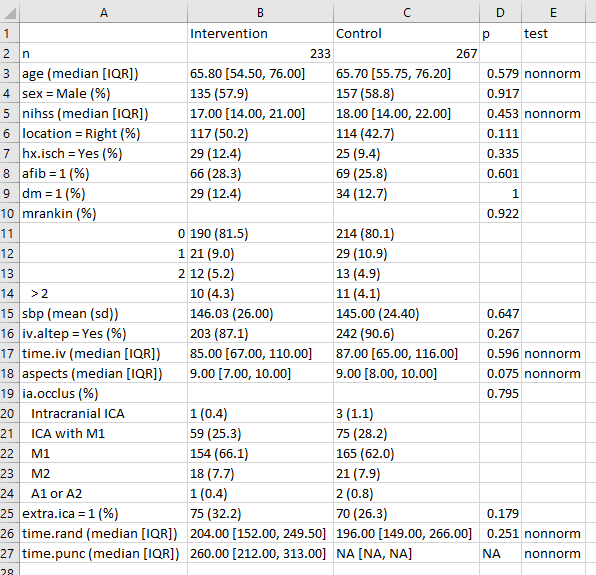
\includegraphics[width=0.9\linewidth]{images/fs-table1inExcel}

And from here, I can either drop it directly into Word, or present it as
is, or start tweaking it to meet formatting needs.

\subsection{Approach B: Produce the Table so you can cut and paste
it}\label{approach-b-produce-the-table-so-you-can-cut-and-paste-it}

\begin{Shaded}
\begin{Highlighting}[]
\KeywordTok{print}\NormalTok{(att2, }
      \DataTypeTok{nonnormal =} \KeywordTok{c}\NormalTok{(}\StringTok{"age"}\NormalTok{, }\StringTok{"nihss"}\NormalTok{, }\StringTok{"time.iv"}\NormalTok{, }\StringTok{"aspects"}\NormalTok{, }\StringTok{"time.rand"}\NormalTok{),}
      \DataTypeTok{exact =} \KeywordTok{c}\NormalTok{(}\StringTok{"location"}\NormalTok{, }\StringTok{"mrankin"}\NormalTok{),}
      \DataTypeTok{quote =} \OtherTok{TRUE}\NormalTok{, }\DataTypeTok{noSpaces =} \OtherTok{TRUE}\NormalTok{)}
\end{Highlighting}
\end{Shaded}

This will look like a mess by itself, but if you:

\begin{enumerate}
\def\labelenumi{\arabic{enumi}.}
\tightlist
\item
  copy and paste that mess into Excel
\item
  select Text to Columns from the Data menu
\item
  select Delimited, then Space and select Treat consecutive delimiters
  as one
\end{enumerate}

you should get something usable again.

Or, in Word,

\begin{enumerate}
\def\labelenumi{\arabic{enumi}.}
\tightlist
\item
  insert the text
\item
  select the text with your mouse
\item
  select Insert \ldots{} Table \ldots{} Convert Text to Table
\item
  place a quotation mark in the ``Other'' area under Separate text at
  \ldots{}
\end{enumerate}

After dropping blank columns, the result looks pretty good.

\section{A Controlled Biological Experiment - The Blood-Brain
Barrier}\label{a-controlled-biological-experiment---the-blood-brain-barrier}

My source for the data and the following explanatory paragraph is page
307 from \citet{RamseySchafer2002}. The original data come from
\citet{Barnett1995}.

\begin{quote}
The human brain (and that of rats, coincidentally) is protected from the
bacteria and toxins that course through the bloodstream by something
called the blood-brain barrier. After a method of disrupting the barrier
was developed, researchers tested this new mechanism, as follows. A
series of 34 rats were inoculated with human lung cancer cells to induce
brain tumors. After 9-11 days they were infused with either the barrier
disruption (BD) solution or, as a control, a normal saline (NS)
solution. Fifteen minutes later, the rats received a standard dose of a
particular therapeutic antibody (L6-F(ab')2. The key measure of the
effectiveness of transmission across the brain-blood barrier is the
ratio of the antibody concentration in the brain tumor to the antibody
concentration in normal tissue outside the brain. The rats were then
sacrificed, and the amounts of antibody in the brain tumor and in normal
tissue from the liver were measured. The study's primary objective is to
determine whether the antibody concentration in the tumor increased when
the blood-barrier disruption infusion was given, and if so, by how much?
\end{quote}

\section{\texorpdfstring{The \texttt{bloodbrain.csv}
file}{The bloodbrain.csv file}}\label{the-bloodbrain.csv-file}

Consider the data, available on the Data and Code page of
\href{https://github.com/THOMASELOVE/432-2018}{our course website} in
the \texttt{bloodbrain.csv} file, which includes the following
variables:

\begin{longtable}[]{@{}rl@{}}
\toprule
\begin{minipage}[b]{0.12\columnwidth}\raggedleft\strut
Variable\strut
\end{minipage} & \begin{minipage}[b]{0.59\columnwidth}\raggedright\strut
Description\strut
\end{minipage}\tabularnewline
\midrule
\endhead
\begin{minipage}[t]{0.12\columnwidth}\raggedleft\strut
\texttt{case}\strut
\end{minipage} & \begin{minipage}[t]{0.59\columnwidth}\raggedright\strut
identification number for the rat (1 - 34)\strut
\end{minipage}\tabularnewline
\begin{minipage}[t]{0.12\columnwidth}\raggedleft\strut
\texttt{brain}\strut
\end{minipage} & \begin{minipage}[t]{0.59\columnwidth}\raggedright\strut
an outcome: Brain tumor antibody count (per gram)\strut
\end{minipage}\tabularnewline
\begin{minipage}[t]{0.12\columnwidth}\raggedleft\strut
\texttt{liver}\strut
\end{minipage} & \begin{minipage}[t]{0.59\columnwidth}\raggedright\strut
an outcome: Liver antibody count (per gram)\strut
\end{minipage}\tabularnewline
\begin{minipage}[t]{0.12\columnwidth}\raggedleft\strut
\texttt{tlratio}\strut
\end{minipage} & \begin{minipage}[t]{0.59\columnwidth}\raggedright\strut
an outcome: tumor / liver concentration ratio\strut
\end{minipage}\tabularnewline
\begin{minipage}[t]{0.12\columnwidth}\raggedleft\strut
\texttt{solution}\strut
\end{minipage} & \begin{minipage}[t]{0.59\columnwidth}\raggedright\strut
the treatment: BD (barrier disruption) or NS (normal saline)\strut
\end{minipage}\tabularnewline
\begin{minipage}[t]{0.12\columnwidth}\raggedleft\strut
\texttt{sactime}\strut
\end{minipage} & \begin{minipage}[t]{0.59\columnwidth}\raggedright\strut
a design variable: Sacrifice time (hours; either 0.5, 3, 24 or 72)\strut
\end{minipage}\tabularnewline
\begin{minipage}[t]{0.12\columnwidth}\raggedleft\strut
\texttt{postin}\strut
\end{minipage} & \begin{minipage}[t]{0.59\columnwidth}\raggedright\strut
covariate: Days post-inoculation of lung cancer cells (9, 10 or
11)\strut
\end{minipage}\tabularnewline
\begin{minipage}[t]{0.12\columnwidth}\raggedleft\strut
\texttt{sex}\strut
\end{minipage} & \begin{minipage}[t]{0.59\columnwidth}\raggedright\strut
covariate: M or F\strut
\end{minipage}\tabularnewline
\begin{minipage}[t]{0.12\columnwidth}\raggedleft\strut
\texttt{wt.init}\strut
\end{minipage} & \begin{minipage}[t]{0.59\columnwidth}\raggedright\strut
covariate: Initial weight (grams)\strut
\end{minipage}\tabularnewline
\begin{minipage}[t]{0.12\columnwidth}\raggedleft\strut
\texttt{wt.loss}\strut
\end{minipage} & \begin{minipage}[t]{0.59\columnwidth}\raggedright\strut
covariate: Weight loss (grams)\strut
\end{minipage}\tabularnewline
\begin{minipage}[t]{0.12\columnwidth}\raggedleft\strut
\texttt{wt.tumor}\strut
\end{minipage} & \begin{minipage}[t]{0.59\columnwidth}\raggedright\strut
covariate: Tumor weight (10\textsuperscript{-4} grams)\strut
\end{minipage}\tabularnewline
\bottomrule
\end{longtable}

And here's what the data look like in R.

\begin{Shaded}
\begin{Highlighting}[]
\NormalTok{bloodbrain}
\end{Highlighting}
\end{Shaded}

\begin{verbatim}
# A tibble: 34 x 11
    case  brain   liver tlratio solution sactime postin sex   wt.init
   <int>  <int>   <int>   <dbl> <fct>      <dbl>  <int> <fct>   <int>
 1     1  41081 1456164  0.0282 BD         0.500     10 F         239
 2     2  44286 1602171  0.0276 BD         0.500     10 F         225
 3     3 102926 1601936  0.0642 BD         0.500     10 F         224
 4     4  25927 1776411  0.0146 BD         0.500     10 F         184
 5     5  42643 1351184  0.0316 BD         0.500     10 F         250
 6     6  31342 1790863  0.0175 NS         0.500     10 F         196
 7     7  22815 1633386  0.0140 NS         0.500     10 F         200
 8     8  16629 1618757  0.0103 NS         0.500     10 F         273
 9     9  22315 1567602  0.0142 NS         0.500     10 F         216
10    10  77961 1060057  0.0735 BD         3.00      10 F         267
# ... with 24 more rows, and 2 more variables: wt.loss <dbl>, wt.tumor
#   <int>
\end{verbatim}

\section{\texorpdfstring{A Table 1 for
\texttt{bloodbrain}}{A Table 1 for bloodbrain}}\label{a-table-1-for-bloodbrain}

\citet{Barnett1995} did not provide a Table 1 for these data, so let's
build one to compare the two \texttt{solutions} (\texttt{BD} vs.
\texttt{NS}) on the covariates and outcomes, plus the natural logarithm
of the tumor/liver concentration ratio (\texttt{tlratio}). We'll opt to
treat the sacrifice time (\texttt{sactime}) and the days
post-inoculation of lung cancer cells (\texttt{postin}) as categorical
rather than quantitative variables.

\begin{Shaded}
\begin{Highlighting}[]
\NormalTok{bloodbrain <-}\StringTok{ }\NormalTok{bloodbrain }\OperatorTok
\StringTok{    }\KeywordTok{mutate}\NormalTok{(}\DataTypeTok{logTL =} \KeywordTok{log}\NormalTok{(tlratio))}

\KeywordTok{dput}\NormalTok{(}\KeywordTok{names}\NormalTok{(bloodbrain))}
\end{Highlighting}
\end{Shaded}

\begin{verbatim}
c("case", "brain", "liver", "tlratio", "solution", "sactime", 
"postin", "sex", "wt.init", "wt.loss", "wt.tumor", "logTL")
\end{verbatim}

OK - there's the list of variables we'll need. I'll put the outcomes at
the bottom of the table.

\begin{Shaded}
\begin{Highlighting}[]
\NormalTok{bb.vars <-}\StringTok{ }\KeywordTok{c}\NormalTok{(}\StringTok{"sactime"}\NormalTok{, }\StringTok{"postin"}\NormalTok{, }\StringTok{"sex"}\NormalTok{, }\StringTok{"wt.init"}\NormalTok{, }\StringTok{"wt.loss"}\NormalTok{, }
             \StringTok{"wt.tumor"}\NormalTok{, }\StringTok{"brain"}\NormalTok{, }\StringTok{"liver"}\NormalTok{, }\StringTok{"tlratio"}\NormalTok{, }\StringTok{"logTL"}\NormalTok{)}

\NormalTok{bb.factors <-}\StringTok{ }\KeywordTok{c}\NormalTok{(}\StringTok{"sactime"}\NormalTok{, }\StringTok{"sex"}\NormalTok{, }\StringTok{"postin"}\NormalTok{)}

\NormalTok{bb.att1 <-}\StringTok{ }\KeywordTok{CreateTableOne}\NormalTok{(}\DataTypeTok{data =}\NormalTok{ bloodbrain,}
                          \DataTypeTok{vars =}\NormalTok{ bb.vars,}
                          \DataTypeTok{factorVars =}\NormalTok{ bb.factors,}
                          \DataTypeTok{strata =} \KeywordTok{c}\NormalTok{(}\StringTok{"solution"}\NormalTok{))}
\KeywordTok{summary}\NormalTok{(bb.att1)}
\end{Highlighting}
\end{Shaded}

\begin{verbatim}

     ### Summary of continuous variables ###

solution: BD
          n miss p.miss   mean    sd median    p25   p75    min   max
wt.init  17    0      0    243 3e+01  2e+02  2e+02 3e+02  2e+02 3e+02
wt.loss  17    0      0      3 5e+00  4e+00  1e+00 6e+00 -5e+00 1e+01
wt.tumor 17    0      0    157 8e+01  2e+02  1e+02 2e+02  2e+01 4e+02
brain    17    0      0  56043 3e+04  5e+04  4e+04 8e+04  6e+03 1e+05
liver    17    0      0 672577 7e+05  6e+05  2e+04 1e+06  2e+03 2e+06
tlratio  17    0      0      2 3e+00  1e-01  6e-02 3e+00  1e-02 9e+00
logTL    17    0      0     -1 2e+00 -2e+00 -3e+00 1e+00 -4e+00 2e+00
          skew kurt
wt.init  -0.39  0.7
wt.loss  -0.10  0.2
wt.tumor  0.53  1.0
brain     0.29 -0.6
liver     0.35 -1.7
tlratio   1.58  1.7
logTL     0.08 -1.7
-------------------------------------------------------- 
solution: NS
          n miss p.miss   mean    sd median    p25    p75    min   max
wt.init  17    0      0    240 3e+01  2e+02  2e+02  3e+02  2e+02 3e+02
wt.loss  17    0      0      4 4e+00  3e+00  2e+00  7e+00 -4e+00 1e+01
wt.tumor 17    0      0    209 1e+02  2e+02  2e+02  3e+02  3e+01 5e+02
brain    17    0      0  23887 1e+04  2e+04  1e+04  3e+04  1e+03 5e+04
liver    17    0      0 664975 7e+05  7e+05  2e+04  1e+06  9e+02 2e+06
tlratio  17    0      0      1 2e+00  5e-02  3e-02  9e-01  1e-02 7e+00
logTL    17    0      0     -2 2e+00 -3e+00 -3e+00 -7e-02 -5e+00 2e+00
          skew  kurt
wt.init   0.33 -0.48
wt.loss  -0.09  0.08
wt.tumor  0.63  0.77
brain     0.30 -0.35
liver     0.40 -1.56
tlratio   2.27  4.84
logTL     0.27 -1.61

p-values
             pNormal  pNonNormal
wt.init  0.807308940 0.641940278
wt.loss  0.683756156 0.876749808
wt.tumor 0.151510151 0.190482094
brain    0.001027678 0.002579901
liver    0.974853609 0.904045603
tlratio  0.320501715 0.221425879
logTL    0.351633525 0.221425879

Standardize mean differences
             1 vs 2
wt.init  0.08435244
wt.loss  0.14099823
wt.tumor 0.50397184
brain    1.23884159
liver    0.01089667
tlratio  0.34611465
logTL    0.32420504

=======================================================================================

     ### Summary of categorical variables ### 

solution: BD
     var  n miss p.miss level freq percent cum.percent
 sactime 17    0    0.0   0.5    5    29.4        29.4
                            3    4    23.5        52.9
                           24    4    23.5        76.5
                           72    4    23.5       100.0
                                                      
  postin 17    0    0.0     9    1     5.9         5.9
                           10   14    82.4        88.2
                           11    2    11.8       100.0
                                                      
     sex 17    0    0.0     F   13    76.5        76.5
                            M    4    23.5       100.0
                                                      
-------------------------------------------------------- 
solution: NS
     var  n miss p.miss level freq percent cum.percent
 sactime 17    0    0.0   0.5    4    23.5        23.5
                            3    5    29.4        52.9
                           24    4    23.5        76.5
                           72    4    23.5       100.0
                                                      
  postin 17    0    0.0     9    2    11.8        11.8
                           10   13    76.5        88.2
                           11    2    11.8       100.0
                                                      
     sex 17    0    0.0     F   13    76.5        76.5
                            M    4    23.5       100.0
                                                      

p-values
          pApprox pExact
sactime 0.9739246      1
postin  0.8309504      1
sex     1.0000000      1

Standardize mean differences
           1 vs 2
sactime 0.1622214
postin  0.2098877
sex     0.0000000
\end{verbatim}

Note that, in this particular case, the decisions we make about
normality vs.~non-normality (for quantitative variables) and the
decisions we make about approximate vs.~exact testing (for categorical
variables) won't actually change the implications of the \emph{p}
values. Each approach gives similar results for each variable. Of
course, that's not always true.

\subsection{\texorpdfstring{Generate final Table 1 for
\texttt{bloodbrain}}{Generate final Table 1 for bloodbrain}}\label{generate-final-table-1-for-bloodbrain}

I'll choose to treat \texttt{tlratio} and its logarithm as non-Normal,
but otherwise, use t tests, but admittedly, that's an arbitrary
decision, really.

\begin{Shaded}
\begin{Highlighting}[]
\KeywordTok{print}\NormalTok{(bb.att1, }\DataTypeTok{nonnormal =} \KeywordTok{c}\NormalTok{(}\StringTok{"tlratio"}\NormalTok{, }\StringTok{"logTL"}\NormalTok{))}
\end{Highlighting}
\end{Shaded}

\begin{verbatim}
                        Stratified by solution
                         BD                      NS                      
  n                             17                      17               
  sactime (%)                                                            
     0.5                         5 (29.4)                4 (23.5)        
     3                           4 (23.5)                5 (29.4)        
     24                          4 (23.5)                4 (23.5)        
     72                          4 (23.5)                4 (23.5)        
  postin (%)                                                             
     9                           1 ( 5.9)                2 (11.8)        
     10                         14 (82.4)               13 (76.5)        
     11                          2 (11.8)                2 (11.8)        
  sex = M (%)                    4 (23.5)                4 (23.5)        
  wt.init (mean (sd))       242.82 (27.23)          240.47 (28.54)       
  wt.loss (mean (sd))         3.34 (4.68)             3.94 (3.88)        
  wt.tumor (mean (sd))      157.29 (84.00)          208.53 (116.68)      
  brain (mean (sd))       56043.41 (33675.40)     23887.18 (14610.53)    
  liver (mean (sd))      672577.35 (694479.58)   664975.47 (700773.13)   
  tlratio (median [IQR])      0.12 [0.06, 2.84]       0.05 [0.03, 0.94]  
  logTL (median [IQR])       -2.10 [-2.74, 1.04]     -2.95 [-3.41, -0.07]
                        Stratified by solution
                         p      test   
  n                                    
  sactime (%)             0.974        
     0.5                               
     3                                 
     24                                
     72                                
  postin (%)              0.831        
     9                                 
     10                                
     11                                
  sex = M (%)             1.000        
  wt.init (mean (sd))     0.807        
  wt.loss (mean (sd))     0.684        
  wt.tumor (mean (sd))    0.152        
  brain (mean (sd))       0.001        
  liver (mean (sd))       0.975        
  tlratio (median [IQR])  0.221 nonnorm
  logTL (median [IQR])    0.221 nonnorm
\end{verbatim}

Or, we can get an Excel-readable version placed in a \texttt{data}
subfolder, using

\begin{Shaded}
\begin{Highlighting}[]
\NormalTok{bb.t1 <-}\StringTok{ }\KeywordTok{print}\NormalTok{(bb.att1, }\DataTypeTok{nonnormal =} \KeywordTok{c}\NormalTok{(}\StringTok{"tlratio"}\NormalTok{, }\StringTok{"logTL"}\NormalTok{), }\DataTypeTok{quote =} \OtherTok{FALSE}\NormalTok{,}
               \DataTypeTok{noSpaces =} \OtherTok{TRUE}\NormalTok{, }\DataTypeTok{printToggle =} \OtherTok{FALSE}\NormalTok{)}

\KeywordTok{write.csv}\NormalTok{(bb.t1, }\DataTypeTok{file =} \StringTok{"data/bb-table1.csv"}\NormalTok{)}
\end{Highlighting}
\end{Shaded}

which, when dropped into Excel, will look like this:

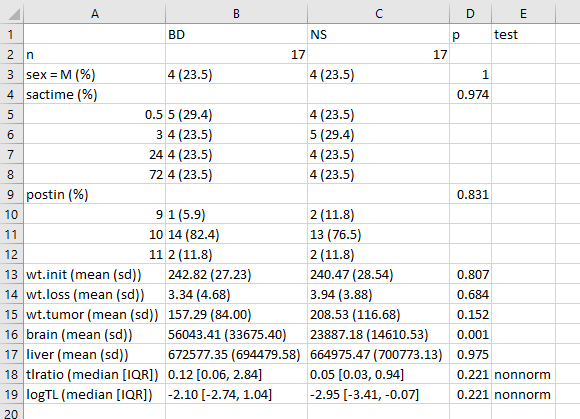
\includegraphics[width=0.9\linewidth]{images/bb-table1inExcel}

One thing I would definitely clean up here, in practice, is to change
the presentation of the \emph{p} value for \texttt{sex} from 1 to
\textgreater{} 0.99, or just omit it altogether. I'd also drop the
\texttt{computer-ese} where possible, add units for the measures, round
\textbf{a lot}, identify the outcomes carefully, and use notes to
indicate deviations from the main approach.

\subsection{A More Finished Version (after Cleanup in
Word)}\label{a-more-finished-version-after-cleanup-in-word}

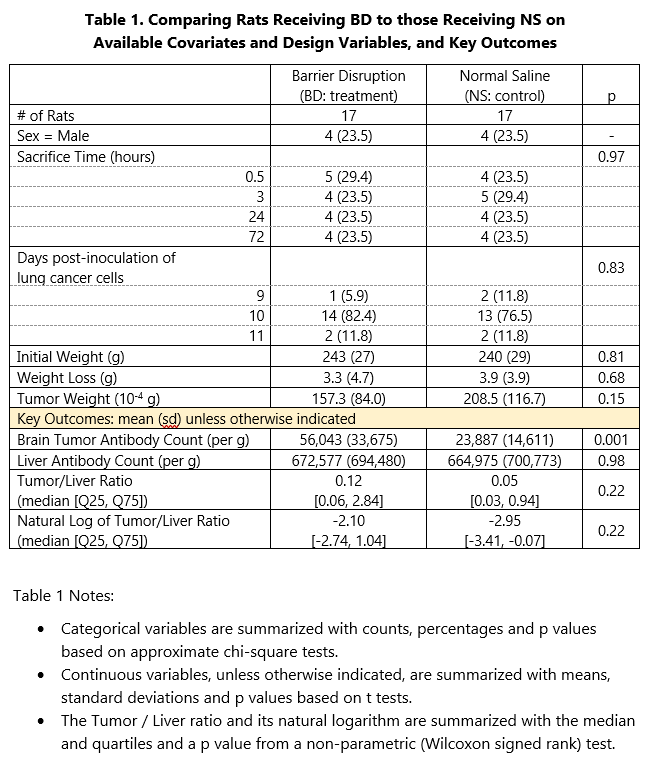
\includegraphics[width=0.95\linewidth]{images/bb-table1inWord}

\chapter{Linear Regression on a small SMART data
set}\label{linear-regression-on-a-small-smart-data-set}

\section{BRFSS and SMART}\label{brfss-and-smart}

The Centers for Disease Control analyzes Behavioral Risk Factor
Surveillance System (BRFSS) survey data for specific metropolitan and
micropolitan statistical areas (MMSAs) in a program called the
\href{https://www.cdc.gov/brfss/smart/Smart_data.htm}{Selected
Metropolitan/Micropolitan Area Risk Trends of BRFSS} (SMART BRFSS.)

In this work, we will focus on
\href{https://www.cdc.gov/brfss/smart/smart_2016.html}{data from the
2016 SMART}, and in particular on data from the Cleveland-Elyria, OH,
Metropolitan Statistical Area. The purpose of this survey is to provide
localized health information that can help public health practitioners
identify local emerging health problems, plan and evaluate local
responses, and efficiently allocate resources to specific needs.

\subsection{Key resources}\label{key-resources}

\begin{itemize}
\tightlist
\item
  the full data are available in the form of the 2016 SMART BRFSS MMSA
  Data, found in a zipped
  \href{https://www.cdc.gov/brfss/smart/2016/MMSA2016_XPT.zip}{SAS
  Transport Format} file. The data were released in August 2017.
\item
  the
  \href{https://www.cdc.gov/brfss/smart/2016/mmsa_varlayout_16.pdf}{MMSA
  Variable Layout PDF} which simply lists the variables included in the
  data file
\item
  the
  \href{https://www.cdc.gov/brfss/annual_data/2016/pdf/2016_calculated_variables_version4.pdf}{Calculated
  Variables PDF} which describes the risk factors by data variable names
  - there is also an
  \href{https://www.cdc.gov/brfss/annual_data/2016/Summary_Matrix_16.html}{online
  summary matrix of these calculated variables}, as well.
\item
  the lengthy
  \href{https://www.cdc.gov/brfss/questionnaires/pdf-ques/2016_BRFSS_Questionnaire_FINAL.pdf}{2016
  Survey Questions PDF} which lists all questions asked as part of the
  BRFSS in 2016
\item
  the enormous
  \href{https://www.cdc.gov/brfss/annual_data/2016/pdf/codebook16_llcp.pdf}{Codebook
  for the 2016 BRFSS Survey PDF} which identifies the variables by name
  for us.
\end{itemize}

Later this term, we'll use all of those resources to help construct a
more complete data set than we'll study today. I'll also demonstrate how
I built the \texttt{smartcle1} data set that we'll use in this Chapter.

\section{\texorpdfstring{The \texttt{smartcle1} data:
Cookbook}{The smartcle1 data: Cookbook}}\label{the-smartcle1-data-cookbook}

The \texttt{smartcle1.csv} data file available on the Data and Code page
of \href{https://github.com/THOMASELOVE/432-2018}{our website} describes
information on 11 variables for 1036 respondents to the BRFSS 2016, who
live in the Cleveland-Elyria, OH, Metropolitan Statistical Area. The
variables in the \texttt{smartcle1.csv} file are listed below, along
with (in some cases) the BRFSS items that generate these responses.

\begin{longtable}[]{@{}rl@{}}
\toprule
\begin{minipage}[b]{0.14\columnwidth}\raggedleft\strut
Variable\strut
\end{minipage} & \begin{minipage}[b]{0.74\columnwidth}\raggedright\strut
Description\strut
\end{minipage}\tabularnewline
\midrule
\endhead
\begin{minipage}[t]{0.14\columnwidth}\raggedleft\strut
\texttt{SEQNO}\strut
\end{minipage} & \begin{minipage}[t]{0.74\columnwidth}\raggedright\strut
respondent identification number (all begin with 2016)\strut
\end{minipage}\tabularnewline
\begin{minipage}[t]{0.14\columnwidth}\raggedleft\strut
\texttt{physhealth}\strut
\end{minipage} & \begin{minipage}[t]{0.74\columnwidth}\raggedright\strut
Now thinking about your physical health, which includes physical illness
and injury, for how many days during the past 30 days was your physical
health not good?\strut
\end{minipage}\tabularnewline
\begin{minipage}[t]{0.14\columnwidth}\raggedleft\strut
\texttt{menthealth}\strut
\end{minipage} & \begin{minipage}[t]{0.74\columnwidth}\raggedright\strut
Now thinking about your mental health, which includes stress,
depression, and problems with emotions, for how many days during the
past 30 days was your mental health not good?\strut
\end{minipage}\tabularnewline
\begin{minipage}[t]{0.14\columnwidth}\raggedleft\strut
\texttt{poorhealth}\strut
\end{minipage} & \begin{minipage}[t]{0.74\columnwidth}\raggedright\strut
During the past 30 days, for about how many days did poor physical or
mental health keep you from doing your usual activities, such as
self-care, work, or recreation?\strut
\end{minipage}\tabularnewline
\begin{minipage}[t]{0.14\columnwidth}\raggedleft\strut
\texttt{genhealth}\strut
\end{minipage} & \begin{minipage}[t]{0.74\columnwidth}\raggedright\strut
Would you say that in general, your health is \ldots{} (five categories:
Excellent, Very Good, Good, Fair or Poor)\strut
\end{minipage}\tabularnewline
\begin{minipage}[t]{0.14\columnwidth}\raggedleft\strut
\texttt{bmi}\strut
\end{minipage} & \begin{minipage}[t]{0.74\columnwidth}\raggedright\strut
Body mass index, in kg/m\textsuperscript{2}\strut
\end{minipage}\tabularnewline
\begin{minipage}[t]{0.14\columnwidth}\raggedleft\strut
\texttt{female}\strut
\end{minipage} & \begin{minipage}[t]{0.74\columnwidth}\raggedright\strut
Sex, 1 = female, 0 = male\strut
\end{minipage}\tabularnewline
\begin{minipage}[t]{0.14\columnwidth}\raggedleft\strut
\texttt{internet30}\strut
\end{minipage} & \begin{minipage}[t]{0.74\columnwidth}\raggedright\strut
Have you used the internet in the past 30 days? (1 = yes, 0 = no)\strut
\end{minipage}\tabularnewline
\begin{minipage}[t]{0.14\columnwidth}\raggedleft\strut
\texttt{exerany}\strut
\end{minipage} & \begin{minipage}[t]{0.74\columnwidth}\raggedright\strut
During the past month, other than your regular job, did you participate
in any physical activities or exercises such as running, calisthenics,
golf, gardening, or walking for exercise? (1 = yes, 0 = no)\strut
\end{minipage}\tabularnewline
\begin{minipage}[t]{0.14\columnwidth}\raggedleft\strut
\texttt{sleephrs}\strut
\end{minipage} & \begin{minipage}[t]{0.74\columnwidth}\raggedright\strut
On average, how many hours of sleep do you get in a 24-hour
period?\strut
\end{minipage}\tabularnewline
\begin{minipage}[t]{0.14\columnwidth}\raggedleft\strut
\texttt{alcdays}\strut
\end{minipage} & \begin{minipage}[t]{0.74\columnwidth}\raggedright\strut
How many days during the past 30 days did you have at least one drink of
any alcoholic beverage such as beer, wine, a malt beverage or
liquor?\strut
\end{minipage}\tabularnewline
\bottomrule
\end{longtable}

\begin{Shaded}
\begin{Highlighting}[]
\KeywordTok{str}\NormalTok{(smartcle1)}
\end{Highlighting}
\end{Shaded}

\begin{verbatim}
Classes 'tbl_df', 'tbl' and 'data.frame':   1036 obs. of  11 variables:
 $ SEQNO     : num  2.02e+09 2.02e+09 2.02e+09 2.02e+09 2.02e+09 ...
 $ physhealth: int  0 0 1 0 5 4 2 2 0 0 ...
 $ menthealth: int  0 0 5 0 0 18 0 3 0 0 ...
 $ poorhealth: int  NA NA 0 NA 0 6 0 0 NA NA ...
 $ genhealth : Factor w/ 5 levels "1_Excellent",..: 2 1 2 3 1 2 3 3 2 3 ...
 $ bmi       : num  26.7 23.7 26.9 21.7 24.1 ...
 $ female    : int  1 0 0 1 0 0 1 1 0 0 ...
 $ internet30: int  1 1 1 1 1 1 1 1 1 1 ...
 $ exerany   : int  1 1 0 1 1 1 1 1 1 0 ...
 $ sleephrs  : int  6 6 8 9 7 5 9 7 7 7 ...
 $ alcdays   : int  1 4 4 3 2 28 4 2 4 25 ...
\end{verbatim}

\section{\texorpdfstring{\texttt{smartcle2}: Omitting Missing
Observations: Complete-Case
Analyses}{smartcle2: Omitting Missing Observations: Complete-Case Analyses}}\label{smartcle2-omitting-missing-observations-complete-case-analyses}

For the purpose of fitting our first few models, we will eliminate the
missingness problem, and look only at the \emph{complete cases} in our
\texttt{smartcle1} data. We will discuss methods for imputing missing
data later in these Notes.

To inspect the missingness in our data, we might consider using the
\texttt{skim} function from the \texttt{skimr} package. We'll exclude
the respondent identifier code (\texttt{SEQNO}) from this summary as
uninteresting.

\begin{Shaded}
\begin{Highlighting}[]
\KeywordTok{skim_with}\NormalTok{(}\DataTypeTok{numeric =} \KeywordTok{list}\NormalTok{(}\DataTypeTok{hist =} \OtherTok{NULL}\NormalTok{), }\DataTypeTok{integer =} \KeywordTok{list}\NormalTok{(}\DataTypeTok{hist =} \OtherTok{NULL}\NormalTok{))}
\NormalTok{## above line eliminates the sparkline histograms}
\NormalTok{## it can be commented out when working in the console,}
\NormalTok{## but I need it to produce the Notes without errors right now}

\NormalTok{smartcle1 }\OperatorTok\StringTok{ }
\StringTok{    }\KeywordTok{skim}\NormalTok{(}\OperatorTok{-}\NormalTok{SEQNO)}
\end{Highlighting}
\end{Shaded}

\begin{verbatim}
Skim summary statistics
 n obs: 1036 
 n variables: 11 

Variable type: factor 
  variable missing complete    n n_unique
 genhealth       3     1033 1036        5
                             top_counts ordered
 2_V: 350, 3_G: 344, 1_E: 173, 4_F: 122   FALSE

Variable type: integer 
   variable missing complete    n mean   sd p0 p25 median p75 p100
    alcdays      46      990 1036 4.65 8.05  0   0      1   4   30
    exerany       3     1033 1036 0.76 0.43  0   1      1   1    1
     female       0     1036 1036 0.6  0.49  0   0      1   1    1
 internet30       6     1030 1036 0.81 0.39  0   1      1   1    1
 menthealth      11     1025 1036 2.72 6.82  0   0      0   2   30
 physhealth      17     1019 1036 3.97 8.67  0   0      0   2   30
 poorhealth     543      493 1036 4.07 8.09  0   0      0   3   30
   sleephrs       8     1028 1036 7.02 1.53  1   6      7   8   20

Variable type: numeric 
 variable missing complete    n  mean   sd    p0  p25 median   p75  p100
      bmi      84      952 1036 27.89 6.47 12.71 23.7  26.68 30.53 66.06
\end{verbatim}

Now, we'll create a new tibble called \texttt{smartcle2} which contains
every variable except \texttt{poorhealth}, and which includes all
respondents with complete data on the variables (other than
\texttt{poorhealth}). We'll store those observations with complete data
in the \texttt{smartcle2} tibble.

\begin{Shaded}
\begin{Highlighting}[]
\NormalTok{smartcle2 <-}\StringTok{ }\NormalTok{smartcle1 }\OperatorTok\StringTok{ }
\StringTok{    }\KeywordTok{select}\NormalTok{(}\OperatorTok{-}\NormalTok{poorhealth) }\OperatorTok
\StringTok{    }\KeywordTok{filter}\NormalTok{(}\KeywordTok{complete.cases}\NormalTok{(.))}

\NormalTok{smartcle2}
\end{Highlighting}
\end{Shaded}

\begin{verbatim}
# A tibble: 896 x 10
     SEQNO physhealth menthealth genhealth   bmi female internet30 exerany
     <dbl>      <int>      <int> <fct>     <dbl>  <int>      <int>   <int>
 1  2.02e9          0          0 2_VeryGo~  26.7      1          1       1
 2  2.02e9          0          0 1_Excell~  23.7      0          1       1
 3  2.02e9          1          5 2_VeryGo~  26.9      0          1       0
 4  2.02e9          0          0 3_Good     21.7      1          1       1
 5  2.02e9          5          0 1_Excell~  24.1      0          1       1
 6  2.02e9          4         18 2_VeryGo~  27.6      0          1       1
 7  2.02e9          2          0 3_Good     25.7      1          1       1
 8  2.02e9          2          3 3_Good     28.5      1          1       1
 9  2.02e9          0          0 2_VeryGo~  28.6      0          1       1
10  2.02e9          0          0 3_Good     23.1      0          1       0
# ... with 886 more rows, and 2 more variables: sleephrs <int>, alcdays
#   <int>
\end{verbatim}

Note that there are only 896 respondents with \textbf{complete} data on
the 10 variables (excluding \texttt{poorhealth}) in the
\texttt{smartcle2} tibble, as compared to our original
\texttt{smartcle1} data which described 1036 respondents and 11
variables, but with lots of missing data.

\section{\texorpdfstring{Summarizing the \texttt{smartcle2} data
numerically}{Summarizing the smartcle2 data numerically}}\label{summarizing-the-smartcle2-data-numerically}

\subsection{\texorpdfstring{The New Toy: The \texttt{skim}
function}{The New Toy: The skim function}}\label{the-new-toy-the-skim-function}

\begin{Shaded}
\begin{Highlighting}[]
\KeywordTok{skim}\NormalTok{(smartcle2, }\OperatorTok{-}\NormalTok{SEQNO)}
\end{Highlighting}
\end{Shaded}

\begin{verbatim}
Skim summary statistics
 n obs: 896 
 n variables: 10 

Variable type: factor 
  variable missing complete   n n_unique
 genhealth       0      896 896        5
                             top_counts ordered
 2_V: 306, 3_G: 295, 1_E: 155, 4_F: 102   FALSE

Variable type: integer 
   variable missing complete   n mean   sd p0 p25 median p75 p100
    alcdays       0      896 896 4.83 8.14  0   0      1   5   30
    exerany       0      896 896 0.77 0.42  0   1      1   1    1
     female       0      896 896 0.58 0.49  0   0      1   1    1
 internet30       0      896 896 0.81 0.39  0   1      1   1    1
 menthealth       0      896 896 2.69 6.72  0   0      0   2   30
 physhealth       0      896 896 3.99 8.64  0   0      0   2   30
   sleephrs       0      896 896 7.02 1.48  1   6      7   8   20

Variable type: numeric 
 variable missing complete   n  mean   sd    p0  p25 median   p75  p100
      bmi       0      896 896 27.87 6.33 12.71 23.7   26.8 30.53 66.06
\end{verbatim}

\subsection{\texorpdfstring{The usual \texttt{summary} for a data
frame}{The usual summary for a data frame}}\label{the-usual-summary-for-a-data-frame}

Of course, we can use the usual \texttt{summary} to get some basic
information about the data.

\begin{Shaded}
\begin{Highlighting}[]
\KeywordTok{summary}\NormalTok{(smartcle2)}
\end{Highlighting}
\end{Shaded}

\begin{verbatim}
     SEQNO             physhealth      menthealth           genhealth  
 Min.   :2.016e+09   Min.   : 0.00   Min.   : 0.000   1_Excellent:155  
 1st Qu.:2.016e+09   1st Qu.: 0.00   1st Qu.: 0.000   2_VeryGood :306  
 Median :2.016e+09   Median : 0.00   Median : 0.000   3_Good     :295  
 Mean   :2.016e+09   Mean   : 3.99   Mean   : 2.693   4_Fair     :102  
 3rd Qu.:2.016e+09   3rd Qu.: 2.00   3rd Qu.: 2.000   5_Poor     : 38  
 Max.   :2.016e+09   Max.   :30.00   Max.   :30.000                    
      bmi            female         internet30        exerany      
 Min.   :12.71   Min.   :0.0000   Min.   :0.0000   Min.   :0.0000  
 1st Qu.:23.70   1st Qu.:0.0000   1st Qu.:1.0000   1st Qu.:1.0000  
 Median :26.80   Median :1.0000   Median :1.0000   Median :1.0000  
 Mean   :27.87   Mean   :0.5848   Mean   :0.8147   Mean   :0.7667  
 3rd Qu.:30.53   3rd Qu.:1.0000   3rd Qu.:1.0000   3rd Qu.:1.0000  
 Max.   :66.06   Max.   :1.0000   Max.   :1.0000   Max.   :1.0000  
    sleephrs         alcdays      
 Min.   : 1.000   Min.   : 0.000  
 1st Qu.: 6.000   1st Qu.: 0.000  
 Median : 7.000   Median : 1.000  
 Mean   : 7.022   Mean   : 4.834  
 3rd Qu.: 8.000   3rd Qu.: 5.000  
 Max.   :20.000   Max.   :30.000  
\end{verbatim}

\subsection{\texorpdfstring{The \texttt{describe} function in
\texttt{Hmisc}}{The describe function in Hmisc}}\label{the-describe-function-in-hmisc}

Or we can use the \texttt{describe} function from the \texttt{Hmisc}
package.

\begin{Shaded}
\begin{Highlighting}[]
\NormalTok{Hmisc}\OperatorTok{::}\KeywordTok{describe}\NormalTok{(}\KeywordTok{select}\NormalTok{(smartcle2, bmi, genhealth, female))}
\end{Highlighting}
\end{Shaded}

\begin{verbatim}
select(smartcle2, bmi, genhealth, female) 

 3  Variables      896  Observations
---------------------------------------------------------------------------
bmi 
       n  missing distinct     Info     Mean      Gmd      .05      .10 
     896        0      467        1    27.87    6.572    20.06    21.23 
     .25      .50      .75      .90      .95 
   23.70    26.80    30.53    35.36    39.30 

lowest : 12.71 13.34 14.72 16.22 17.30, highest: 56.89 57.04 60.95 61.84 66.06
---------------------------------------------------------------------------
genhealth 
       n  missing distinct 
     896        0        5 
                                                                      
Value      1_Excellent  2_VeryGood      3_Good      4_Fair      5_Poor
Frequency          155         306         295         102          38
Proportion       0.173       0.342       0.329       0.114       0.042
---------------------------------------------------------------------------
female 
       n  missing distinct     Info      Sum     Mean      Gmd 
     896        0        2    0.728      524   0.5848   0.4862 

---------------------------------------------------------------------------
\end{verbatim}

\section{Counting as exploratory data
analysis}\label{counting-as-exploratory-data-analysis}

Counting things can be amazingly useful.

\subsection{How many respondents had exercised in the past 30 days? Did
this vary by
sex?}\label{how-many-respondents-had-exercised-in-the-past-30-days-did-this-vary-by-sex}

\begin{Shaded}
\begin{Highlighting}[]
\NormalTok{smartcle2 }\OperatorTok\StringTok{ }\KeywordTok{count}\NormalTok{(female, exerany) }\OperatorTok\StringTok{ }\KeywordTok{mutate}\NormalTok{(}\DataTypeTok{percent =} \DecValTok{100}\OperatorTok{*}\NormalTok{n }\OperatorTok{/}\StringTok{ }\KeywordTok{sum}\NormalTok{(n))}
\end{Highlighting}
\end{Shaded}

\begin{verbatim}
# A tibble: 4 x 4
  female exerany     n percent
   <int>   <int> <int>   <dbl>
1      0       0    64    7.14
2      0       1   308   34.4 
3      1       0   145   16.2 
4      1       1   379   42.3 
\end{verbatim}

so we know now that 42.3\% of the subjects in our data were women who
exercised. Suppose that instead we want to find the percentage of
exercisers within each sex\ldots{}

\begin{Shaded}
\begin{Highlighting}[]
\NormalTok{smartcle2 }\OperatorTok
\StringTok{    }\KeywordTok{count}\NormalTok{(female, exerany) }\OperatorTok
\StringTok{    }\KeywordTok{group_by}\NormalTok{(female) }\OperatorTok
\StringTok{    }\KeywordTok{mutate}\NormalTok{(}\DataTypeTok{prob =} \DecValTok{100}\OperatorTok{*}\NormalTok{n }\OperatorTok{/}\StringTok{ }\KeywordTok{sum}\NormalTok{(n)) }
\end{Highlighting}
\end{Shaded}

\begin{verbatim}
# A tibble: 4 x 4
# Groups: female [2]
  female exerany     n  prob
   <int>   <int> <int> <dbl>
1      0       0    64  17.2
2      0       1   308  82.8
3      1       0   145  27.7
4      1       1   379  72.3
\end{verbatim}

and now we know that 82.8\% of the males exercised at least once in the
last 30 days, as compared to 72.3\% of the females.

\subsection{\texorpdfstring{What's the distribution of
\texttt{sleephrs}?}{What's the distribution of sleephrs?}}\label{whats-the-distribution-of-sleephrs}

We can count quantitative variables with discrete sets of possible
values, like \texttt{sleephrs}, which is captured as an integer (that
must fall between 0 and 24.)

\begin{Shaded}
\begin{Highlighting}[]
\NormalTok{smartcle2 }\OperatorTok\StringTok{ }\KeywordTok{count}\NormalTok{(sleephrs)}
\end{Highlighting}
\end{Shaded}

\begin{verbatim}
# A tibble: 14 x 2
   sleephrs     n
      <int> <int>
 1        1     5
 2        2     1
 3        3     6
 4        4    20
 5        5    63
 6        6   192
 7        7   276
 8        8   266
 9        9    38
10       10    22
11       11     2
12       12     2
13       16     2
14       20     1
\end{verbatim}

Of course, a natural summary of a quantitative variable like this would
be graphical.

\begin{Shaded}
\begin{Highlighting}[]
\KeywordTok{ggplot}\NormalTok{(smartcle2, }\KeywordTok{aes}\NormalTok{(sleephrs)) }\OperatorTok{+}
\StringTok{    }\KeywordTok{geom_histogram}\NormalTok{(}\DataTypeTok{binwidth =} \DecValTok{1}\NormalTok{, }\DataTypeTok{fill =} \StringTok{"dodgerblue"}\NormalTok{, }\DataTypeTok{col =} \StringTok{"darkred"}\NormalTok{)}
\end{Highlighting}
\end{Shaded}

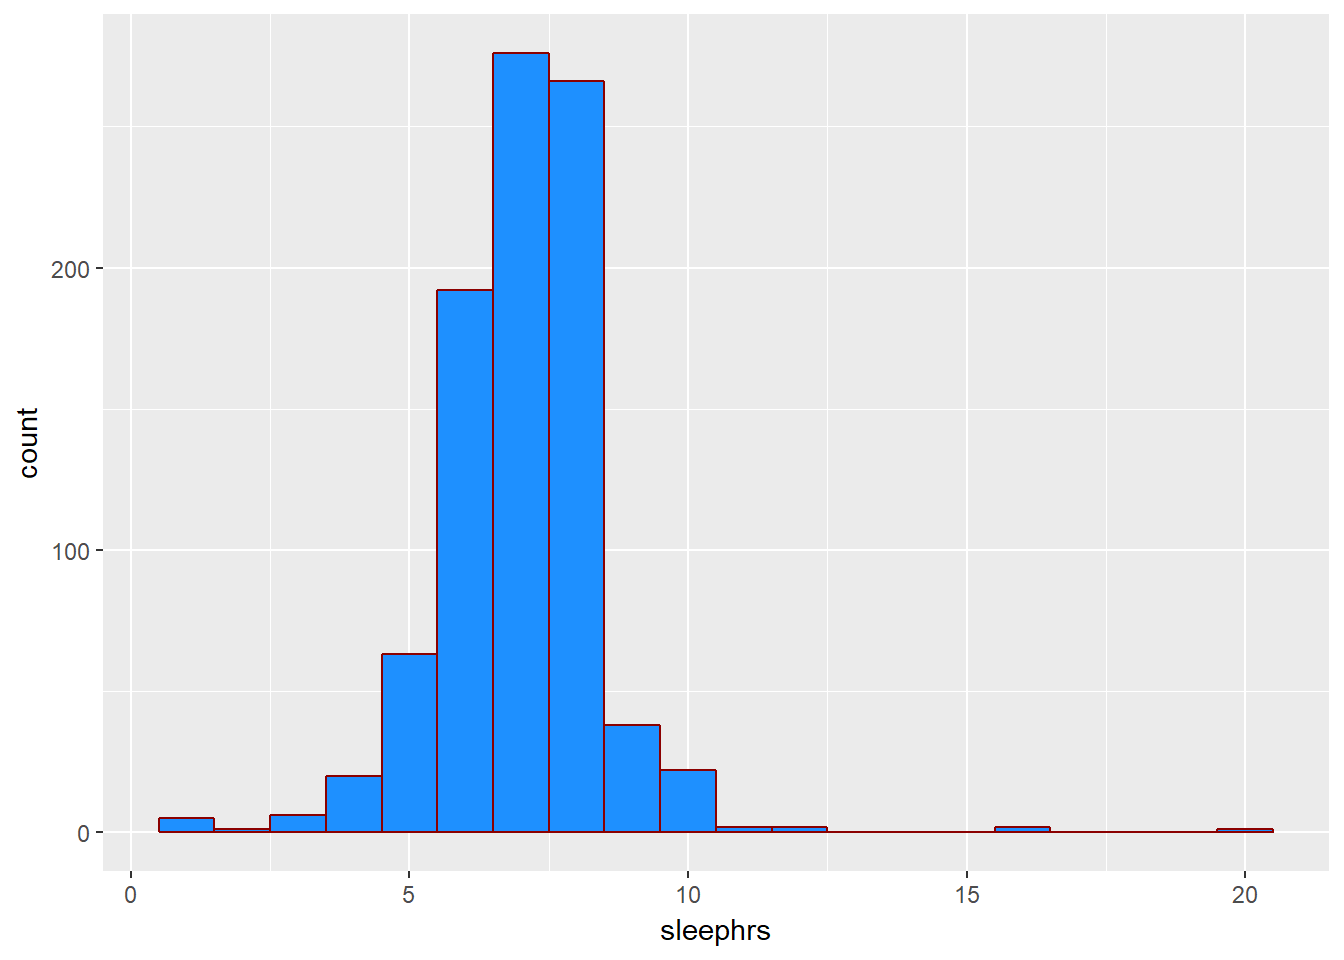
\includegraphics{bookdown-demo_files/figure-latex/c2_histogram_sleephrs_smartcle2-1.pdf}

\subsection{\texorpdfstring{What's the distribution of
\texttt{BMI}?}{What's the distribution of BMI?}}\label{whats-the-distribution-of-bmi}

\begin{Shaded}
\begin{Highlighting}[]
\KeywordTok{ggplot}\NormalTok{(smartcle2, }\KeywordTok{aes}\NormalTok{(bmi)) }\OperatorTok{+}
\StringTok{    }\KeywordTok{geom_histogram}\NormalTok{(}\DataTypeTok{bins =} \DecValTok{30}\NormalTok{, }\DataTypeTok{col =} \StringTok{"white"}\NormalTok{)}
\end{Highlighting}
\end{Shaded}

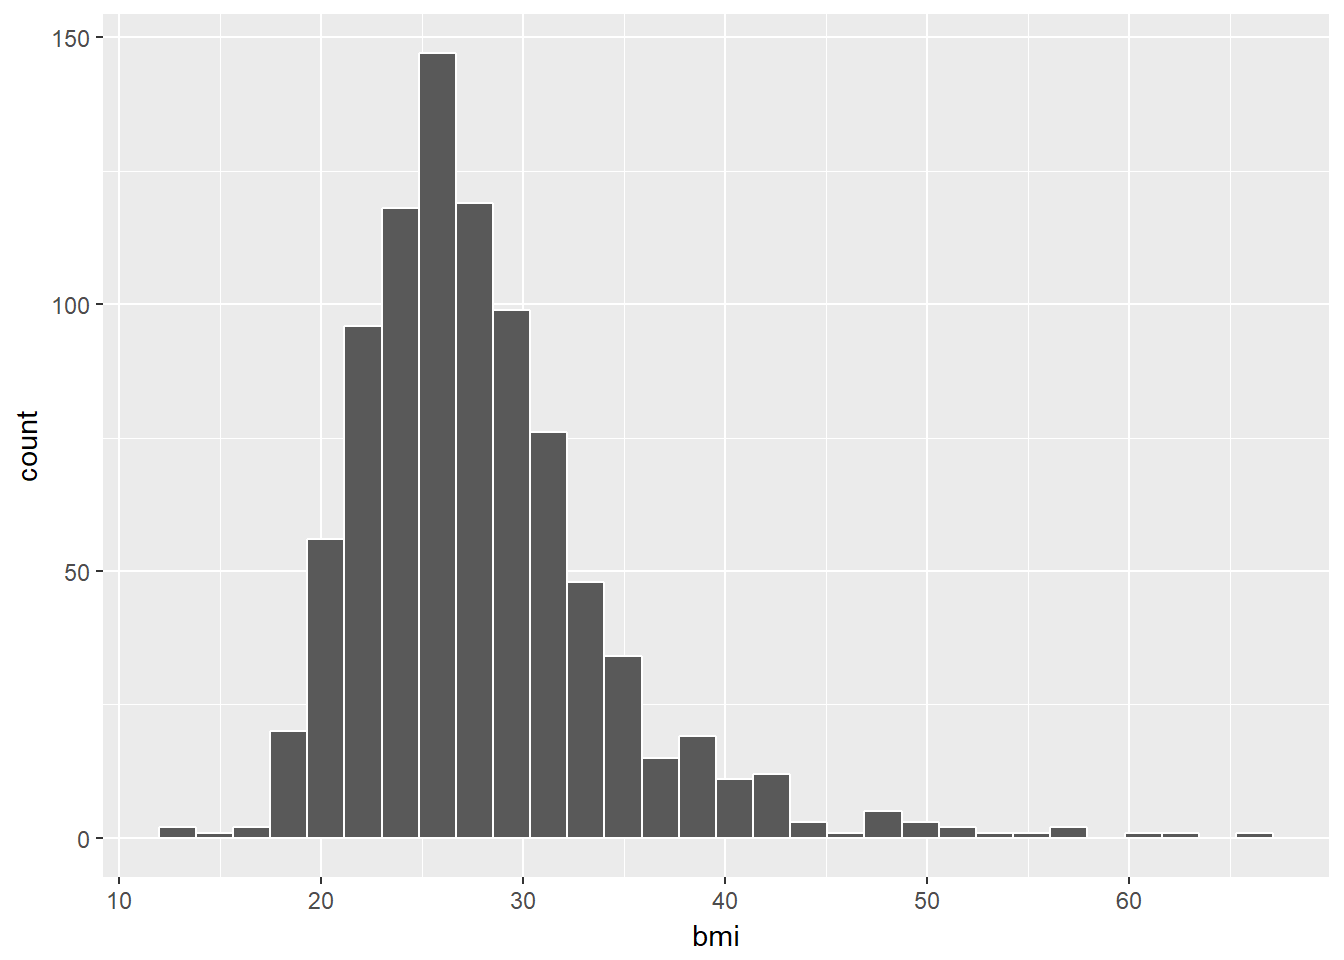
\includegraphics{bookdown-demo_files/figure-latex/c2_histogram_bmi_smartcle2-1.pdf}

\subsection{How many of the respondents have a BMI below
30?}\label{how-many-of-the-respondents-have-a-bmi-below-30}

\begin{Shaded}
\begin{Highlighting}[]
\NormalTok{smartcle2 }\OperatorTok\StringTok{ }\KeywordTok{count}\NormalTok{(bmi }\OperatorTok{<}\StringTok{ }\DecValTok{30}\NormalTok{) }\OperatorTok\StringTok{ }\KeywordTok{mutate}\NormalTok{(}\DataTypeTok{proportion =}\NormalTok{ n }\OperatorTok{/}\StringTok{ }\KeywordTok{sum}\NormalTok{(n))}
\end{Highlighting}
\end{Shaded}

\begin{verbatim}
# A tibble: 2 x 3
  `bmi < 30`     n proportion
  <lgl>      <int>      <dbl>
1 F            253      0.282
2 T            643      0.718
\end{verbatim}

\subsection{How many of the respondents who have a BMI \textless{} 30
exercised?}\label{how-many-of-the-respondents-who-have-a-bmi-30-exercised}

\begin{Shaded}
\begin{Highlighting}[]
\NormalTok{smartcle2 }\OperatorTok\StringTok{ }\KeywordTok{count}\NormalTok{(exerany, bmi }\OperatorTok{<}\StringTok{ }\DecValTok{30}\NormalTok{) }\OperatorTok
\StringTok{    }\KeywordTok{group_by}\NormalTok{(exerany) }\OperatorTok
\StringTok{    }\KeywordTok{mutate}\NormalTok{(}\DataTypeTok{percent =} \DecValTok{100}\OperatorTok{*}\NormalTok{n}\OperatorTok{/}\KeywordTok{sum}\NormalTok{(n))}
\end{Highlighting}
\end{Shaded}

\begin{verbatim}
# A tibble: 4 x 4
# Groups: exerany [2]
  exerany `bmi < 30`     n percent
    <int> <lgl>      <int>   <dbl>
1       0 F             88    42.1
2       0 T            121    57.9
3       1 F            165    24.0
4       1 T            522    76.0
\end{verbatim}

\subsection{Is obesity associated with sex, in these
data?}\label{is-obesity-associated-with-sex-in-these-data}

\begin{Shaded}
\begin{Highlighting}[]
\NormalTok{smartcle2 }\OperatorTok\StringTok{ }\KeywordTok{count}\NormalTok{(female, bmi }\OperatorTok{<}\StringTok{ }\DecValTok{30}\NormalTok{) }\OperatorTok
\StringTok{    }\KeywordTok{group_by}\NormalTok{(female) }\OperatorTok
\StringTok{    }\KeywordTok{mutate}\NormalTok{(}\DataTypeTok{percent =} \DecValTok{100}\OperatorTok{*}\NormalTok{n}\OperatorTok{/}\KeywordTok{sum}\NormalTok{(n))}
\end{Highlighting}
\end{Shaded}

\begin{verbatim}
# A tibble: 4 x 4
# Groups: female [2]
  female `bmi < 30`     n percent
   <int> <lgl>      <int>   <dbl>
1      0 F            105    28.2
2      0 T            267    71.8
3      1 F            148    28.2
4      1 T            376    71.8
\end{verbatim}

\subsection{\texorpdfstring{Comparing \texttt{sleephrs} summaries by
obesity
status}{Comparing sleephrs summaries by obesity status}}\label{comparing-sleephrs-summaries-by-obesity-status}

Can we compare the \texttt{sleephrs} means, medians and
75\textsuperscript{th} percentiles for respondents whose BMI is below 30
to the respondents whose BMI is not?

\begin{Shaded}
\begin{Highlighting}[]
\NormalTok{smartcle2 }\OperatorTok
\StringTok{    }\KeywordTok{group_by}\NormalTok{(bmi }\OperatorTok{<}\StringTok{ }\DecValTok{30}\NormalTok{) }\OperatorTok
\StringTok{    }\KeywordTok{summarize}\NormalTok{(}\KeywordTok{mean}\NormalTok{(sleephrs), }\KeywordTok{median}\NormalTok{(sleephrs), }
              \DataTypeTok{q75 =} \KeywordTok{quantile}\NormalTok{(sleephrs, }\FloatTok{0.75}\NormalTok{))}
\end{Highlighting}
\end{Shaded}

\begin{verbatim}
# A tibble: 2 x 4
  `bmi < 30` `mean(sleephrs)` `median(sleephrs)`   q75
  <lgl>                 <dbl>              <int> <dbl>
1 F                      6.93                  7  8.00
2 T                      7.06                  7  8.00
\end{verbatim}

\subsection{\texorpdfstring{The \texttt{skim} function within a
pipe}{The skim function within a pipe}}\label{the-skim-function-within-a-pipe}

The \textbf{skim} function works within pipes and with the other
\texttt{tidyverse} functions.

\begin{Shaded}
\begin{Highlighting}[]
\NormalTok{smartcle2 }\OperatorTok
\StringTok{    }\KeywordTok{group_by}\NormalTok{(exerany) }\OperatorTok
\StringTok{    }\KeywordTok{skim}\NormalTok{(bmi, sleephrs)}
\end{Highlighting}
\end{Shaded}

\begin{verbatim}
Skim summary statistics
 n obs: 896 
 n variables: 10 
 group variables: exerany 

Variable type: integer 
 exerany variable missing complete   n mean   sd p0 p25 median p75 p100
       0 sleephrs       0      209 209 7    1.85  1   6      7   8   20
       1 sleephrs       0      687 687 7.03 1.34  1   6      7   8   16

Variable type: numeric 
 exerany variable missing complete   n  mean   sd    p0   p25 median   p75
       0      bmi       0      209 209 29.57 7.46 18    24.11  28.49 33.13
       1      bmi       0      687 687 27.35 5.84 12.71 23.7   26.52 29.81
  p100
 66.06
 60.95
\end{verbatim}

\section{\texorpdfstring{First Modeling Attempt: Can \texttt{bmi}
predict
\texttt{physhealth}?}{First Modeling Attempt: Can bmi predict physhealth?}}\label{first-modeling-attempt-can-bmi-predict-physhealth}

We'll start with an effort to predict \texttt{physhealth} using
\texttt{bmi}. A natural graph would be a scatterplot.

\begin{Shaded}
\begin{Highlighting}[]
\KeywordTok{ggplot}\NormalTok{(}\DataTypeTok{data =}\NormalTok{ smartcle2, }\KeywordTok{aes}\NormalTok{(}\DataTypeTok{x =}\NormalTok{ bmi, }\DataTypeTok{y =}\NormalTok{ physhealth)) }\OperatorTok{+}
\StringTok{    }\KeywordTok{geom_point}\NormalTok{()}
\end{Highlighting}
\end{Shaded}

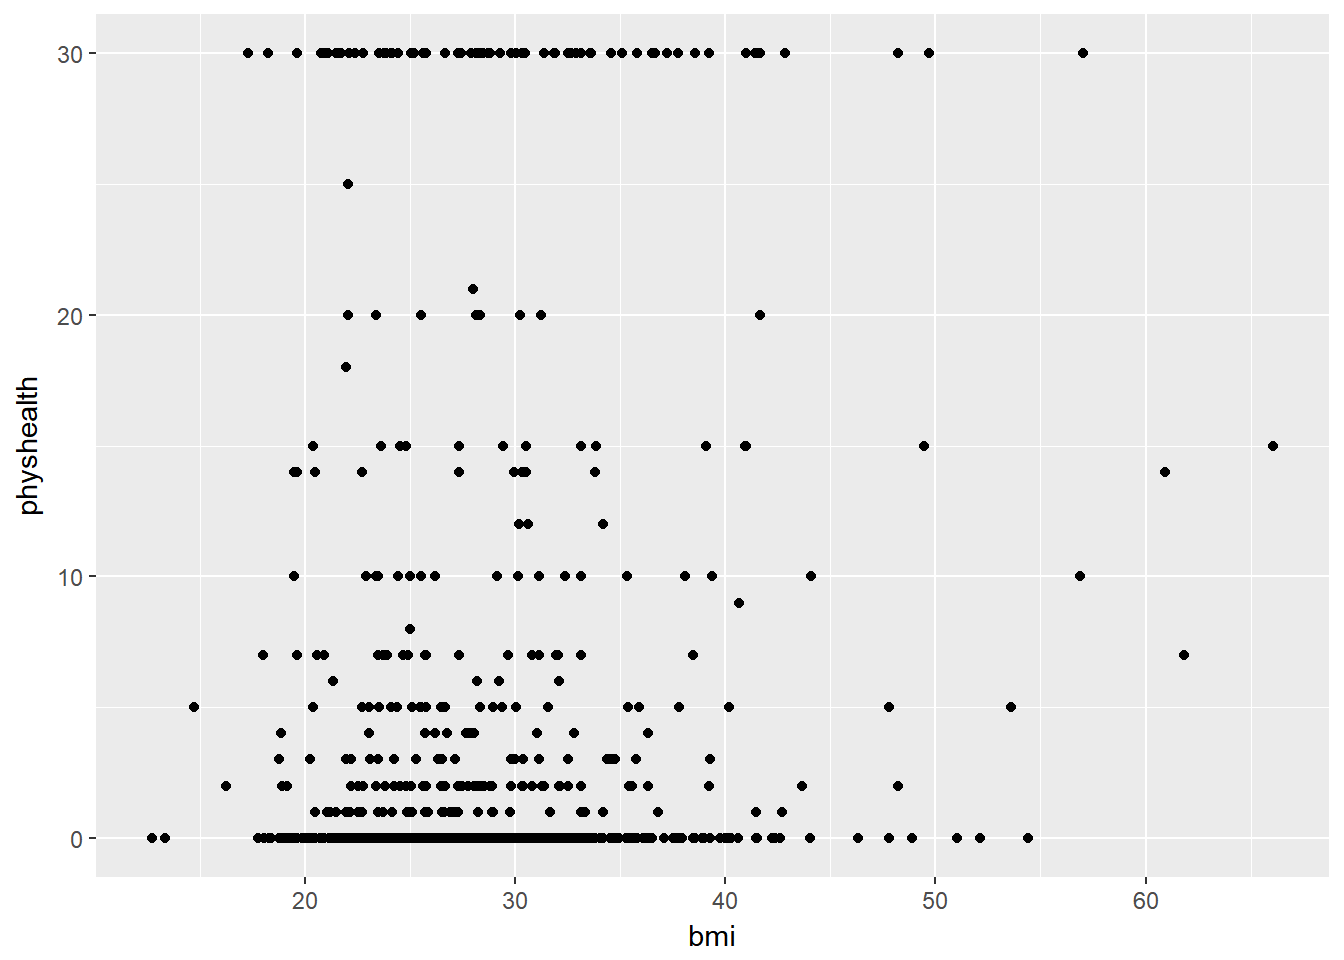
\includegraphics{bookdown-demo_files/figure-latex/scatter_physhealth_bmi_1-1.pdf}

A good question to ask ourselves here might be: ``In what BMI range can
we make a reasonable prediction of \texttt{physhealth}?''

Now, we might take the plot above and add a simple linear model \ldots{}

\begin{Shaded}
\begin{Highlighting}[]
\KeywordTok{ggplot}\NormalTok{(}\DataTypeTok{data =}\NormalTok{ smartcle2, }\KeywordTok{aes}\NormalTok{(}\DataTypeTok{x =}\NormalTok{ bmi, }\DataTypeTok{y =}\NormalTok{ physhealth)) }\OperatorTok{+}
\StringTok{    }\KeywordTok{geom_point}\NormalTok{() }\OperatorTok{+}
\StringTok{    }\KeywordTok{geom_smooth}\NormalTok{(}\DataTypeTok{method =} \StringTok{"lm"}\NormalTok{, }\DataTypeTok{se =} \OtherTok{FALSE}\NormalTok{)}
\end{Highlighting}
\end{Shaded}

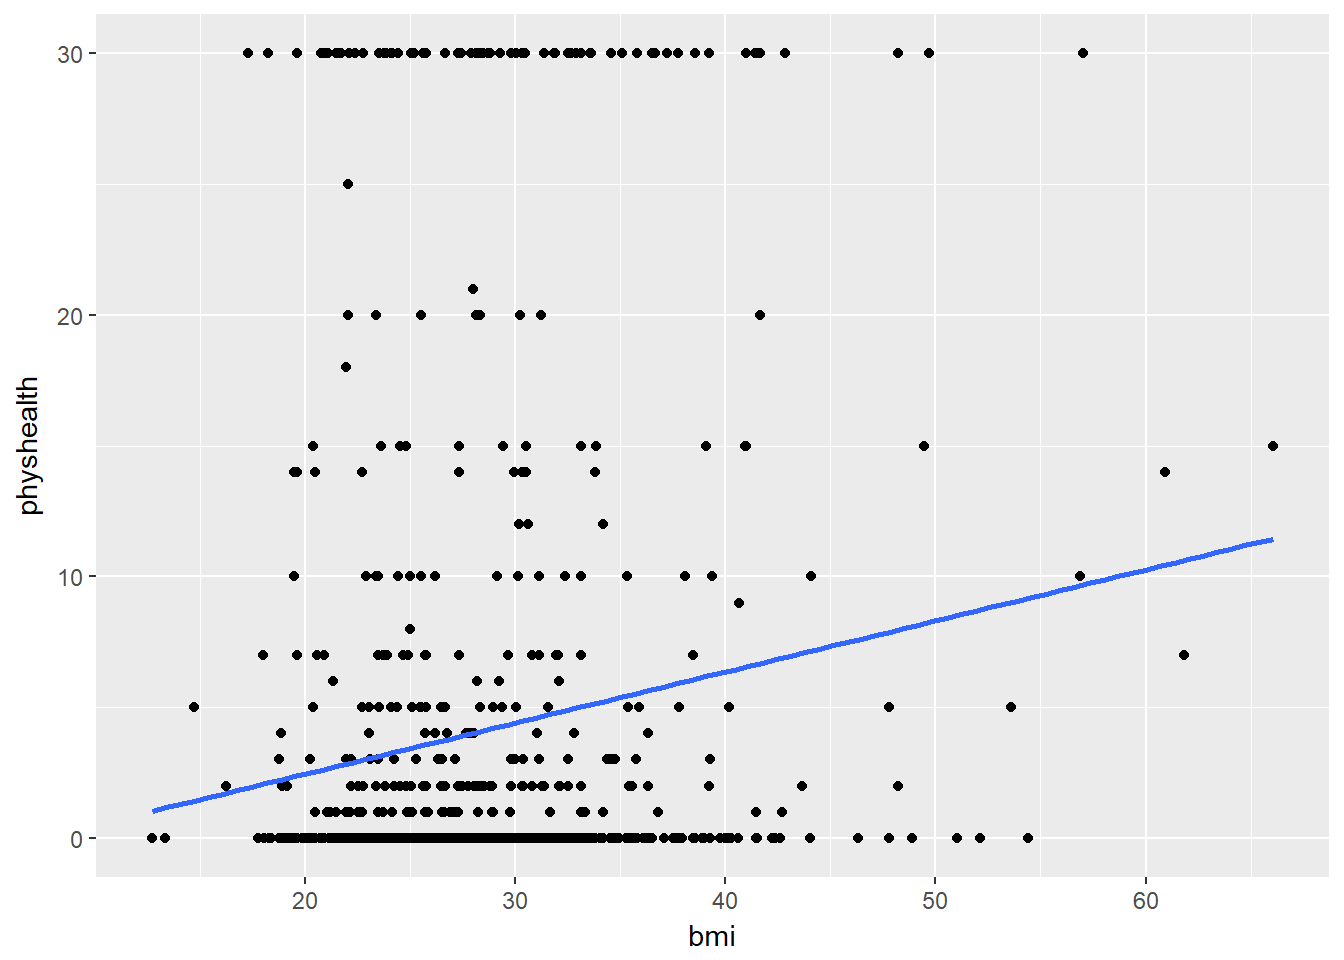
\includegraphics{bookdown-demo_files/figure-latex/c2_scatter_physhealth_bmi_2-1.pdf}

which shows the same least squares regression model that we can fit with
the \texttt{lm} command.

\subsection{Fitting a Simple Regression
Model}\label{fitting-a-simple-regression-model}

\begin{Shaded}
\begin{Highlighting}[]
\NormalTok{model_A <-}\StringTok{ }\KeywordTok{lm}\NormalTok{(physhealth }\OperatorTok{~}\StringTok{ }\NormalTok{bmi, }\DataTypeTok{data =}\NormalTok{ smartcle2)}

\NormalTok{model_A}
\end{Highlighting}
\end{Shaded}

\begin{verbatim}

Call:
lm(formula = physhealth ~ bmi, data = smartcle2)

Coefficients:
(Intercept)          bmi  
    -1.4514       0.1953  
\end{verbatim}

\begin{Shaded}
\begin{Highlighting}[]
\KeywordTok{summary}\NormalTok{(model_A)}
\end{Highlighting}
\end{Shaded}

\begin{verbatim}

Call:
lm(formula = physhealth ~ bmi, data = smartcle2)

Residuals:
   Min     1Q Median     3Q    Max 
-9.171 -4.057 -3.193 -1.576 28.073 

Coefficients:
            Estimate Std. Error t value Pr(>|t|)    
(Intercept) -1.45143    1.29185  -1.124    0.262    
bmi          0.19527    0.04521   4.319 1.74e-05 ***
---
Signif. codes:  0 '***' 0.001 '**' 0.01 '*' 0.05 '.' 0.1 ' ' 1

Residual standard error: 8.556 on 894 degrees of freedom
Multiple R-squared:  0.02044,   Adjusted R-squared:  0.01934 
F-statistic: 18.65 on 1 and 894 DF,  p-value: 1.742e-05
\end{verbatim}

\begin{Shaded}
\begin{Highlighting}[]
\KeywordTok{confint}\NormalTok{(model_A, }\DataTypeTok{level =} \FloatTok{0.95}\NormalTok{)}
\end{Highlighting}
\end{Shaded}

\begin{verbatim}
                 2.5 %    97.5 %
(Intercept) -3.9868457 1.0839862
bmi          0.1065409 0.2840068
\end{verbatim}

The model coefficients can be obtained by printing the model object, and
the \texttt{summary} function provides several useful descriptions of
the model's residuals, its statistical significance, and quality of fit.

\subsection{Model Summary for a Simple (One-Predictor)
Regression}\label{model-summary-for-a-simple-one-predictor-regression}

The fitted model predicts \texttt{physhealth} with the equation -1.45 +
0.195*\texttt{bmi}, as we can read off from the model coefficients.

Each of the 896 respondents included in the \texttt{smartcle2} data
makes a contribution to this model.

\subsubsection{Residuals}\label{residuals}

Suppose Harry is one of the people in that group, and Harry's data is
\texttt{bmi} = 20, and \texttt{physhealth} = 3.

\begin{itemize}
\tightlist
\item
  Harry's \emph{observed} value of \texttt{physhealth} is just the value
  we have in the data for them, in this case, observed
  \texttt{physhealth} = 3 for Harry.
\item
  Harry's \emph{fitted} or \emph{predicted} \texttt{physhealth} value is
  the result of calculating -1.45 + 0.195*\texttt{bmi} for Harry. So, if
  Harry's BMI was 20, then Harry's predicted \texttt{physhealth} value
  is -1.45 + (0.195)(20) = 2.45.
\item
  The \emph{residual} for Harry is then his \emph{observed} outcome
  minus his \emph{fitted} outcome, so Harry has a residual of 3 - 2.45 =
  0.55.
\item
  Graphically, a residual represents vertical distance between the
  observed point and the fitted regression line.
\item
  Points above the regression line will have positive residuals, and
  points below the regression line will have negative residuals. Points
  on the line have zero residuals.
\end{itemize}

The residuals are summarized at the top of the \texttt{summary} output
for linear model.

\begin{itemize}
\tightlist
\item
  The mean residual will always be zero in an ordinary least squares
  model, but a five number summary of the residuals is provided by the
  summary, as is an estimated standard deviation of the residuals
  (called here the Residual standard error.)
\item
  In the \texttt{smartcle2} data, the minimum residual was -9.17, so for
  one subject, the observed value was 9.17 days smaller than the
  predicted value. This means that the prediction was 9.17 days too
  large for that subject.
\item
  Similarly, the maximum residual was 28.07 days, so for one subject the
  prediction was 28.07 days too small. Not a strong performance.
\item
  In a least squares model, the residuals are assumed to follow a Normal
  distribution, with mean zero, and standard deviation (for the
  \texttt{smartcle2} data) of about 8.6 days. Thus, by the definition of
  a Normal distribution, we'd expect
\item
  about 68\% of the residuals to be between -8.6 and +8.6 days,
\item
  about 95\% of the residuals to be between -17.2 and +17.2 days,
\item
  about all (99.7\%) of the residuals to be between -25.8 and +25.8
  days.
\end{itemize}

\subsubsection{Coefficients section}\label{coefficients-section}

The \texttt{summary} for a linear model shows Estimates, Standard
Errors, t values and \emph{p} values for each coefficient fit.

\begin{itemize}
\tightlist
\item
  The Estimates are the point estimates of the intercept and slope of
  \texttt{bmi} in our model.
\item
  In this case, our estimated slope is 0.195, which implies that if
  Harry's BMI is 20 and Sally's BMI is 21, we predict that Sally's
  \texttt{physhealth} will be 0.195 days larger than Harry's.
\item
  The Standard Errors are also provided for each estimate. We can create
  rough 95\% confidence intervals by adding and subtracting two standard
  errors from each coefficient, or we can get a slightly more accurate
  answer with the \texttt{confint} function.
\item
  Here, the 95\% confidence interval for the slope of \texttt{bmi} is
  estimated to be (0.11, 0.28). This is a good measure of the
  uncertainty in the slope that is captured by our model. We are 95\%
  confident in the process of building this interval, but this doesn't
  mean we're 95\% sure that the true slope is actually in that interval.
\end{itemize}

Also available are a \emph{t} value (just the Estimate divided by the
Standard Error) and the appropriate \emph{p} value for testing the null
hypothesis that the true value of the coefficient is 0 against a
two-tailed alternative.

\begin{itemize}
\tightlist
\item
  If a slope coefficient is statistically significantly different from
  0, this implies that 0 will not be part of the uncertainty interval
  obtained through \texttt{confint}.
\item
  If the slope was zero, it would suggest that \texttt{bmi} would add no
  predictive value to the model. But that's unlikely here.
\end{itemize}

If the \texttt{bmi} slope coefficient is associated with a small
\emph{p} value, as in the case of our \texttt{model\_A}, it suggests
that the model including \texttt{bmi} is statistically significantly
better at predicting \texttt{physhealth} than the model without
\texttt{bmi}.

\begin{itemize}
\tightlist
\item
  Without \texttt{bmi} our \texttt{model\_A} would become an
  \emph{intercept-only} model, in this case, which would predict the
  mean \texttt{physhealth} for everyone, regardless of any other
  information.
\end{itemize}

\subsubsection{Model Fit Summaries}\label{model-fit-summaries}

The \texttt{summary} of a linear model also displays:

\begin{itemize}
\tightlist
\item
  The residual standard error and associated degrees of freedom for the
  residuals.
\item
  For a simple (one-predictor) least regression like this, the residual
  degrees of freedom will be the sample size minus 2.
\item
  The multiple R-squared (or coefficient of determination)
\item
  This is interpreted as the proportion of variation in the outcome
  (\texttt{physhealth}) accounted for by the model, and will always fall
  between 0 and 1 as a result.
\item
  Our model\_A accounts for a mere 2\% of the variation in
  \texttt{physhealth}.
\item
  The Adjusted R-squared value ``adjusts'' for the size of our model in
  terms of the number of coefficients included in the model.
\item
  The adjusted R-squared will always be less than the Multiple
  R-squared.
\item
  We still hope to find models with relatively large adjusted
  R\textsuperscript{2} values.
\item
  In particular, we hope to find models where the adjusted
  R\textsuperscript{2} isn't substantially less than the Multiple
  R-squared.
\item
  The adjusted R-squared is usually a better estimate of likely
  performance of our model in new data than is the Multiple R-squared.
\item
  The adjusted R-squared result is no longer interpretable as a
  proportion of anything - in fact, it can fall below 0.
\item
  We can obtain the adjusted R\textsuperscript{2} from the raw
  R\textsuperscript{2}, the number of observations \emph{N} and the
  number of predictors \emph{p} included in the model, as follows:
\end{itemize}

\[
R^2_{adj} = 1 - \frac{(1 - R^2)(N - 1)}{N - p - 1},
\]

\begin{itemize}
\tightlist
\item
  The F statistic and \emph{p} value from a global ANOVA test of the
  model.

  \begin{itemize}
  \tightlist
  \item
    Obtaining a statistically significant result here is usually pretty
    straightforward, since the comparison is between our model, and a
    model which simply predicts the mean value of the outcome for
    everyone.
  \item
    In a simple (one-predictor) linear regression like this, the t
    statistic for the slope is just the square root of the F statistic,
    and the resulting \emph{p} values for the slope's t test and for the
    global F test will be identical.
  \end{itemize}
\item
  To see the complete ANOVA F test for this model, we can run
  \texttt{anova(model\_A)}.
\end{itemize}

\begin{Shaded}
\begin{Highlighting}[]
\KeywordTok{anova}\NormalTok{(model_A)}
\end{Highlighting}
\end{Shaded}

\begin{verbatim}
Analysis of Variance Table

Response: physhealth
           Df Sum Sq Mean Sq F value    Pr(>F)    
bmi         1   1366  1365.5  18.655 1.742e-05 ***
Residuals 894  65441    73.2                      
---
Signif. codes:  0 '***' 0.001 '**' 0.01 '*' 0.05 '.' 0.1 ' ' 1
\end{verbatim}

\subsection{\texorpdfstring{Using the \texttt{broom}
package}{Using the broom package}}\label{using-the-broom-package}

The \texttt{broom} package has three functions of particular use in a
linear regression model:

\subsubsection{\texorpdfstring{The \texttt{tidy}
function}{The tidy function}}\label{the-tidy-function}

\texttt{tidy} builds a data frame/tibble containing information about
the coefficients in the model, their standard errors, t statistics and
\emph{p} values.

\begin{Shaded}
\begin{Highlighting}[]
\KeywordTok{tidy}\NormalTok{(model_A)}
\end{Highlighting}
\end{Shaded}

\begin{verbatim}
         term   estimate  std.error statistic      p.value
1 (Intercept) -1.4514298 1.29185199 -1.123526 2.615156e-01
2         bmi  0.1952739 0.04521145  4.319125 1.741859e-05
\end{verbatim}

\subsubsection{\texorpdfstring{The \texttt{glance}
function}{The glance function}}\label{the-glance-function}

glance` builds a data frame/tibble containing summary statistics about
the model, including

\begin{itemize}
\tightlist
\item
  the (raw) multiple R\textsuperscript{2} and adjusted R\^{}2
\item
  \texttt{sigma} which is the residual standard error
\item
  the F \texttt{statistic}, \texttt{p.value} model \texttt{df} and
  \texttt{df.residual} associated with the global ANOVA test, plus
\item
  several statistics that will be useful in comparing models down the
  line:
\item
  the model's log likelihood function value, \texttt{logLik}
\item
  the model's Akaike's Information Criterion value, \texttt{AIC}
\item
  the model's Bayesian Information Criterion value, \texttt{BIC}
\item
  and the model's \texttt{deviance} statistic
\end{itemize}

\begin{Shaded}
\begin{Highlighting}[]
\KeywordTok{glance}\NormalTok{(model_A)}
\end{Highlighting}
\end{Shaded}

\begin{verbatim}
   r.squared adj.r.squared    sigma statistic      p.value df    logLik
1 0.02044019    0.01934449 8.555737  18.65484 1.741859e-05  2 -3193.723
       AIC     BIC deviance df.residual
1 6393.446 6407.84 65441.36         894
\end{verbatim}

\subsubsection{\texorpdfstring{The \texttt{augment}
function}{The augment function}}\label{the-augment-function}

\texttt{augment} builds a data frame/tibble which adds fitted values,
residuals and other diagnostic summaries that describe each observation
to the original data used to fit the model, and this includes

\begin{itemize}
\tightlist
\item
  \texttt{.fitted} and \texttt{.resid}, the fitted and residual values,
  in addition to
\item
  \texttt{.hat}, the leverage value for this observation
\item
  \texttt{.cooksd}, the Cook's distance measure of \emph{influence} for
  this observation
\item
  \texttt{.stdresid}, the standardized residual (think of this as a
  z-score - a measure of the residual divided by its associated standard
  deviation \texttt{.sigma})
\item
  and \texttt{se.fit} which will help us generate prediction intervals
  for the model downstream
\end{itemize}

Note that each of the new columns begins with \texttt{.} to avoid
overwriting any data.

\begin{Shaded}
\begin{Highlighting}[]
\KeywordTok{head}\NormalTok{(}\KeywordTok{augment}\NormalTok{(model_A))}
\end{Highlighting}
\end{Shaded}

\begin{verbatim}
  physhealth   bmi  .fitted   .se.fit      .resid        .hat   .sigma
1          0 26.69 3.760430 0.2907252 -3.76043009 0.001154651 8.559600
2          0 23.70 3.176561 0.3422908 -3.17656119 0.001600574 8.559865
3          1 26.92 3.805343 0.2890054 -2.80534308 0.001141030 8.560010
4          0 21.66 2.778202 0.4005101 -2.77820248 0.002191352 8.560020
5          5 24.09 3.252718 0.3329154  1.74728200 0.001514095 8.560326
6          4 27.64 3.945940 0.2860087  0.05405972 0.001117490 8.560526
       .cooksd   .std.resid
1 1.117852e-04 -0.439775451
2 1.106717e-04 -0.371575999
3 6.147744e-05 -0.328077528
4 1.160381e-04 -0.325074461
5 3.167016e-05  0.204378225
6 2.235722e-08  0.006322069
\end{verbatim}

For more on the \texttt{broom} package, you may want to look at
\href{https://cran.r-project.org/web/packages/broom/vignettes/broom.html}{this
vignette}.

\subsection{How does the model do? (Residuals vs.~Fitted
Values)}\label{how-does-the-model-do-residuals-vs.fitted-values}

\begin{itemize}
\tightlist
\item
  Remember that the R\textsuperscript{2} value was about 2\%.
\end{itemize}

\begin{Shaded}
\begin{Highlighting}[]
\KeywordTok{plot}\NormalTok{(model_A, }\DataTypeTok{which =} \DecValTok{1}\NormalTok{)}
\end{Highlighting}
\end{Shaded}

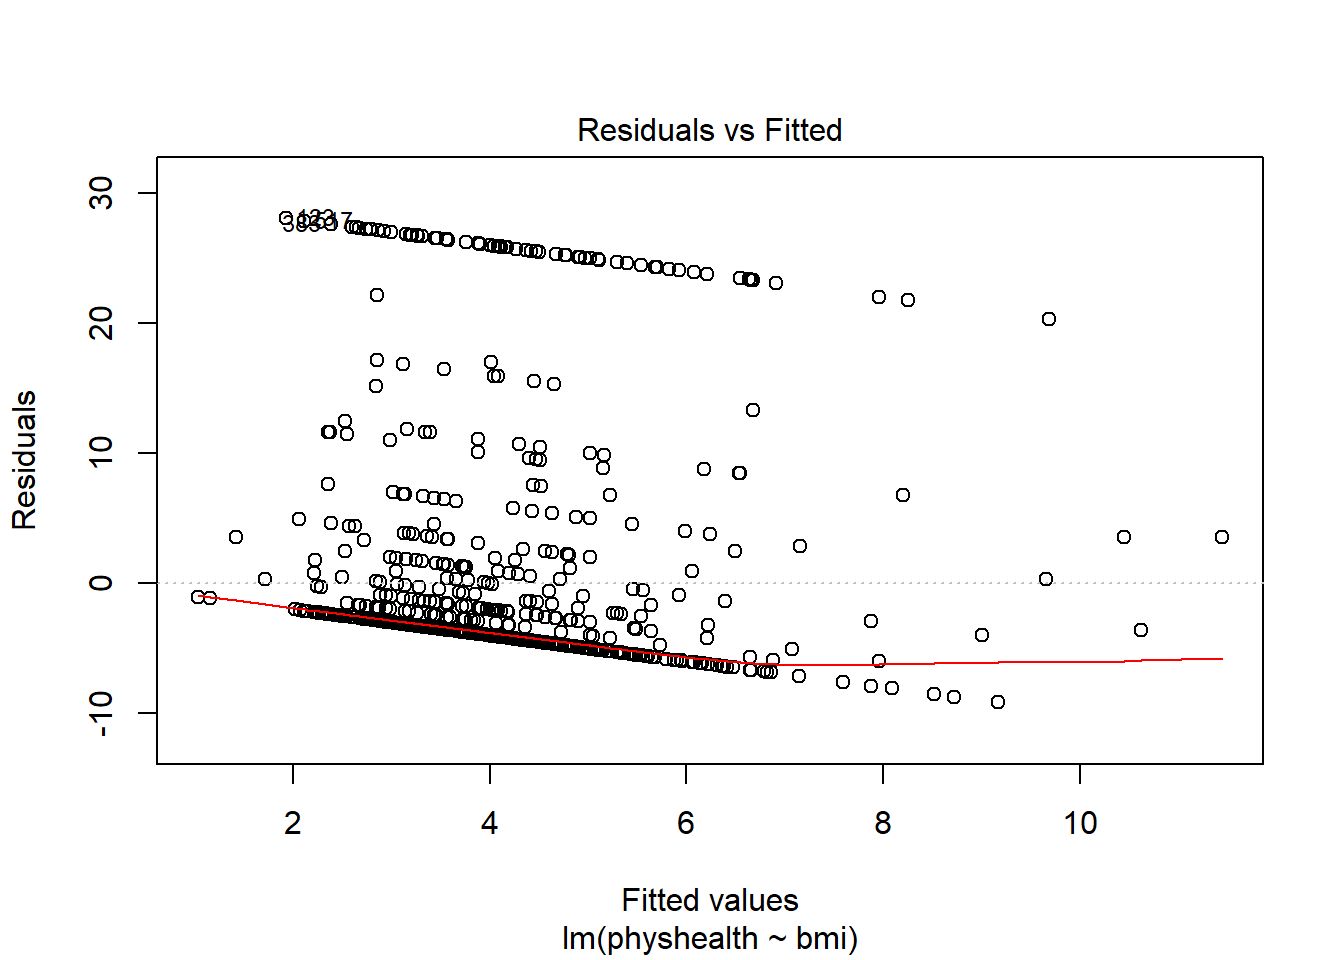
\includegraphics{bookdown-demo_files/figure-latex/chapter2_first_resid_plot_model_A-1.pdf}

This is a plot of residuals vs.~fitted values. The goal here is for this
plot to look like a random scatter of points, perhaps like a ``fuzzy
football'', and that's \textbf{not} what we have. Why?

If you prefer, here's a \texttt{ggplot2} version of a similar plot, now
looking at standardized residuals instead of raw residuals, and adding a
loess smooth and a linear fit to the result.

\begin{Shaded}
\begin{Highlighting}[]
\KeywordTok{ggplot}\NormalTok{(}\KeywordTok{augment}\NormalTok{(model_A), }\KeywordTok{aes}\NormalTok{(}\DataTypeTok{x =}\NormalTok{ .fitted, }\DataTypeTok{y =}\NormalTok{ .std.resid)) }\OperatorTok{+}
\StringTok{    }\KeywordTok{geom_point}\NormalTok{() }\OperatorTok{+}
\StringTok{    }\KeywordTok{geom_smooth}\NormalTok{(}\DataTypeTok{method =} \StringTok{"lm"}\NormalTok{, }\DataTypeTok{se =} \OtherTok{FALSE}\NormalTok{, }\DataTypeTok{col =} \StringTok{"red"}\NormalTok{, }\DataTypeTok{linetype =} \StringTok{"dashed"}\NormalTok{) }\OperatorTok{+}
\StringTok{    }\KeywordTok{geom_smooth}\NormalTok{(}\DataTypeTok{method =} \StringTok{"loess"}\NormalTok{, }\DataTypeTok{se =} \OtherTok{FALSE}\NormalTok{, }\DataTypeTok{col =} \StringTok{"navy"}\NormalTok{) }\OperatorTok{+}
\StringTok{    }\KeywordTok{theme_bw}\NormalTok{()}
\end{Highlighting}
\end{Shaded}

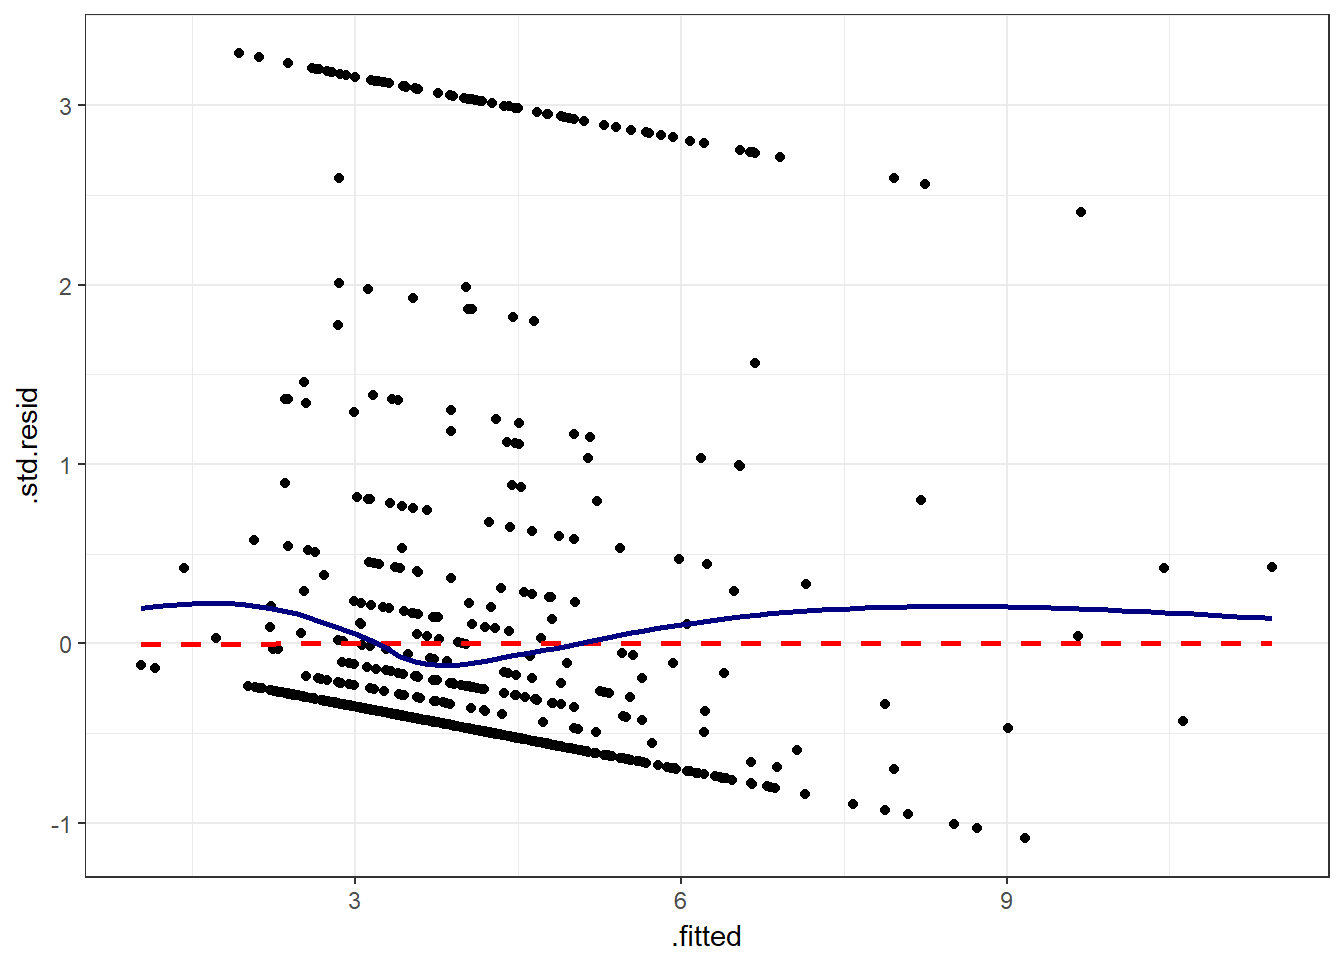
\includegraphics{bookdown-demo_files/figure-latex/chapter2_ggplot_first_resid_plot_model_A-1.pdf}

The problem we're having here becomes, I think, a little more obvious if
we look at what we're predicting. Does \texttt{physhealth} look like a
good candidate for a linear model?

\begin{Shaded}
\begin{Highlighting}[]
\KeywordTok{ggplot}\NormalTok{(smartcle2, }\KeywordTok{aes}\NormalTok{(}\DataTypeTok{x =}\NormalTok{ physhealth)) }\OperatorTok{+}
\KeywordTok{geom_histogram}\NormalTok{(}\DataTypeTok{bins =} \DecValTok{30}\NormalTok{, }\DataTypeTok{fill =} \StringTok{"dodgerblue"}\NormalTok{, }\DataTypeTok{color =} \StringTok{"royalblue"}\NormalTok{)}
\end{Highlighting}
\end{Shaded}

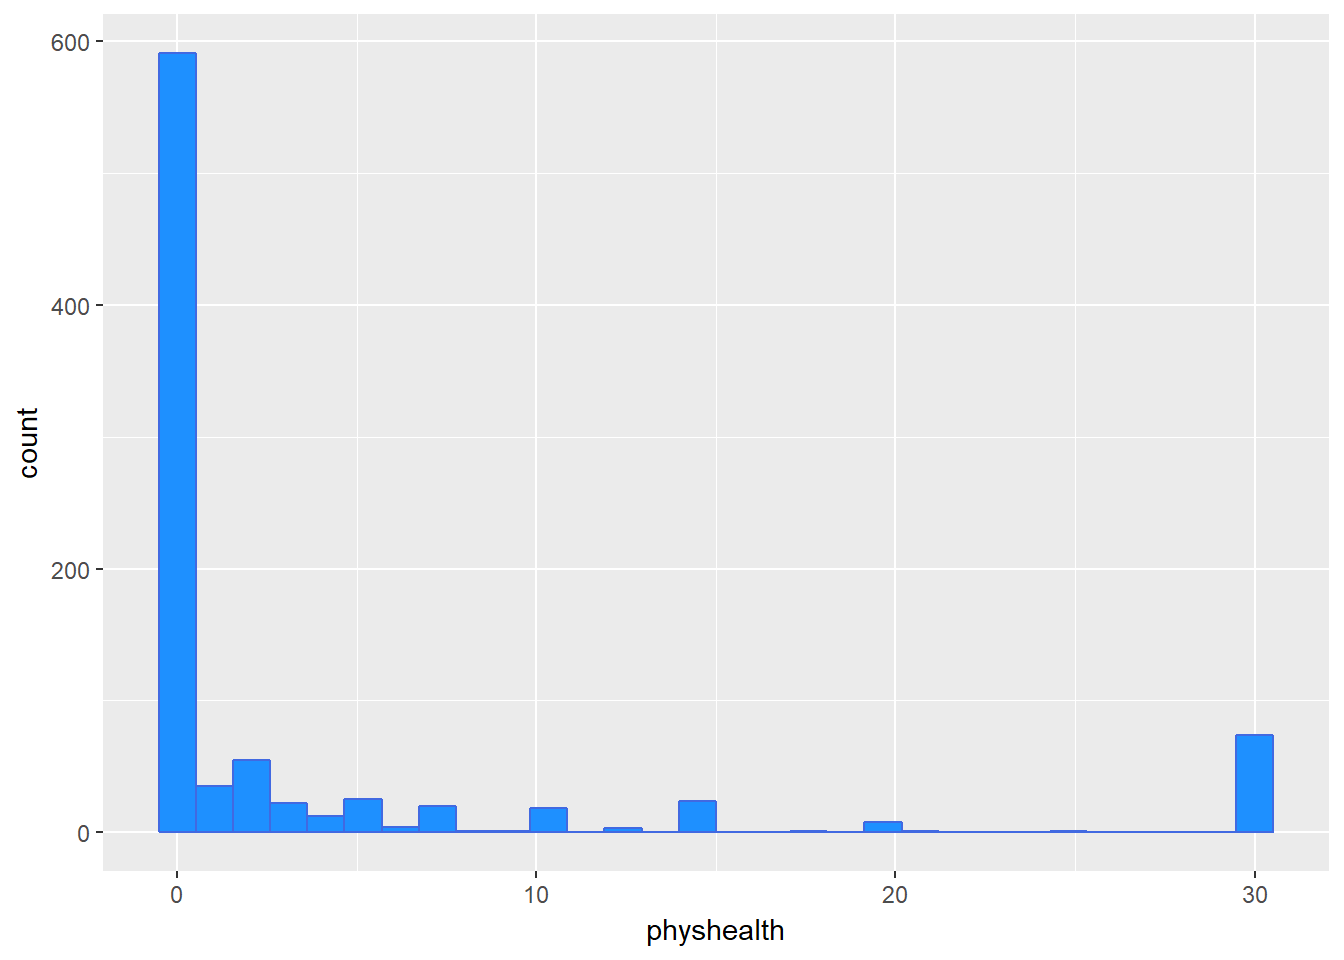
\includegraphics{bookdown-demo_files/figure-latex/histogram_of_physhealth_smartcle2-1.pdf}

\begin{Shaded}
\begin{Highlighting}[]
\NormalTok{smartcle2 }\OperatorTok\StringTok{ }\KeywordTok{count}\NormalTok{(physhealth }\OperatorTok{==}\StringTok{ }\DecValTok{0}\NormalTok{, physhealth }\OperatorTok{==}\StringTok{ }\DecValTok{30}\NormalTok{)}
\end{Highlighting}
\end{Shaded}

\begin{verbatim}
# A tibble: 3 x 3
  `physhealth == 0` `physhealth == 30`     n
  <lgl>             <lgl>              <int>
1 F                 F                    231
2 F                 T                     74
3 T                 F                    591
\end{verbatim}

No matter what model we fit, if we are predicting \texttt{physhealth},
and most of the data are values of 0 and 30, we have limited variation
in our outcome, and so our linear model will be somewhat questionable
just on that basis.

A normal Q-Q plot of the standardized residuals for our
\texttt{model\_A} shows this problem, too.

\begin{Shaded}
\begin{Highlighting}[]
\KeywordTok{plot}\NormalTok{(model_A, }\DataTypeTok{which =} \DecValTok{2}\NormalTok{)}
\end{Highlighting}
\end{Shaded}

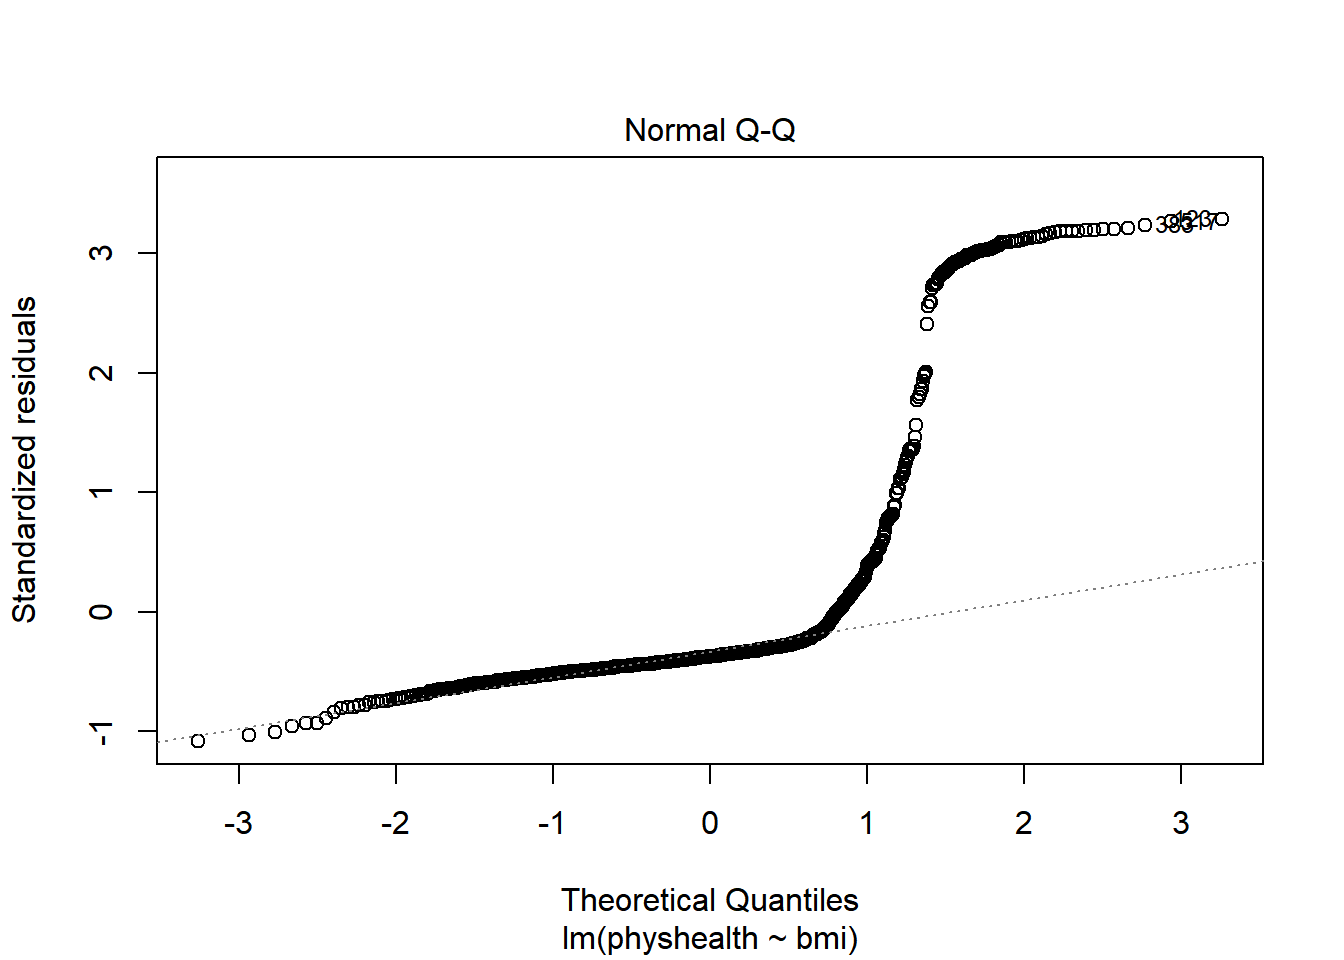
\includegraphics{bookdown-demo_files/figure-latex/chapter2_second_resid_plot_model_A-1.pdf}

We're going to need a method to deal with this sort of outcome, that has
both a floor and a ceiling. We'll get there eventually, but linear
regression alone doesn't look promising.

All right, so that didn't go anywhere great. Let's try again, with a new
outcome.

\section{A New Small Study: Predicting
BMI}\label{a-new-small-study-predicting-bmi}

We'll begin by investigating the problem of predicting \texttt{bmi}, at
first with just three regression inputs: \texttt{sex}, \texttt{exerany}
and \texttt{sleephrs}, in our new \texttt{smartcle2} data set.

\begin{itemize}
\tightlist
\item
  The outcome of interest is \texttt{bmi}.
\item
  Inputs to the regression model are:

  \begin{itemize}
  \tightlist
  \item
    \texttt{female} = 1 if the subject is female, and 0 if they are male
  \item
    \texttt{exerany} = 1 if the subject exercised in the past 30 days,
    and 0 if they didn't
  \item
    \texttt{sleephrs} = hours slept in a typical 24-hour period (treated
    as quantitative)
  \end{itemize}
\end{itemize}

\subsection{\texorpdfstring{Does \texttt{female} predict \texttt{bmi}
well?}{Does female predict bmi well?}}\label{does-female-predict-bmi-well}

\subsubsection{Graphical Assessment}\label{graphical-assessment}

\begin{Shaded}
\begin{Highlighting}[]
\KeywordTok{ggplot}\NormalTok{(smartcle2, }\KeywordTok{aes}\NormalTok{(}\DataTypeTok{x =}\NormalTok{ female, }\DataTypeTok{y =}\NormalTok{ bmi)) }\OperatorTok{+}
\StringTok{    }\KeywordTok{geom_point}\NormalTok{()}
\end{Highlighting}
\end{Shaded}

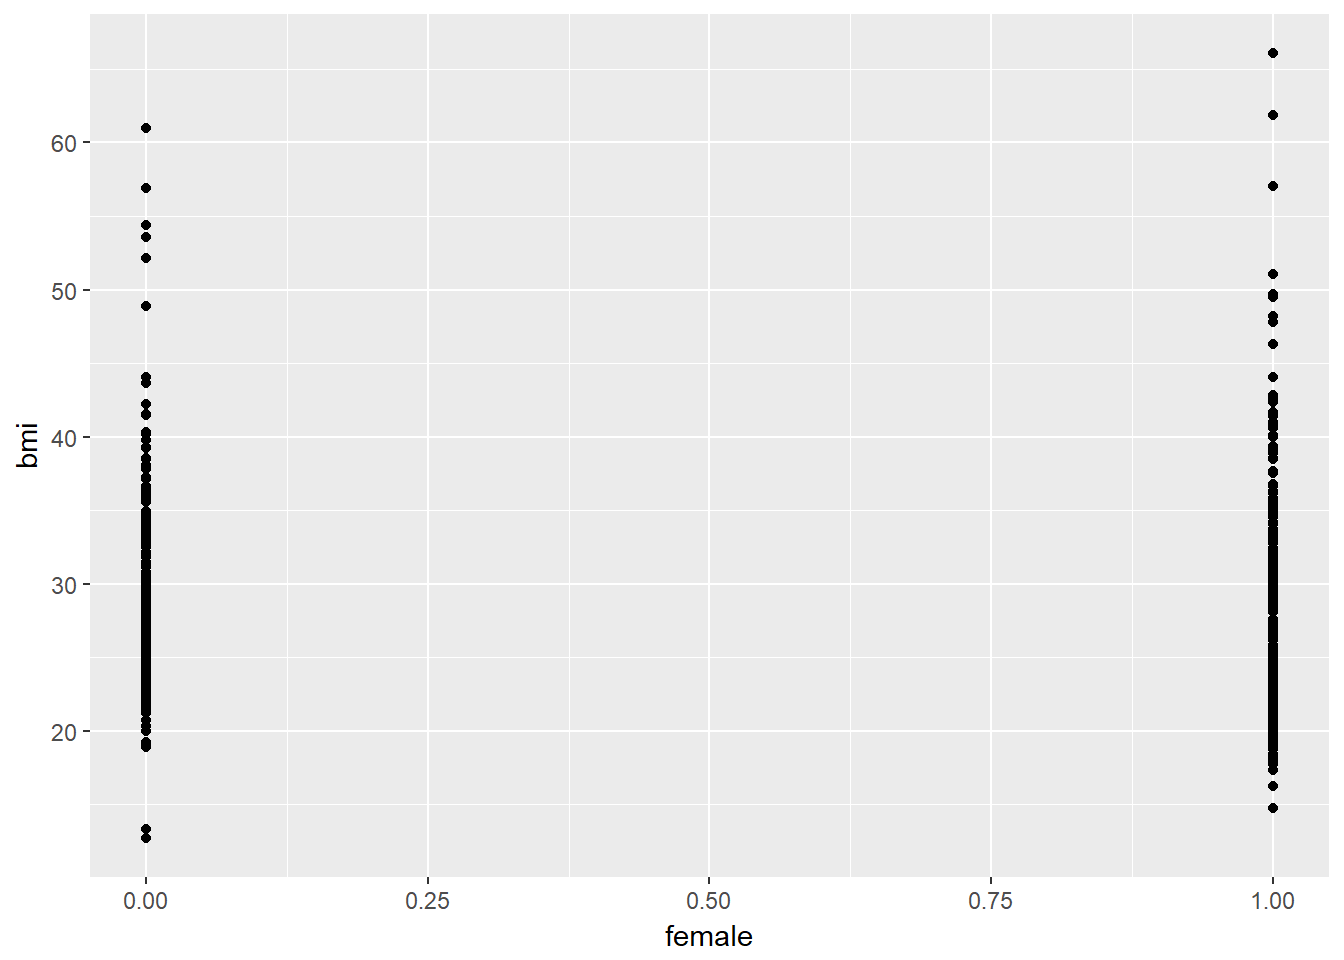
\includegraphics{bookdown-demo_files/figure-latex/c2_sex_bmi_plot1-1.pdf}

Not so helpful. We should probably specify that \texttt{female} is a
factor, and try another plotting approach.

\begin{Shaded}
\begin{Highlighting}[]
\KeywordTok{ggplot}\NormalTok{(smartcle2, }\KeywordTok{aes}\NormalTok{(}\DataTypeTok{x =} \KeywordTok{factor}\NormalTok{(female), }\DataTypeTok{y =}\NormalTok{ bmi)) }\OperatorTok{+}
\StringTok{    }\KeywordTok{geom_boxplot}\NormalTok{()}
\end{Highlighting}
\end{Shaded}

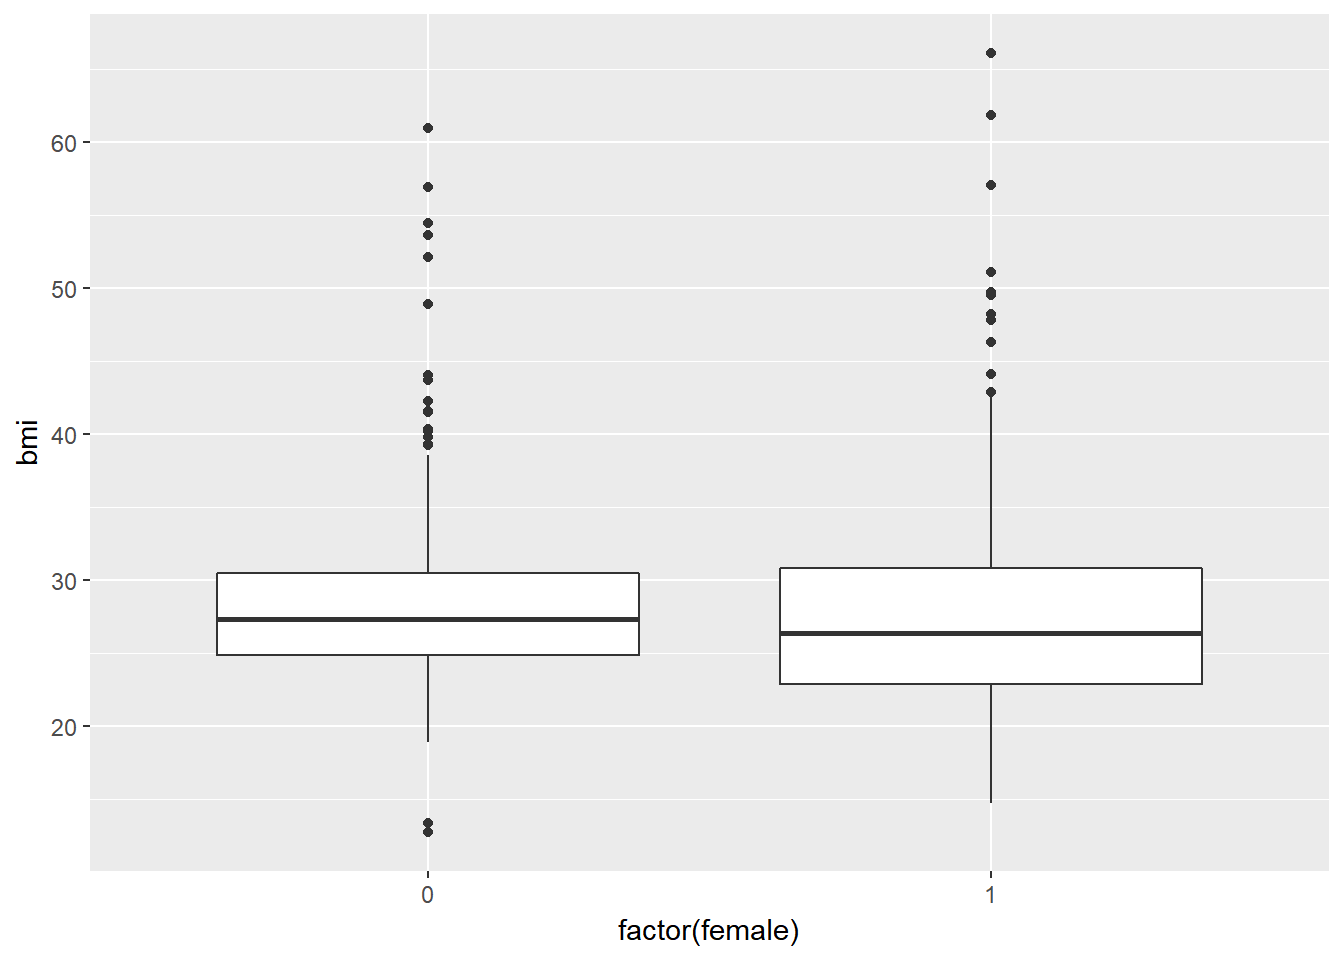
\includegraphics{bookdown-demo_files/figure-latex/c2_sex_bmi_plot2-1.pdf}

The median BMI looks a little higher for males. Let's see if a model
reflects that.

\section{\texorpdfstring{\texttt{c2\_m1}: A simple t-test
model}{c2\_m1: A simple t-test model}}\label{c2_m1-a-simple-t-test-model}

\begin{Shaded}
\begin{Highlighting}[]
\NormalTok{c2_m1 <-}\StringTok{ }\KeywordTok{lm}\NormalTok{(bmi }\OperatorTok{~}\StringTok{ }\NormalTok{female, }\DataTypeTok{data =}\NormalTok{ smartcle2)}
\NormalTok{c2_m1}
\end{Highlighting}
\end{Shaded}

\begin{verbatim}

Call:
lm(formula = bmi ~ female, data = smartcle2)

Coefficients:
(Intercept)       female  
    28.3600      -0.8457  
\end{verbatim}

\begin{Shaded}
\begin{Highlighting}[]
\KeywordTok{summary}\NormalTok{(c2_m1)}
\end{Highlighting}
\end{Shaded}

\begin{verbatim}

Call:
lm(formula = bmi ~ female, data = smartcle2)

Residuals:
    Min      1Q  Median      3Q     Max 
-15.650  -4.129  -1.080   2.727  38.546 

Coefficients:
            Estimate Std. Error t value Pr(>|t|)    
(Intercept)  28.3600     0.3274  86.613   <2e-16 ***
female       -0.8457     0.4282  -1.975   0.0485 *  
---
Signif. codes:  0 '***' 0.001 '**' 0.01 '*' 0.05 '.' 0.1 ' ' 1

Residual standard error: 6.315 on 894 degrees of freedom
Multiple R-squared:  0.004345,  Adjusted R-squared:  0.003231 
F-statistic: 3.902 on 1 and 894 DF,  p-value: 0.04855
\end{verbatim}

\begin{Shaded}
\begin{Highlighting}[]
\KeywordTok{confint}\NormalTok{(c2_m1)}
\end{Highlighting}
\end{Shaded}

\begin{verbatim}
                2.5 %      97.5 %
(Intercept) 27.717372 29.00262801
female      -1.686052 -0.00539878
\end{verbatim}

The model suggests, based on these 896 subjects, that

\begin{itemize}
\tightlist
\item
  our best prediction for males is BMI = 28.36 kg/m\textsuperscript{2},
  and
\item
  our best prediction for females is BMI = 28.36 - 0.85 = 27.51
  kg/m\textsuperscript{2}.
\item
  the mean difference between females and males is -0.85
  kg/m\textsuperscript{2} in BMI
\item
  a 95\% confidence (uncertainty) interval for that mean female - male
  difference in BMI ranges from -1.69 to -0.01
\item
  the model accounts for 0.4\% of the variation in BMI, so that knowing
  the respondent's sex does very little to reduce the size of the
  prediction errors as compared to an intercept only model that would
  predict the overall mean (regardless of sex) for all subjects.
\item
  the model makes some enormous errors, with one subject being predicted
  to have a BMI 38 points lower than his/her actual BMI.
\end{itemize}

Note that this simple regression model just gives us the t-test.

\begin{Shaded}
\begin{Highlighting}[]
\KeywordTok{t.test}\NormalTok{(bmi }\OperatorTok{~}\StringTok{ }\NormalTok{female, }\DataTypeTok{var.equal =} \OtherTok{TRUE}\NormalTok{, }\DataTypeTok{data =}\NormalTok{ smartcle2)}
\end{Highlighting}
\end{Shaded}

\begin{verbatim}

    Two Sample t-test

data:  bmi by female
t = 1.9752, df = 894, p-value = 0.04855
alternative hypothesis: true difference in means is not equal to 0
95 percent confidence interval:
 0.00539878 1.68605160
sample estimates:
mean in group 0 mean in group 1 
       28.36000        27.51427 
\end{verbatim}

\section{\texorpdfstring{\texttt{c2\_m2}: Adding another predictor
(two-way ANOVA without
interaction)}{c2\_m2: Adding another predictor (two-way ANOVA without interaction)}}\label{c2_m2-adding-another-predictor-two-way-anova-without-interaction}

When we add in the information about \texttt{exerany} to our original
model, we might first picture the data. We could look at separate
histograms,

\begin{Shaded}
\begin{Highlighting}[]
\KeywordTok{ggplot}\NormalTok{(smartcle2, }\KeywordTok{aes}\NormalTok{(}\DataTypeTok{x =}\NormalTok{ bmi)) }\OperatorTok{+}
\StringTok{    }\KeywordTok{geom_histogram}\NormalTok{(}\DataTypeTok{bins =} \DecValTok{30}\NormalTok{) }\OperatorTok{+}
\StringTok{    }\KeywordTok{facet_grid}\NormalTok{(female }\OperatorTok{~}\StringTok{ }\NormalTok{exerany, }\DataTypeTok{labeller =}\NormalTok{ label_both)}
\end{Highlighting}
\end{Shaded}

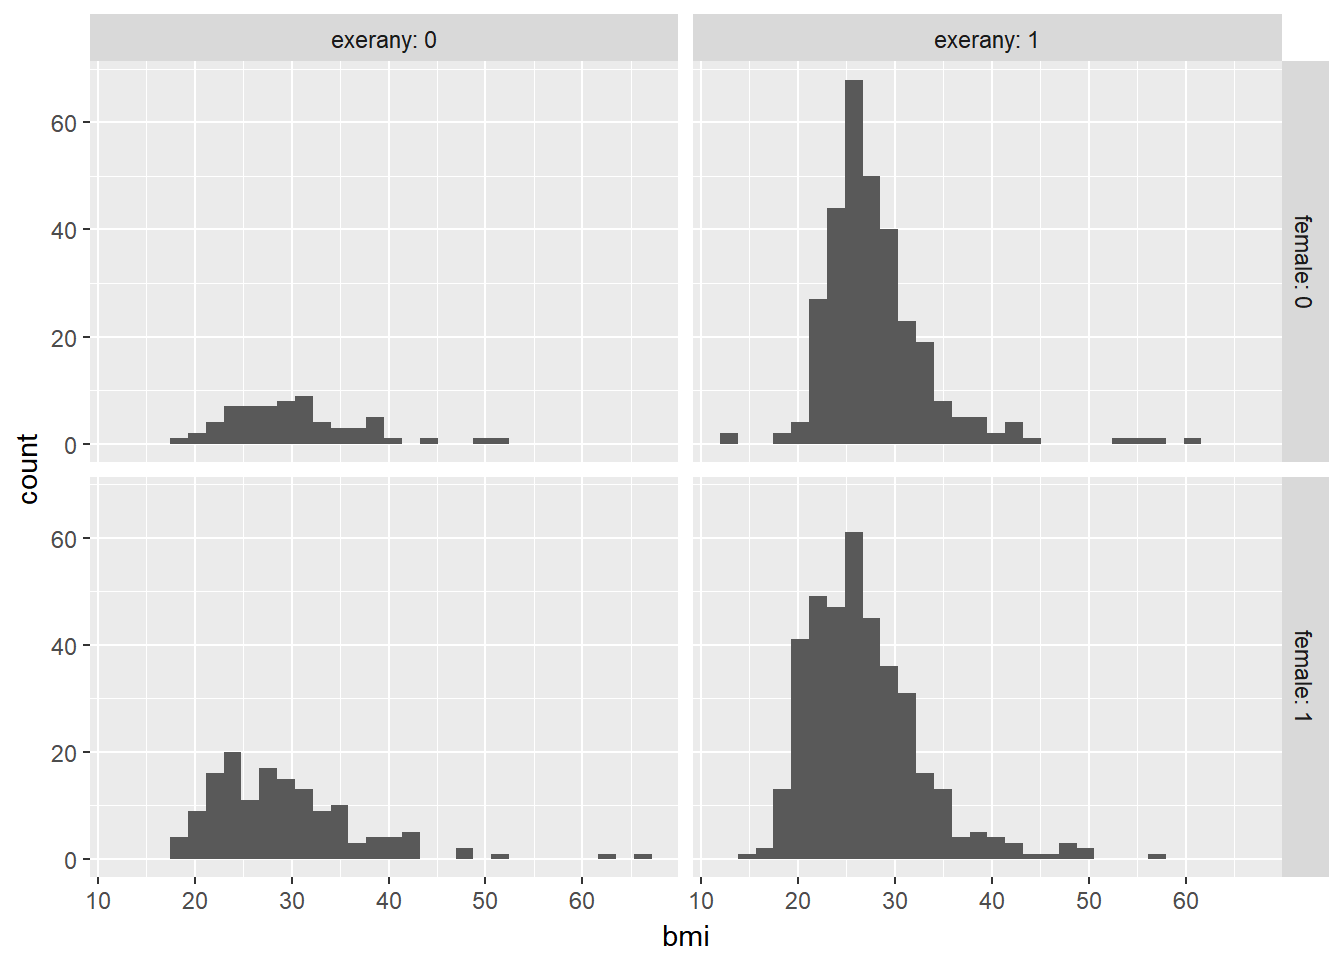
\includegraphics{bookdown-demo_files/figure-latex/c2_smartcle2_plot_bmi_hist_by_female_exerany-1.pdf}

or maybe boxplots?

\begin{Shaded}
\begin{Highlighting}[]
\KeywordTok{ggplot}\NormalTok{(smartcle2, }\KeywordTok{aes}\NormalTok{(}\DataTypeTok{x =} \KeywordTok{factor}\NormalTok{(female), }\DataTypeTok{y =}\NormalTok{ bmi)) }\OperatorTok{+}
\StringTok{    }\KeywordTok{geom_boxplot}\NormalTok{() }\OperatorTok{+}
\StringTok{    }\KeywordTok{facet_wrap}\NormalTok{(}\OperatorTok{~}\StringTok{ }\NormalTok{exerany, }\DataTypeTok{labeller =}\NormalTok{ label_both)}
\end{Highlighting}
\end{Shaded}

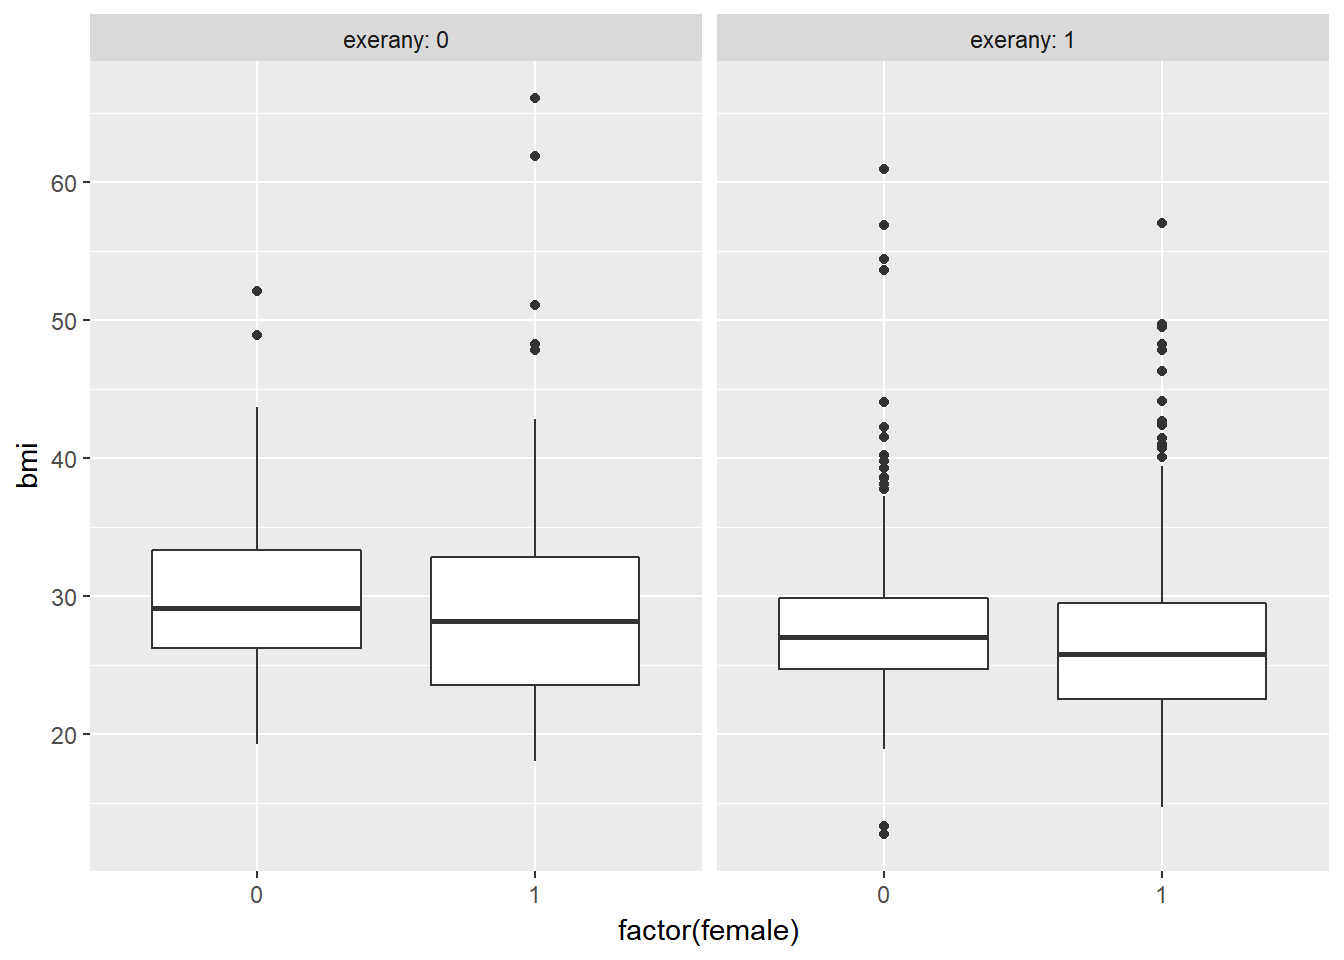
\includegraphics{bookdown-demo_files/figure-latex/c2_smartcle2_plot_bmi_box_by_female_exerany-1.pdf}

\begin{Shaded}
\begin{Highlighting}[]
\KeywordTok{ggplot}\NormalTok{(smartcle2, }\KeywordTok{aes}\NormalTok{(}\DataTypeTok{x =}\NormalTok{ female, }\DataTypeTok{y =}\NormalTok{ bmi))}\OperatorTok{+}
\StringTok{    }\KeywordTok{geom_point}\NormalTok{(}\DataTypeTok{size =} \DecValTok{3}\NormalTok{, }\DataTypeTok{alpha =} \FloatTok{0.2}\NormalTok{) }\OperatorTok{+}
\StringTok{    }\KeywordTok{theme_bw}\NormalTok{() }\OperatorTok{+}
\StringTok{    }\KeywordTok{facet_wrap}\NormalTok{(}\OperatorTok{~}\StringTok{ }\NormalTok{exerany, }\DataTypeTok{labeller =}\NormalTok{ label_both)}
\end{Highlighting}
\end{Shaded}

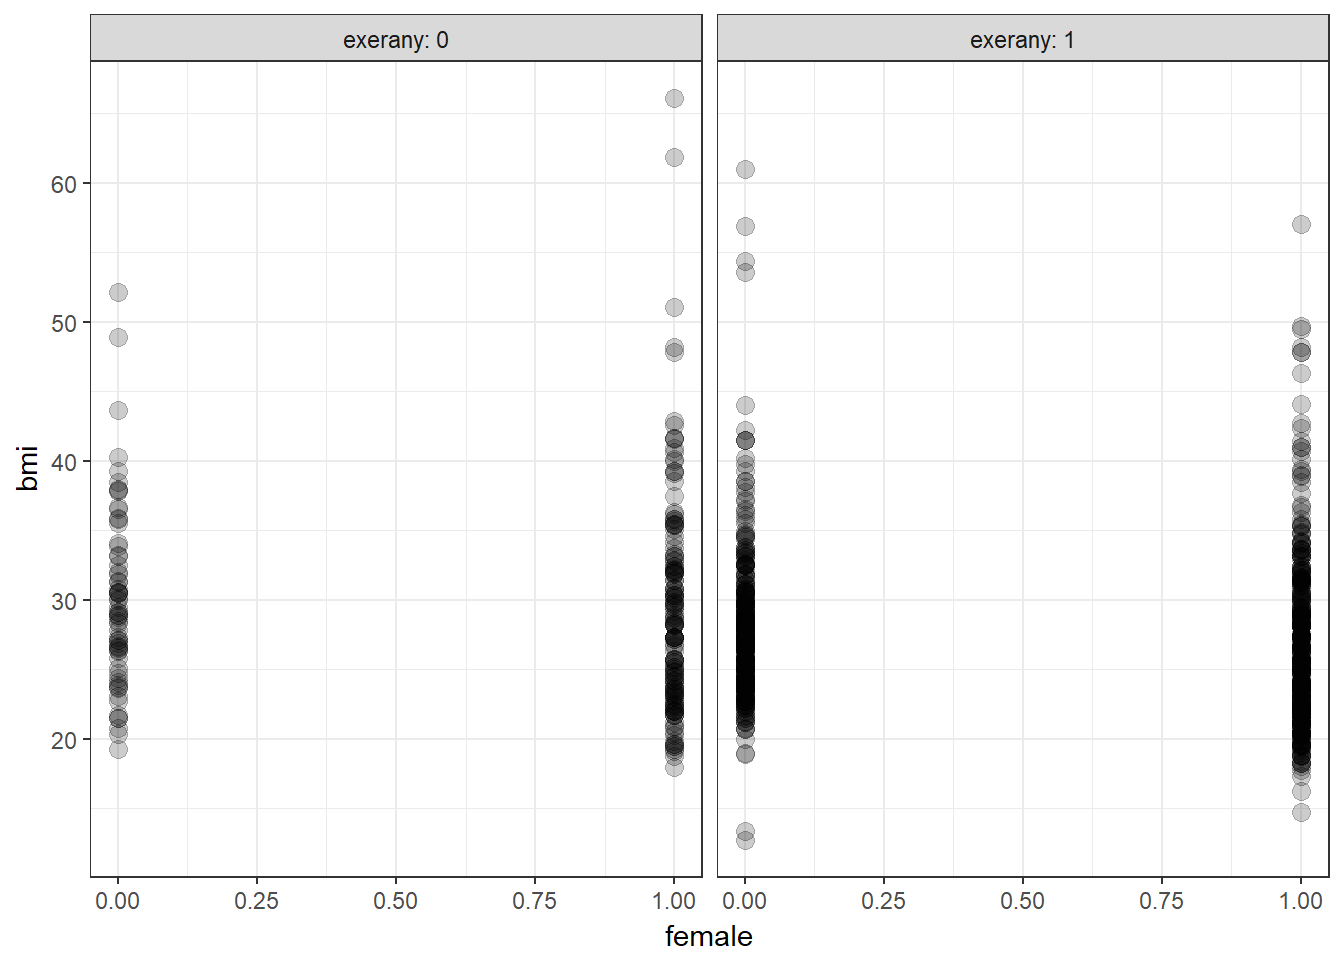
\includegraphics{bookdown-demo_files/figure-latex/c2_smartcle2_plot_bmi_points_by_female_exerany-1.pdf}

OK. Let's try fitting a model.

\begin{Shaded}
\begin{Highlighting}[]
\NormalTok{c2_m2 <-}\StringTok{ }\KeywordTok{lm}\NormalTok{(bmi }\OperatorTok{~}\StringTok{ }\NormalTok{female }\OperatorTok{+}\StringTok{ }\NormalTok{exerany, }\DataTypeTok{data =}\NormalTok{ smartcle2)}
\NormalTok{c2_m2}
\end{Highlighting}
\end{Shaded}

\begin{verbatim}

Call:
lm(formula = bmi ~ female + exerany, data = smartcle2)

Coefficients:
(Intercept)       female      exerany  
     30.334       -1.095       -2.384  
\end{verbatim}

This new model predicts only four predicted values:

\begin{itemize}
\tightlist
\item
  \texttt{bmi} = 30.334 if the subject is male and did not exercise (so
  \texttt{female} = 0 and \texttt{exerany} = 0)
\item
  \texttt{bmi} = 30.334 - 1.095 = 29.239 if the subject is female and
  did not exercise (\texttt{female} = 1 and \texttt{exerany} = 0)
\item
  \texttt{bmi} = 30.334 - 2.384 = 27.950 if the subject is male and
  exercised (so \texttt{female} = 0 and \texttt{exerany} = 1), and,
  finally
\item
  \texttt{bmi} = 30.334 - 1.095 - 2.384 = 26.855 if the subject is
  female and exercised (so both \texttt{female} and \texttt{exerany} =
  1).
\end{itemize}

For those who did not exercise, the model is:

\begin{itemize}
\tightlist
\item
  \texttt{bmi} = 30.334 - 1.095 \texttt{female}
\end{itemize}

and for those who did exercise, the model is:

\begin{itemize}
\tightlist
\item
  \texttt{bmi} = 27.95 - 1.095 \texttt{female}
\end{itemize}

Only the intercept of the \texttt{bmi-female} model changes depending on
\texttt{exerany}.

\begin{Shaded}
\begin{Highlighting}[]
\KeywordTok{summary}\NormalTok{(c2_m2)}
\end{Highlighting}
\end{Shaded}

\begin{verbatim}

Call:
lm(formula = bmi ~ female + exerany, data = smartcle2)

Residuals:
    Min      1Q  Median      3Q     Max 
-15.240  -4.091  -1.095   2.602  36.822 

Coefficients:
            Estimate Std. Error t value Pr(>|t|)    
(Intercept)  30.3335     0.5231   57.99  < 2e-16 ***
female       -1.0952     0.4262   -2.57   0.0103 *  
exerany      -2.3836     0.4965   -4.80 1.86e-06 ***
---
Signif. codes:  0 '***' 0.001 '**' 0.01 '*' 0.05 '.' 0.1 ' ' 1

Residual standard error: 6.239 on 893 degrees of freedom
Multiple R-squared:  0.02939,   Adjusted R-squared:  0.02722 
F-statistic: 13.52 on 2 and 893 DF,  p-value: 1.641e-06
\end{verbatim}

\begin{Shaded}
\begin{Highlighting}[]
\KeywordTok{confint}\NormalTok{(c2_m2)}
\end{Highlighting}
\end{Shaded}

\begin{verbatim}
                2.5 %     97.5 %
(Intercept) 29.306846 31.3602182
female      -1.931629 -0.2588299
exerany     -3.358156 -1.4090777
\end{verbatim}

The slopes of both \texttt{female} and \texttt{exerany} have confidence
intervals that are completely below zero, indicating that both
\texttt{female} sex and \texttt{exerany} appear to be associated with
reductions in \texttt{bmi}.

The R\textsuperscript{2} value suggests that just under 3\% of the
variation in \texttt{bmi} is accounted for by this ANOVA model.

In fact, this regression (on two binary indicator variables) is simply a
two-way ANOVA model without an interaction term.

\begin{Shaded}
\begin{Highlighting}[]
\KeywordTok{anova}\NormalTok{(c2_m2)}
\end{Highlighting}
\end{Shaded}

\begin{verbatim}
Analysis of Variance Table

Response: bmi
           Df Sum Sq Mean Sq F value    Pr(>F)    
female      1    156  155.61  3.9977   0.04586 *  
exerany     1    897  896.93 23.0435 1.856e-06 ***
Residuals 893  34759   38.92                      
---
Signif. codes:  0 '***' 0.001 '**' 0.01 '*' 0.05 '.' 0.1 ' ' 1
\end{verbatim}

\section{\texorpdfstring{\texttt{c2\_m3}: Adding the interaction term
(Two-way ANOVA with
interaction)}{c2\_m3: Adding the interaction term (Two-way ANOVA with interaction)}}\label{c2_m3-adding-the-interaction-term-two-way-anova-with-interaction}

Suppose we want to let the effect of \texttt{female} vary depending on
the \texttt{exerany} status. Then we need to incorporate an interaction
term in our model.

\begin{Shaded}
\begin{Highlighting}[]
\NormalTok{c2_m3 <-}\StringTok{ }\KeywordTok{lm}\NormalTok{(bmi }\OperatorTok{~}\StringTok{ }\NormalTok{female }\OperatorTok{*}\StringTok{ }\NormalTok{exerany, }\DataTypeTok{data =}\NormalTok{ smartcle2)}
\NormalTok{c2_m3}
\end{Highlighting}
\end{Shaded}

\begin{verbatim}

Call:
lm(formula = bmi ~ female * exerany, data = smartcle2)

Coefficients:
   (Intercept)          female         exerany  female:exerany  
       30.1359         -0.8104         -2.1450         -0.3592  
\end{verbatim}

So, for example, for a male who exercises, this model predicts

\begin{itemize}
\tightlist
\item
  \texttt{bmi} = 30.136 - 0.810 (0) - 2.145 (1) - 0.359 (0)(1) = 30.136
  - 2.145 = 27.991
\end{itemize}

And for a female who exercises, the model predicts

\begin{itemize}
\tightlist
\item
  \texttt{bmi} = 30.136 - 0.810 (1) - 2.145 (1) - 0.359 (1)(1) = 30.136
  - 0.810 - 2.145 - 0.359 = 26.822
\end{itemize}

For those who did not exercise, the model is:

\begin{itemize}
\tightlist
\item
  \texttt{bmi} = 30.136 - 0.81 \texttt{female}
\end{itemize}

But for those who did exercise, the model is:

\begin{itemize}
\tightlist
\item
  \texttt{bmi} = (30.136 - 2.145) + (-0.810 + (-0.359)) \texttt{female},
  or ,,,
\item
  \texttt{bmi} = 27.991 - 1.169 \texttt{female}
\end{itemize}

Now, both the slope and the intercept of the \texttt{bmi-female} model
change depending on \texttt{exerany}.

\begin{Shaded}
\begin{Highlighting}[]
\KeywordTok{summary}\NormalTok{(c2_m3)}
\end{Highlighting}
\end{Shaded}

\begin{verbatim}

Call:
lm(formula = bmi ~ female * exerany, data = smartcle2)

Residuals:
    Min      1Q  Median      3Q     Max 
-15.281  -4.101  -1.061   2.566  36.734 

Coefficients:
               Estimate Std. Error t value Pr(>|t|)    
(Intercept)     30.1359     0.7802  38.624   <2e-16 ***
female          -0.8104     0.9367  -0.865   0.3872    
exerany         -2.1450     0.8575  -2.501   0.0125 *  
female:exerany  -0.3592     1.0520  -0.341   0.7328    
---
Signif. codes:  0 '***' 0.001 '**' 0.01 '*' 0.05 '.' 0.1 ' ' 1

Residual standard error: 6.242 on 892 degrees of freedom
Multiple R-squared:  0.02952,   Adjusted R-squared:  0.02625 
F-statistic: 9.044 on 3 and 892 DF,  p-value: 6.669e-06
\end{verbatim}

\begin{Shaded}
\begin{Highlighting}[]
\KeywordTok{confint}\NormalTok{(c2_m3)}
\end{Highlighting}
\end{Shaded}

\begin{verbatim}
                   2.5 %     97.5 %
(Intercept)    28.604610 31.6672650
female         -2.648893  1.0280526
exerany        -3.827886 -0.4620407
female:exerany -2.423994  1.7055248
\end{verbatim}

In fact, this regression (on two binary indicator variables and a
product term) is simply a two-way ANOVA model with an interaction term.

\begin{Shaded}
\begin{Highlighting}[]
\KeywordTok{anova}\NormalTok{(c2_m3)}
\end{Highlighting}
\end{Shaded}

\begin{verbatim}
Analysis of Variance Table

Response: bmi
                Df Sum Sq Mean Sq F value    Pr(>F)    
female           1    156  155.61  3.9938   0.04597 *  
exerany          1    897  896.93 23.0207 1.878e-06 ***
female:exerany   1      5    4.54  0.1166   0.73283    
Residuals      892  34754   38.96                      
---
Signif. codes:  0 '***' 0.001 '**' 0.01 '*' 0.05 '.' 0.1 ' ' 1
\end{verbatim}

The interaction term doesn't change very much here. Its uncertainty
interval includes zero, and the overall model still accounts for just
under 3\% of the variation in \texttt{bmi}.

\section{\texorpdfstring{\texttt{c2\_m4}: Using \texttt{female} and
\texttt{sleephrs} in a model for
\texttt{bmi}}{c2\_m4: Using female and sleephrs in a model for bmi}}\label{c2_m4-using-female-and-sleephrs-in-a-model-for-bmi}

\begin{Shaded}
\begin{Highlighting}[]
\KeywordTok{ggplot}\NormalTok{(smartcle2, }\KeywordTok{aes}\NormalTok{(}\DataTypeTok{x =}\NormalTok{ sleephrs, }\DataTypeTok{y =}\NormalTok{ bmi, }\DataTypeTok{color =} \KeywordTok{factor}\NormalTok{(female))) }\OperatorTok{+}
\StringTok{    }\KeywordTok{geom_point}\NormalTok{() }\OperatorTok{+}\StringTok{ }
\StringTok{    }\KeywordTok{guides}\NormalTok{(}\DataTypeTok{col =} \OtherTok{FALSE}\NormalTok{) }\OperatorTok{+}
\StringTok{    }\KeywordTok{geom_smooth}\NormalTok{(}\DataTypeTok{method =} \StringTok{"lm"}\NormalTok{, }\DataTypeTok{se =} \OtherTok{FALSE}\NormalTok{) }\OperatorTok{+}
\StringTok{    }\KeywordTok{facet_wrap}\NormalTok{(}\OperatorTok{~}\StringTok{ }\NormalTok{female, }\DataTypeTok{labeller =}\NormalTok{ label_both) }
\end{Highlighting}
\end{Shaded}

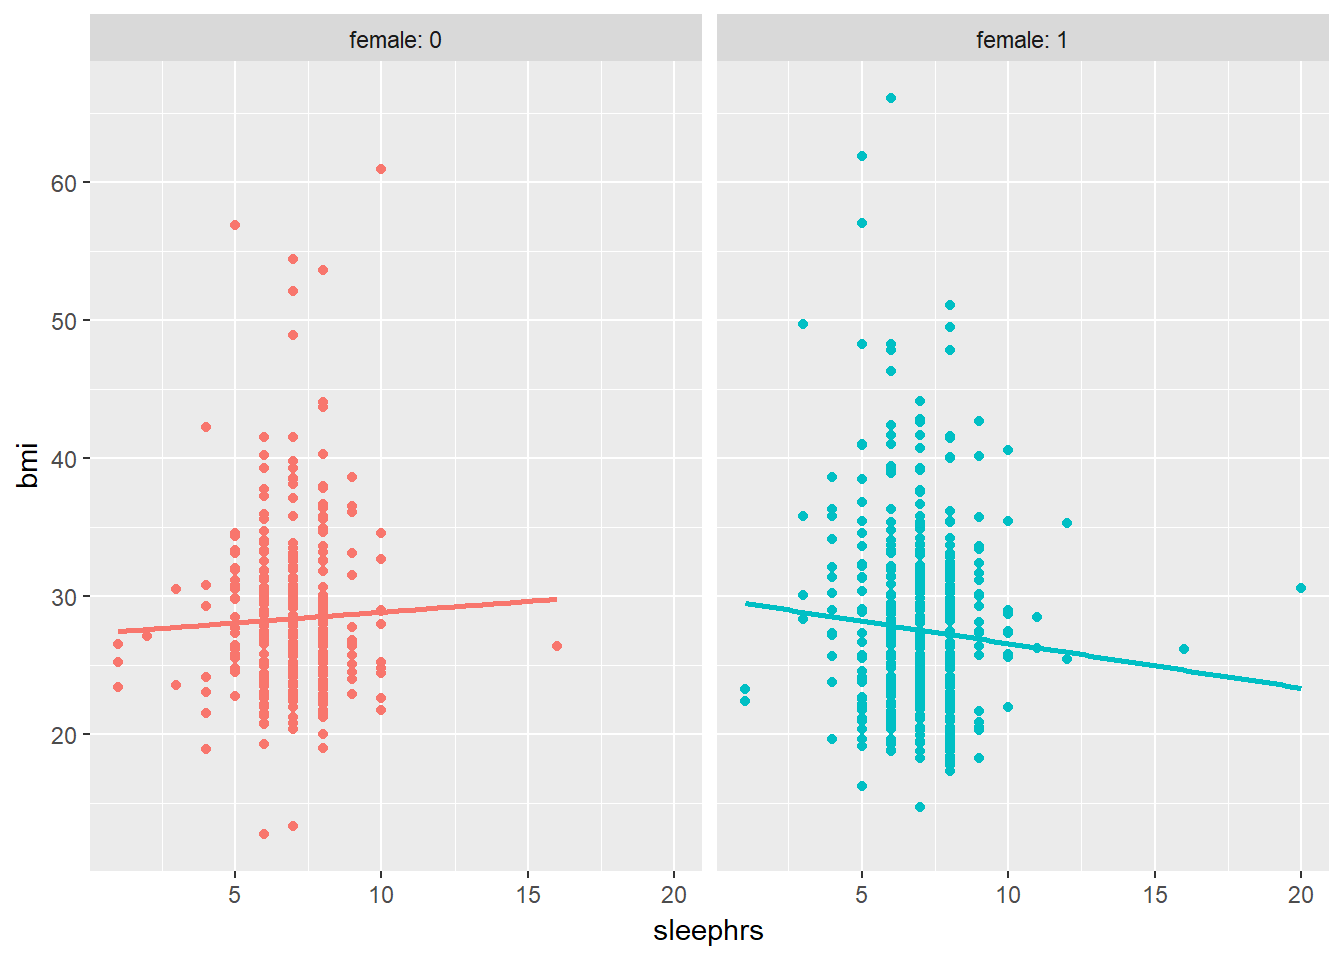
\includegraphics{bookdown-demo_files/figure-latex/graph_to_set_up_c2_m4-1.pdf}

Does the difference in slopes of \texttt{bmi} and \texttt{sleephrs} for
males and females appear to be substantial and important?

\begin{Shaded}
\begin{Highlighting}[]
\NormalTok{c2_m4 <-}\StringTok{ }\KeywordTok{lm}\NormalTok{(bmi }\OperatorTok{~}\StringTok{ }\NormalTok{female }\OperatorTok{*}\StringTok{ }\NormalTok{sleephrs, }\DataTypeTok{data =}\NormalTok{ smartcle2)}

\KeywordTok{summary}\NormalTok{(c2_m4)}
\end{Highlighting}
\end{Shaded}

\begin{verbatim}

Call:
lm(formula = bmi ~ female * sleephrs, data = smartcle2)

Residuals:
    Min      1Q  Median      3Q     Max 
-15.498  -4.179  -1.035   2.830  38.204 

Coefficients:
                Estimate Std. Error t value Pr(>|t|)    
(Intercept)      27.2661     1.6320  16.707   <2e-16 ***
female            2.5263     2.0975   1.204    0.229    
sleephrs          0.1569     0.2294   0.684    0.494    
female:sleephrs  -0.4797     0.2931  -1.636    0.102    
---
Signif. codes:  0 '***' 0.001 '**' 0.01 '*' 0.05 '.' 0.1 ' ' 1

Residual standard error: 6.31 on 892 degrees of freedom
Multiple R-squared:  0.008341,  Adjusted R-squared:  0.005006 
F-statistic: 2.501 on 3 and 892 DF,  p-value: 0.05818
\end{verbatim}

Does it seem as though the addition of \texttt{sleephrs} has improved
our model substantially over a model with \texttt{female} alone (which,
you recall, was \texttt{c2\_m1})?

Since the \texttt{c2\_m4} model contains the \texttt{c2\_m1} model's
predictors as a subset and the outcome is the same for each model, we
consider the models \emph{nested} and have some extra tools available to
compare them.

\begin{itemize}
\tightlist
\item
  I might start by looking at the basic summaries for each model.
\end{itemize}

\begin{Shaded}
\begin{Highlighting}[]
\KeywordTok{glance}\NormalTok{(c2_m4)}
\end{Highlighting}
\end{Shaded}

\begin{verbatim}
    r.squared adj.r.squared    sigma statistic    p.value df    logLik
1 0.008341404   0.005006229 6.309685   2.50104 0.05818038  4 -2919.873
       AIC      BIC deviance df.residual
1 5849.747 5873.736 35512.42         892
\end{verbatim}

\begin{Shaded}
\begin{Highlighting}[]
\KeywordTok{glance}\NormalTok{(c2_m1)}
\end{Highlighting}
\end{Shaded}

\begin{verbatim}
    r.squared adj.r.squared   sigma statistic    p.value df    logLik
1 0.004345169   0.003231461 6.31531  3.901534 0.04854928  2 -2921.675
      AIC      BIC deviance df.residual
1 5849.35 5863.744 35655.53         894
\end{verbatim}

\begin{itemize}
\tightlist
\item
  The R\textsuperscript{2} is twice as large for the model with
  \texttt{sleephrs}, but still very tiny.
\item
  The \emph{p} value for the global ANOVA test is actually less
  significant in \texttt{c2\_m4} than in \texttt{c2\_m1}.
\item
  Smaller AIC and smaller BIC statistics are more desirable. Here,
  there's little to choose from, but \texttt{c2\_m1} is a little better
  on each standard.
\item
  We might also consider a significance test by looking at an ANOVA
  model comparison. This is only appropriate because \texttt{c2\_m1} is
  nested in \texttt{c2\_m4}.
\end{itemize}

\begin{Shaded}
\begin{Highlighting}[]
\KeywordTok{anova}\NormalTok{(c2_m4, c2_m1)}
\end{Highlighting}
\end{Shaded}

\begin{verbatim}
Analysis of Variance Table

Model 1: bmi ~ female * sleephrs
Model 2: bmi ~ female
  Res.Df   RSS Df Sum of Sq      F Pr(>F)
1    892 35512                           
2    894 35656 -2   -143.11 1.7973 0.1663
\end{verbatim}

The addition of the \texttt{sleephrs} term picked up 143 in the sum of
squares column, at a cost of two degrees of freedom, yielding a \emph{p}
value of 0.166, suggesting that this isn't a significant improvement
over the model that just did a t-test on \texttt{female}.

\section{\texorpdfstring{\texttt{c2\_m5}: What if we add more
variables?}{c2\_m5: What if we add more variables?}}\label{c2_m5-what-if-we-add-more-variables}

We can boost our R\textsuperscript{2} a bit, to over 5\%, by adding in
two new variables, related to whether or not the subject (in the past 30
days) used the internet, and on how many days the subject drank
alcoholic beverages.

\begin{Shaded}
\begin{Highlighting}[]
\NormalTok{c2_m5 <-}\StringTok{ }\KeywordTok{lm}\NormalTok{(bmi }\OperatorTok{~}\StringTok{ }\NormalTok{female }\OperatorTok{+}\StringTok{ }\NormalTok{exerany }\OperatorTok{+}\StringTok{ }\NormalTok{sleephrs }\OperatorTok{+}\StringTok{ }\NormalTok{internet30 }\OperatorTok{+}\StringTok{ }\NormalTok{alcdays,}
         \DataTypeTok{data =}\NormalTok{ smartcle2)}
\KeywordTok{summary}\NormalTok{(c2_m5)}
\end{Highlighting}
\end{Shaded}

\begin{verbatim}

Call:
lm(formula = bmi ~ female + exerany + sleephrs + internet30 + 
    alcdays, data = smartcle2)

Residuals:
    Min      1Q  Median      3Q     Max 
-16.147  -3.997  -0.856   2.487  35.965 

Coefficients:
            Estimate Std. Error t value Pr(>|t|)    
(Intercept) 30.84066    1.18458  26.035  < 2e-16 ***
female      -1.28801    0.42805  -3.009   0.0027 ** 
exerany     -2.42161    0.49853  -4.858 1.40e-06 ***
sleephrs    -0.14118    0.13988  -1.009   0.3131    
internet30   1.38916    0.54252   2.561   0.0106 *  
alcdays     -0.10460    0.02595  -4.030 6.04e-05 ***
---
Signif. codes:  0 '***' 0.001 '**' 0.01 '*' 0.05 '.' 0.1 ' ' 1

Residual standard error: 6.174 on 890 degrees of freedom
Multiple R-squared:  0.05258,   Adjusted R-squared:  0.04726 
F-statistic: 9.879 on 5 and 890 DF,  p-value: 3.304e-09
\end{verbatim}

\begin{enumerate}
\def\labelenumi{\arabic{enumi}.}
\tightlist
\item
  Here's the ANOVA for this model. What can we study with this?
\end{enumerate}

\begin{Shaded}
\begin{Highlighting}[]
\KeywordTok{anova}\NormalTok{(c2_m5)}
\end{Highlighting}
\end{Shaded}

\begin{verbatim}
Analysis of Variance Table

Response: bmi
            Df Sum Sq Mean Sq F value    Pr(>F)    
female       1    156  155.61  4.0818   0.04365 *  
exerany      1    897  896.93 23.5283 1.453e-06 ***
sleephrs     1     33   32.90  0.8631   0.35313    
internet30   1    178  178.33  4.6779   0.03082 *  
alcdays      1    619  619.26 16.2443 6.044e-05 ***
Residuals  890  33928   38.12                      
---
Signif. codes:  0 '***' 0.001 '**' 0.01 '*' 0.05 '.' 0.1 ' ' 1
\end{verbatim}

\begin{enumerate}
\def\labelenumi{\arabic{enumi}.}
\setcounter{enumi}{1}
\tightlist
\item
  Consider the revised output below. Now what can we study?
\end{enumerate}

\begin{Shaded}
\begin{Highlighting}[]
\KeywordTok{anova}\NormalTok{(}\KeywordTok{lm}\NormalTok{(bmi }\OperatorTok{~}\StringTok{ }\NormalTok{exerany }\OperatorTok{+}\StringTok{ }\NormalTok{internet30 }\OperatorTok{+}\StringTok{ }\NormalTok{alcdays }\OperatorTok{+}\StringTok{ }\NormalTok{female }\OperatorTok{+}\StringTok{ }\NormalTok{sleephrs,}
         \DataTypeTok{data =}\NormalTok{ smartcle2))}
\end{Highlighting}
\end{Shaded}

\begin{verbatim}
Analysis of Variance Table

Response: bmi
            Df Sum Sq Mean Sq F value    Pr(>F)    
exerany      1    795  795.46 20.8664 5.618e-06 ***
internet30   1    212  211.95  5.5599 0.0185925 *  
alcdays      1    486  486.03 12.7496 0.0003752 ***
female       1    351  350.75  9.2010 0.0024891 ** 
sleephrs     1     39   38.83  1.0186 0.3131176    
Residuals  890  33928   38.12                      
---
Signif. codes:  0 '***' 0.001 '**' 0.01 '*' 0.05 '.' 0.1 ' ' 1
\end{verbatim}

\begin{enumerate}
\def\labelenumi{\arabic{enumi}.}
\setcounter{enumi}{2}
\tightlist
\item
  What does the output below let us conclude?
\end{enumerate}

\begin{Shaded}
\begin{Highlighting}[]
\KeywordTok{anova}\NormalTok{(}\KeywordTok{lm}\NormalTok{(bmi }\OperatorTok{~}\StringTok{ }\NormalTok{exerany }\OperatorTok{+}\StringTok{ }\NormalTok{internet30 }\OperatorTok{+}\StringTok{ }\NormalTok{alcdays }\OperatorTok{+}\StringTok{ }\NormalTok{female }\OperatorTok{+}\StringTok{ }\NormalTok{sleephrs, }
         \DataTypeTok{data =}\NormalTok{ smartcle2),}
      \KeywordTok{lm}\NormalTok{(bmi }\OperatorTok{~}\StringTok{ }\NormalTok{exerany }\OperatorTok{+}\StringTok{ }\NormalTok{female }\OperatorTok{+}\StringTok{ }\NormalTok{alcdays, }
         \DataTypeTok{data =}\NormalTok{ smartcle2))}
\end{Highlighting}
\end{Shaded}

\begin{verbatim}
Analysis of Variance Table

Model 1: bmi ~ exerany + internet30 + alcdays + female + sleephrs
Model 2: bmi ~ exerany + female + alcdays
  Res.Df   RSS Df Sum of Sq      F  Pr(>F)  
1    890 33928                              
2    892 34221 -2    -293.2 3.8456 0.02173 *
---
Signif. codes:  0 '***' 0.001 '**' 0.01 '*' 0.05 '.' 0.1 ' ' 1
\end{verbatim}

\begin{enumerate}
\def\labelenumi{\arabic{enumi}.}
\setcounter{enumi}{3}
\tightlist
\item
  What does it mean for the models to be ``nested''?
\end{enumerate}

\section{\texorpdfstring{\texttt{c2\_m6}: Would adding self-reported
health
help?}{c2\_m6: Would adding self-reported health help?}}\label{c2_m6-would-adding-self-reported-health-help}

And we can do even a bit better than that by adding in a
multi-categorical measure: self-reported general health.

\begin{Shaded}
\begin{Highlighting}[]
\NormalTok{c2_m6 <-}\StringTok{ }\KeywordTok{lm}\NormalTok{(bmi }\OperatorTok{~}\StringTok{ }\NormalTok{female }\OperatorTok{+}\StringTok{ }\NormalTok{exerany }\OperatorTok{+}\StringTok{ }\NormalTok{sleephrs }\OperatorTok{+}\StringTok{ }\NormalTok{internet30 }\OperatorTok{+}\StringTok{ }\NormalTok{alcdays }\OperatorTok{+}\StringTok{ }\NormalTok{genhealth,}
         \DataTypeTok{data =}\NormalTok{ smartcle2)}
\KeywordTok{summary}\NormalTok{(c2_m6)}
\end{Highlighting}
\end{Shaded}

\begin{verbatim}

Call:
lm(formula = bmi ~ female + exerany + sleephrs + internet30 + 
    alcdays + genhealth, data = smartcle2)

Residuals:
    Min      1Q  Median      3Q     Max 
-16.331  -3.813  -0.838   2.679  34.166 

Coefficients:
                    Estimate Std. Error t value Pr(>|t|)    
(Intercept)         26.49498    1.31121  20.206  < 2e-16 ***
female              -0.85520    0.41969  -2.038 0.041879 *  
exerany             -1.61968    0.50541  -3.205 0.001400 ** 
sleephrs            -0.12719    0.13613  -0.934 0.350368    
internet30           2.02498    0.53898   3.757 0.000183 ***
alcdays             -0.08431    0.02537  -3.324 0.000925 ***
genhealth2_VeryGood  2.10537    0.59408   3.544 0.000415 ***
genhealth3_Good      4.08245    0.60739   6.721 3.22e-11 ***
genhealth4_Fair      4.99213    0.80178   6.226 7.37e-10 ***
genhealth5_Poor      3.11025    1.12614   2.762 0.005866 ** 
---
Signif. codes:  0 '***' 0.001 '**' 0.01 '*' 0.05 '.' 0.1 ' ' 1

Residual standard error: 5.993 on 886 degrees of freedom
Multiple R-squared:  0.1115,    Adjusted R-squared:  0.1024 
F-statistic: 12.35 on 9 and 886 DF,  p-value: < 2.2e-16
\end{verbatim}

\begin{enumerate}
\def\labelenumi{\arabic{enumi}.}
\item
  If Harry and Marty have the same values of \texttt{female},
  \texttt{exerany}, \texttt{sleephrs}, \texttt{internet30} and
  \texttt{alcdays}, but Harry rates his health as Good, and Marty rates
  his as Fair, then what is the difference in the predictions? Who is
  predicted to have a larger BMI, and by how much?
\item
  What does this normal probability plot of the residuals suggest?
\end{enumerate}

\begin{Shaded}
\begin{Highlighting}[]
\KeywordTok{plot}\NormalTok{(c2_m6, }\DataTypeTok{which =} \DecValTok{2}\NormalTok{)}
\end{Highlighting}
\end{Shaded}

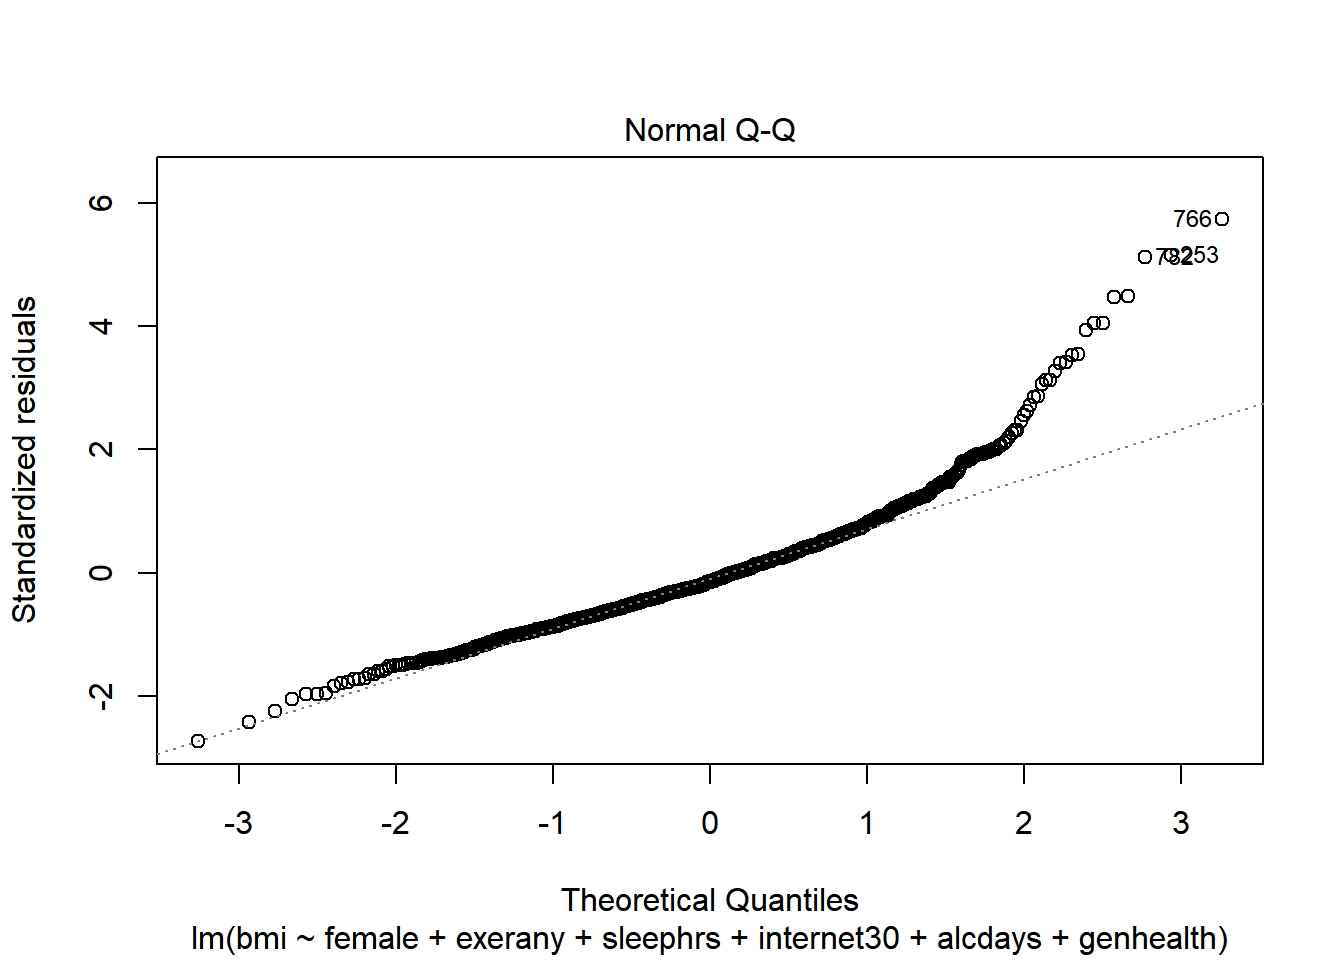
\includegraphics{bookdown-demo_files/figure-latex/c2_m6_residuals_normality-1.pdf}

\section{\texorpdfstring{\texttt{c2\_m7}: What if we added days of work
missed?}{c2\_m7: What if we added days of work missed?}}\label{c2_m7-what-if-we-added-days-of-work-missed}

\begin{Shaded}
\begin{Highlighting}[]
\NormalTok{c2_m7 <-}\StringTok{ }\KeywordTok{lm}\NormalTok{(bmi }\OperatorTok{~}\StringTok{ }\NormalTok{female }\OperatorTok{+}\StringTok{ }\NormalTok{exerany }\OperatorTok{+}\StringTok{ }\NormalTok{sleephrs }\OperatorTok{+}\StringTok{ }\NormalTok{internet30 }\OperatorTok{+}\StringTok{ }\NormalTok{alcdays }\OperatorTok{+}\StringTok{ }
\StringTok{                }\NormalTok{genhealth }\OperatorTok{+}\StringTok{ }\NormalTok{physhealth }\OperatorTok{+}\StringTok{ }\NormalTok{menthealth,}
         \DataTypeTok{data =}\NormalTok{ smartcle2)}
\KeywordTok{summary}\NormalTok{(c2_m7)}
\end{Highlighting}
\end{Shaded}

\begin{verbatim}

Call:
lm(formula = bmi ~ female + exerany + sleephrs + internet30 + 
    alcdays + genhealth + physhealth + menthealth, data = smartcle2)

Residuals:
    Min      1Q  Median      3Q     Max 
-16.060  -3.804  -0.890   2.794  33.972 

Coefficients:
                    Estimate Std. Error t value Pr(>|t|)    
(Intercept)         25.88208    1.31854  19.629  < 2e-16 ***
female              -0.96435    0.41908  -2.301 0.021616 *  
exerany             -1.43171    0.50635  -2.828 0.004797 ** 
sleephrs            -0.08033    0.13624  -0.590 0.555583    
internet30           2.00267    0.53759   3.725 0.000207 ***
alcdays             -0.07997    0.02528  -3.163 0.001614 ** 
genhealth2_VeryGood  2.09533    0.59238   3.537 0.000425 ***
genhealth3_Good      3.90949    0.60788   6.431 2.07e-10 ***
genhealth4_Fair      4.27152    0.83986   5.086 4.47e-07 ***
genhealth5_Poor      1.26021    1.31556   0.958 0.338361    
physhealth           0.06088    0.03005   2.026 0.043064 *  
menthealth           0.06636    0.03177   2.089 0.037021 *  
---
Signif. codes:  0 '***' 0.001 '**' 0.01 '*' 0.05 '.' 0.1 ' ' 1

Residual standard error: 5.964 on 884 degrees of freedom
Multiple R-squared:  0.1219,    Adjusted R-squared:  0.111 
F-statistic: 11.16 on 11 and 884 DF,  p-value: < 2.2e-16
\end{verbatim}

\begin{enumerate}
\def\labelenumi{\arabic{enumi}.}
\tightlist
\item
  How do the assumptions behind this model look?
\end{enumerate}

\begin{Shaded}
\begin{Highlighting}[]
\KeywordTok{plot}\NormalTok{(c2_m7, }\DataTypeTok{which =} \DecValTok{1}\NormalTok{)}
\end{Highlighting}
\end{Shaded}

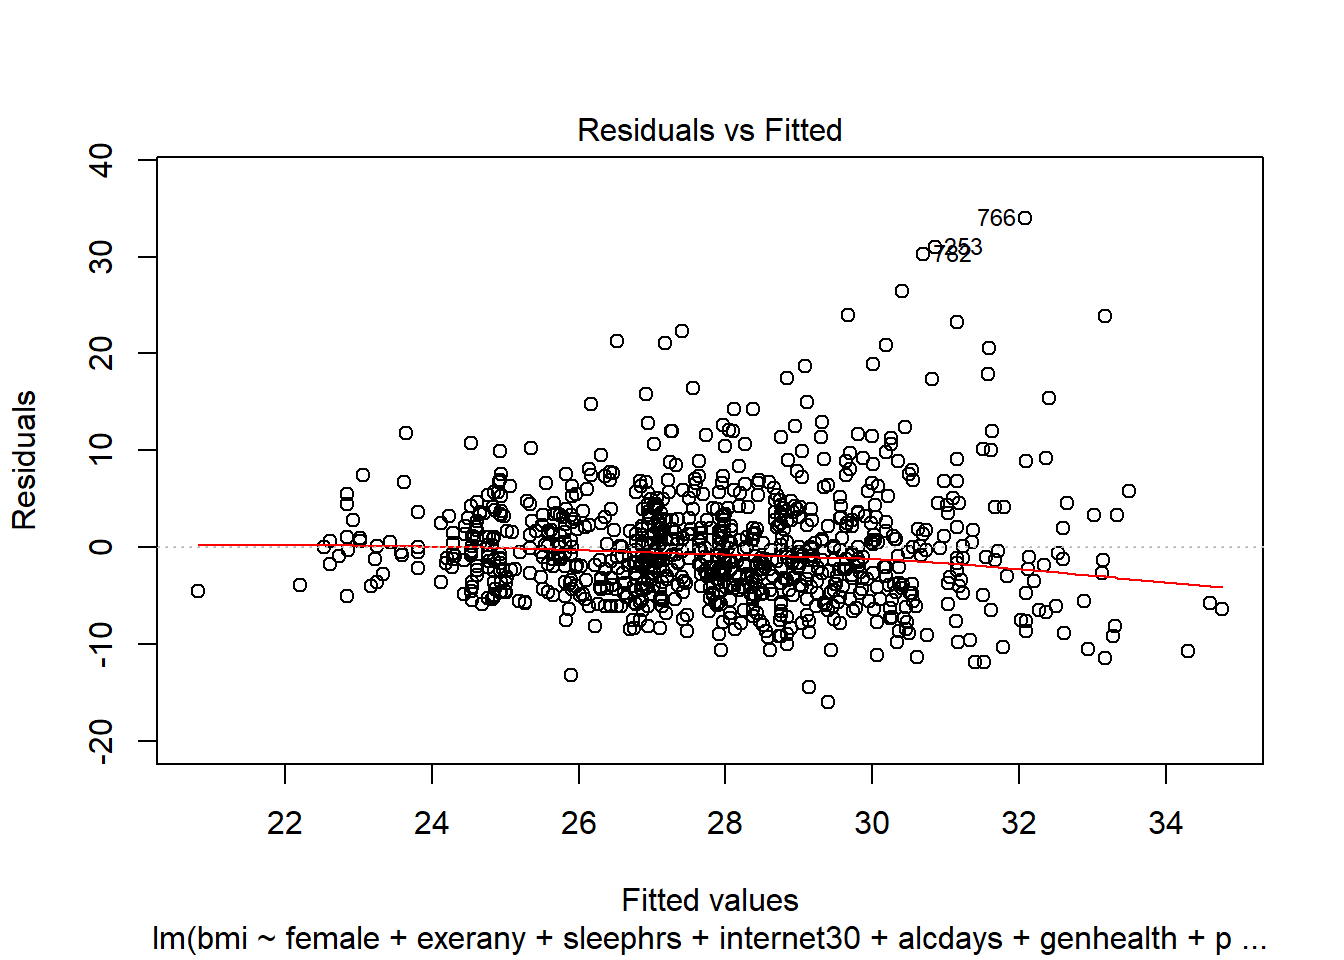
\includegraphics{bookdown-demo_files/figure-latex/residual_plot1_c2_m7-1.pdf}

\begin{enumerate}
\def\labelenumi{\arabic{enumi}.}
\setcounter{enumi}{1}
\tightlist
\item
  What can we conclude from the plot below?
\end{enumerate}

\begin{Shaded}
\begin{Highlighting}[]
\KeywordTok{plot}\NormalTok{(c2_m7, }\DataTypeTok{which =} \DecValTok{5}\NormalTok{)}
\end{Highlighting}
\end{Shaded}

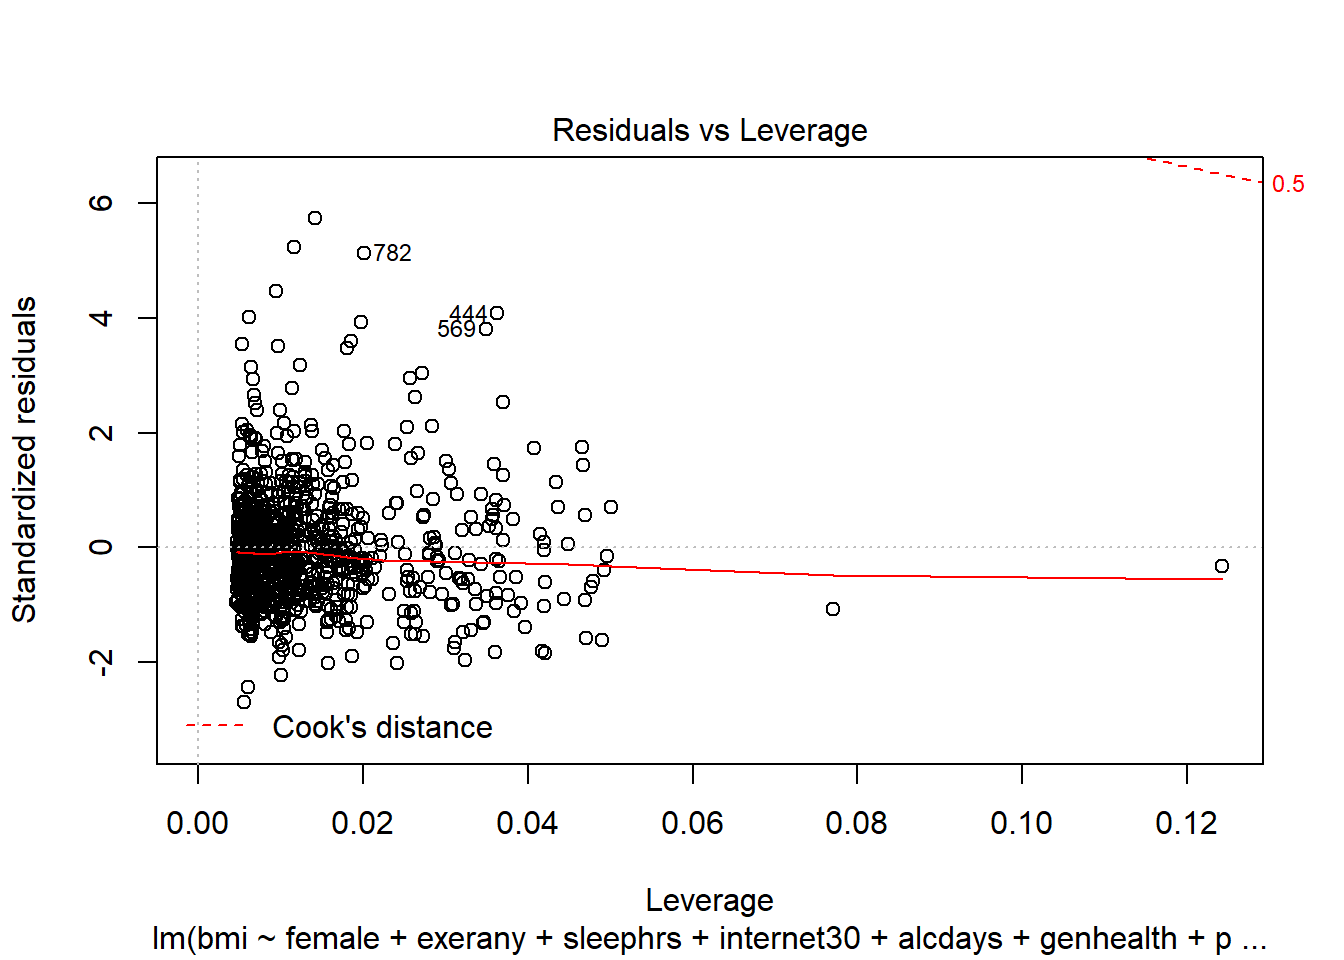
\includegraphics{bookdown-demo_files/figure-latex/residual_plot5_c2_m7-1.pdf}

\section{(DRAFT material) How might we validate this
model?}\label{draft-material-how-might-we-validate-this-model}

Here's some early code for that issue, which is built on some material
by David Robinson at \url{https://rpubs.com/dgrtwo/cv-modelr}

This bit of code performs what is called \emph{10-crossfold separation}.
In words, this approach splits the 896 observations in our data into 10
exclusive partitions of about 90\% into a training sample, and the
remaining 10\% in a test sample. The next part of the code maps a
modeling step to the training data, and then fits the resulting model on
the test data using the \texttt{broom} package's \texttt{augment}
function.

I've selected the variables in this case so that the model we'll fit is
the \texttt{m2\_c7} model we've been looking at, although there are
several ways to accomplish this.

\begin{Shaded}
\begin{Highlighting}[]
\KeywordTok{set.seed}\NormalTok{(}\DecValTok{4320118}\NormalTok{)}

\NormalTok{models <-}\StringTok{ }\NormalTok{smartcle2 }\OperatorTok
\StringTok{    }\KeywordTok{select}\NormalTok{(bmi, female, exerany, sleephrs, }
\NormalTok{           internet30, alcdays, genhealth) }\OperatorTok
\StringTok{    }\KeywordTok{crossv_kfold}\NormalTok{(}\DataTypeTok{k =} \DecValTok{10}\NormalTok{) }\OperatorTok
\StringTok{    }\KeywordTok{mutate}\NormalTok{(}\DataTypeTok{model =} \KeywordTok{map}\NormalTok{(train, }\OperatorTok{~}\StringTok{ }\KeywordTok{lm}\NormalTok{(bmi }\OperatorTok{~}\StringTok{ }\NormalTok{., }\DataTypeTok{data =}\NormalTok{ .)))}

\NormalTok{predictions <-}\StringTok{ }\NormalTok{models }\OperatorTok
\StringTok{    }\KeywordTok{unnest}\NormalTok{(}\KeywordTok{map2}\NormalTok{(model, test, }\OperatorTok{~}\StringTok{ }\KeywordTok{augment}\NormalTok{(.x, }\DataTypeTok{newdata =}\NormalTok{ .y)))}

\NormalTok{predictions}
\end{Highlighting}
\end{Shaded}

\begin{verbatim}
# A tibble: 896 x 10
   .id     bmi female exerany sleephrs internet30 alcdays genhealth  
   <chr> <dbl>  <int>   <int>    <int>      <int>   <int> <fct>      
 1 01     24.1      0       1        7          1       2 1_Excellent
 2 01     36.4      0       1        8          1       0 4_Fair     
 3 01     32.1      1       0        4          1       5 2_VeryGood 
 4 01     27.3      0       1        8          1       0 1_Excellent
 5 01     28.0      0       1        7          1       4 2_VeryGood 
 6 01     22.5      1       1        7          1       3 2_VeryGood 
 7 01     26.3      0       1        7          1       1 1_Excellent
 8 01     22.4      0       1        8          1       4 1_Excellent
 9 01     19.3      1       0        6          1       0 3_Good     
10 01     24.2      1       0        6          0       0 3_Good     
# ... with 886 more rows, and 2 more variables: .fitted <dbl>, .se.fit
#   <dbl>
\end{verbatim}

The results are a set of predictions based on the splits into training
and test groups (remember there are 10 of them, indexed by \texttt{.id})
that describe the complete set of 896 respondents again.

What this lets us now do is calculate the root Mean Squared Prediction
Error (RMSE) and Mean Absolute Prediction Error (MAE) for this model
(the \texttt{c2\_m7} model) across these observations, and also to
compare that error to a model that simply predicts the mean \texttt{bmi}
across all patients (the \texttt{intercept\ only} model.) In practice,
we could consider two distinct models in doing this work.

\begin{Shaded}
\begin{Highlighting}[]
\NormalTok{predictions }\OperatorTok
\StringTok{    }\KeywordTok{summarize}\NormalTok{(}\DataTypeTok{RMSE_c2_m7 =} \KeywordTok{sqrt}\NormalTok{(}\KeywordTok{mean}\NormalTok{((bmi }\OperatorTok{-}\StringTok{ }\NormalTok{.fitted) }\OperatorTok{^}\DecValTok{2}\NormalTok{)),}
              \DataTypeTok{MAE_c2_m7 =} \KeywordTok{mean}\NormalTok{(}\KeywordTok{abs}\NormalTok{(bmi }\OperatorTok{-}\StringTok{ }\NormalTok{.fitted)),}
              \DataTypeTok{RMSE_interceptonly =} \KeywordTok{sqrt}\NormalTok{(}\KeywordTok{mean}\NormalTok{((bmi }\OperatorTok{-}\StringTok{ }\KeywordTok{mean}\NormalTok{(bmi))}\OperatorTok{^}\DecValTok{2}\NormalTok{)),}
              \DataTypeTok{MAE_interceptonly =} \KeywordTok{mean}\NormalTok{(}\KeywordTok{abs}\NormalTok{(bmi }\OperatorTok{-}\StringTok{ }\KeywordTok{mean}\NormalTok{(bmi))))}
\end{Highlighting}
\end{Shaded}

\begin{verbatim}
# A tibble: 1 x 4
  RMSE_c2_m7 MAE_c2_m7 RMSE_interceptonly MAE_interceptonly
       <dbl>     <dbl>              <dbl>             <dbl>
1       6.03      4.40               6.32              4.59
\end{verbatim}

Another thing we could do with this tibble of predictions we have
created is to graph the size of the prediction errors (observed
\texttt{bmi} minus predicted values in \texttt{.fitted}) that our
modeling approach makes.

\begin{Shaded}
\begin{Highlighting}[]
\NormalTok{predictions }\OperatorTok
\StringTok{    }\KeywordTok{mutate}\NormalTok{(}\DataTypeTok{errors =}\NormalTok{ bmi }\OperatorTok{-}\StringTok{ }\NormalTok{.fitted) }\OperatorTok
\StringTok{    }\KeywordTok{ggplot}\NormalTok{(., }\KeywordTok{aes}\NormalTok{(}\DataTypeTok{x =}\NormalTok{ errors)) }\OperatorTok{+}
\StringTok{    }\KeywordTok{geom_histogram}\NormalTok{(}\DataTypeTok{bins =} \DecValTok{30}\NormalTok{, }\DataTypeTok{fill =} \StringTok{"darkviolet"}\NormalTok{, }\DataTypeTok{col =} \StringTok{"yellow"}\NormalTok{) }\OperatorTok{+}\StringTok{ }
\StringTok{    }\KeywordTok{labs}\NormalTok{(}\DataTypeTok{title =} \StringTok{"Cross-Validated Errors in Prediction of BMI"}\NormalTok{,}
         \DataTypeTok{subtitle =} \StringTok{"Using a model (`c2_m7`) including 6 regression inputs"}\NormalTok{,}
         \DataTypeTok{caption =} \StringTok{"SMART BRFSS 2016 data for Cleveland-Elyria MMSA, n = 896"}\NormalTok{,}
         \DataTypeTok{x =} \StringTok{"Error in predicting BMI"}\NormalTok{)}
\end{Highlighting}
\end{Shaded}

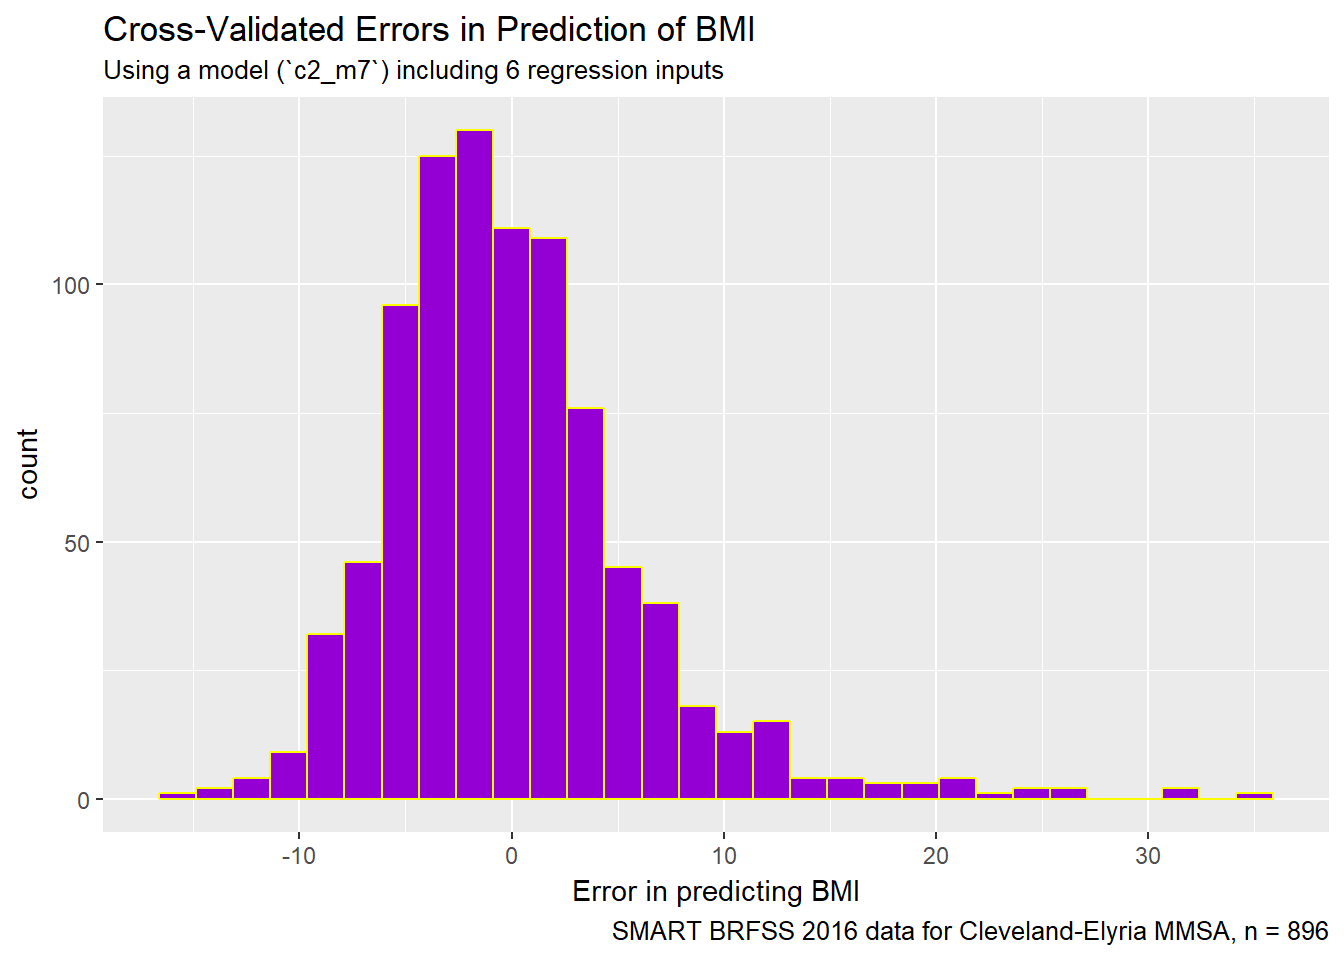
\includegraphics{bookdown-demo_files/figure-latex/validation_c2_m7_first_approach_errorhistogram-1.pdf}

\section{Coming Soon \ldots{}}\label{coming-soon}

\begin{enumerate}
\def\labelenumi{\arabic{enumi}.}
\tightlist
\item
  Would stepwise regression help us build a better model for
  \texttt{bmi}?

  \begin{itemize}
  \tightlist
  \item
    Is there a better approach for variable selection? What's this I
    hear about ``best subsets'', for example?
  \end{itemize}
\item
  How should we think about potential transformations of these
  predictors?

  \begin{itemize}
  \tightlist
  \item
    What's a Spearman rho-squared plot, and how might it help us decide
    how to spend degrees of freedom on non-linear terms better?
  \end{itemize}
\item
  How do we deal with missing data in fitting and evaluating a linear
  regression model if we don't actually want to drop all of the
  incomplete cases?
\item
  How can we use the \texttt{ols} tool in the \texttt{rms} package to
  fit regression models?
\item
  How can we use the tools in the \texttt{arm} package to fit and
  evaluate regression models?
\end{enumerate}

\chapter{Two-Factor Analysis of Variance and
Interactions}\label{two-factor-analysis-of-variance-and-interactions}

\section{\texorpdfstring{The \texttt{bonding} data: A Designed Dental
Experiment}{The bonding data: A Designed Dental Experiment}}\label{the-bonding-data-a-designed-dental-experiment}

The \texttt{bonding} data describe a designed experiment into the
properties of four different resin types (\texttt{resin} = A, B, C, D)
and two different curing light sources (\texttt{light} = Halogen, LED)
as they relate to the resulting bonding strength (measured in
MPa\footnote{The MPa is defined as the failure load (in Newtons) divided
  by the entire bonded area, in mm\textsuperscript{2}.}) on the surface
of teeth. The source is \citet{Kim2014}.

The experiment involved making measurements of bonding strength under a
total of 80 experimental setups, or runs, with 10 runs completed at each
of the eight combinations of a light source and a resin type. The data
are gathered in the \texttt{bonding.csv} file.

\begin{Shaded}
\begin{Highlighting}[]
\NormalTok{bonding}
\end{Highlighting}
\end{Shaded}

\begin{verbatim}
# A tibble: 80 x 4
   run_ID light   resin strength
   <fct>  <fct>   <fct>    <dbl>
 1 R101   LED     B         12.8
 2 R102   Halogen B         22.2
 3 R103   Halogen B         24.6
 4 R104   LED     A         17.0
 5 R105   LED     C         32.2
 6 R106   Halogen B         27.1
 7 R107   LED     A         23.4
 8 R108   Halogen A         23.5
 9 R109   Halogen D         37.3
10 R110   Halogen A         19.7
# ... with 70 more rows
\end{verbatim}

\subsection{Looking at the Data}\label{looking-at-the-data}

We can look at the distribution of the \texttt{strength} values at the
combinations of \texttt{light} and \texttt{resin}, with a plot like this
one\ldots{}

\begin{Shaded}
\begin{Highlighting}[]
\KeywordTok{ggplot}\NormalTok{(bonding, }\KeywordTok{aes}\NormalTok{(}\DataTypeTok{x =}\NormalTok{ resin, }\DataTypeTok{y =}\NormalTok{ strength, }\DataTypeTok{color =}\NormalTok{ light)) }\OperatorTok{+}
\StringTok{    }\KeywordTok{geom_point}\NormalTok{(}\DataTypeTok{size =} \DecValTok{2}\NormalTok{, }\DataTypeTok{alpha =} \FloatTok{0.5}\NormalTok{) }\OperatorTok{+}
\StringTok{    }\KeywordTok{facet_wrap}\NormalTok{(}\OperatorTok{~}\StringTok{ }\NormalTok{light) }\OperatorTok{+}
\StringTok{    }\KeywordTok{guides}\NormalTok{(}\DataTypeTok{color =} \OtherTok{FALSE}\NormalTok{) }\OperatorTok{+}
\StringTok{    }\KeywordTok{scale_color_manual}\NormalTok{(}\DataTypeTok{values =} \KeywordTok{c}\NormalTok{(}\StringTok{"purple"}\NormalTok{, }\StringTok{"darkorange"}\NormalTok{)) }\OperatorTok{+}
\StringTok{    }\KeywordTok{theme_bw}\NormalTok{() }
\end{Highlighting}
\end{Shaded}

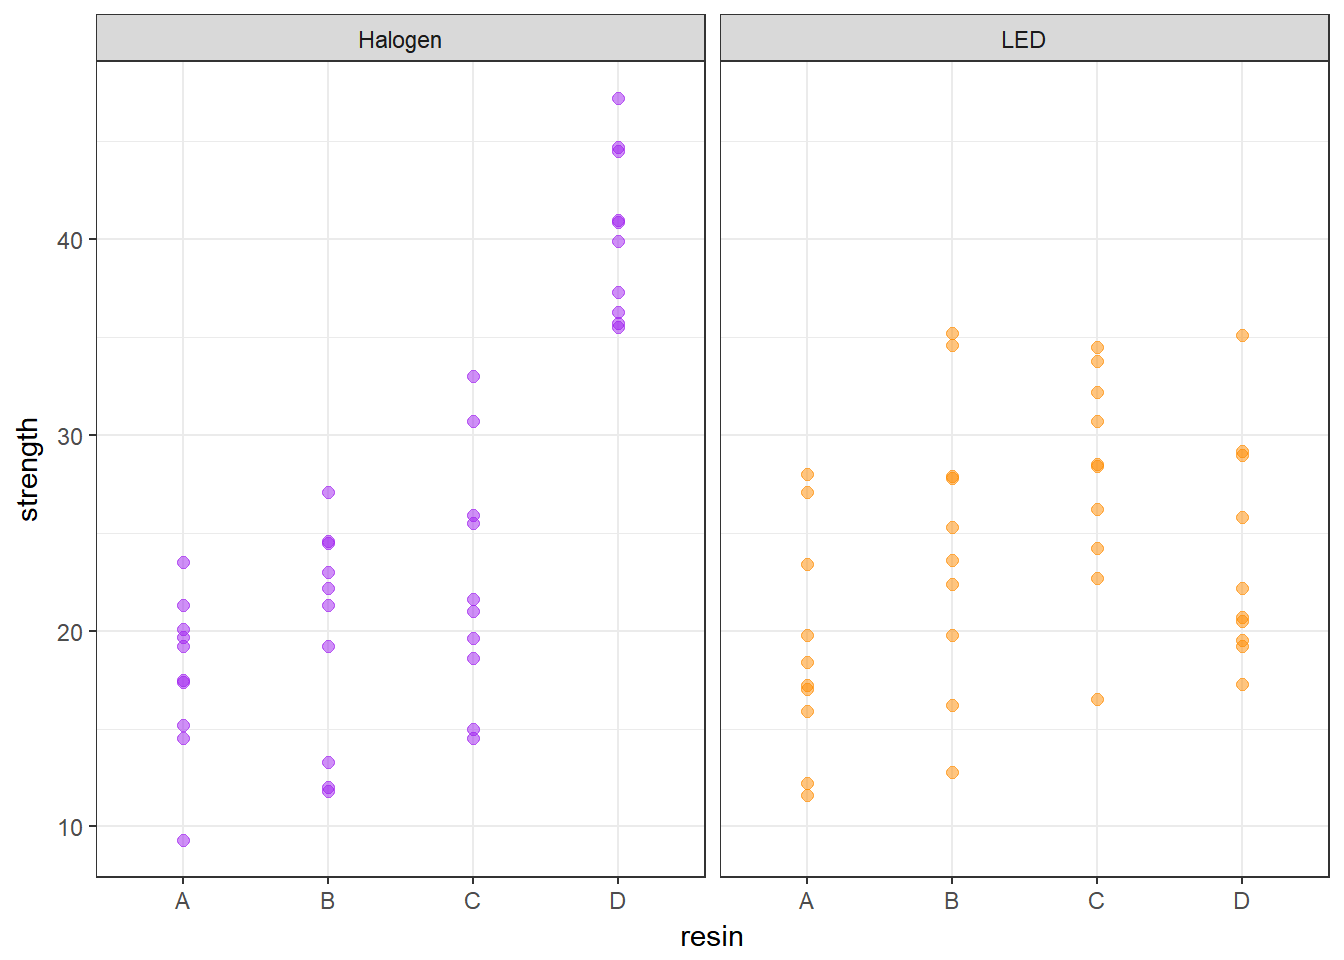
\includegraphics{bookdown-demo_files/figure-latex/c3_bonding_points_plot-1.pdf}

\section{A Means Plot (with standard deviations) to check for
interaction}\label{a-means-plot-with-standard-deviations-to-check-for-interaction}

Sometimes, we'll instead look at a plot simply of the means (and, often,
the standard deviations) of \texttt{strength} at each combination of
\texttt{light} and \texttt{resin}. We'll start by building up a data set
with the summaries we want to plot.

\begin{Shaded}
\begin{Highlighting}[]
\NormalTok{bond.sum <-}\StringTok{ }\NormalTok{bonding }\OperatorTok\StringTok{ }
\StringTok{    }\KeywordTok{group_by}\NormalTok{(resin, light) }\OperatorTok
\StringTok{    }\KeywordTok{summarize}\NormalTok{(}\DataTypeTok{mean.str =} \KeywordTok{mean}\NormalTok{(strength), }\DataTypeTok{sd.str =} \KeywordTok{sd}\NormalTok{(strength))}

\NormalTok{bond.sum}
\end{Highlighting}
\end{Shaded}

\begin{verbatim}
# A tibble: 8 x 4
# Groups: resin [?]
  resin light   mean.str sd.str
  <fct> <fct>      <dbl>  <dbl>
1 A     Halogen     17.8   4.02
2 A     LED         19.1   5.63
3 B     Halogen     19.9   5.62
4 B     LED         24.6   7.25
5 C     Halogen     22.5   6.19
6 C     LED         27.8   5.56
7 D     Halogen     40.3   4.15
8 D     LED         23.8   5.70
\end{verbatim}

Now, we'll use this new data set to plot the means and standard
deviations of \texttt{strength} at each combination of \texttt{resin}
and \texttt{light}.

\begin{Shaded}
\begin{Highlighting}[]
\NormalTok{## The error bars will overlap unless we adjust the position.}
\NormalTok{pd <-}\StringTok{ }\KeywordTok{position_dodge}\NormalTok{(}\FloatTok{0.2}\NormalTok{) }\CommentTok{# move them .1 to the left and right}

\KeywordTok{ggplot}\NormalTok{(bond.sum, }\KeywordTok{aes}\NormalTok{(}\DataTypeTok{x =}\NormalTok{ resin, }\DataTypeTok{y =}\NormalTok{ mean.str, }\DataTypeTok{col =}\NormalTok{ light)) }\OperatorTok{+}
\StringTok{    }\KeywordTok{geom_errorbar}\NormalTok{(}\KeywordTok{aes}\NormalTok{(}\DataTypeTok{ymin =}\NormalTok{ mean.str }\OperatorTok{-}\StringTok{ }\NormalTok{sd.str, }
                      \DataTypeTok{ymax =}\NormalTok{ mean.str }\OperatorTok{+}\StringTok{ }\NormalTok{sd.str),}
                  \DataTypeTok{width =} \FloatTok{0.2}\NormalTok{, }\DataTypeTok{position =}\NormalTok{ pd) }\OperatorTok{+}
\StringTok{    }\KeywordTok{geom_point}\NormalTok{(}\DataTypeTok{size =} \DecValTok{2}\NormalTok{, }\DataTypeTok{position =}\NormalTok{ pd) }\OperatorTok{+}\StringTok{ }
\StringTok{    }\KeywordTok{geom_line}\NormalTok{(}\KeywordTok{aes}\NormalTok{(}\DataTypeTok{group =}\NormalTok{ light), }\DataTypeTok{position =}\NormalTok{ pd) }\OperatorTok{+}
\StringTok{    }\KeywordTok{scale_color_manual}\NormalTok{(}\DataTypeTok{values =} \KeywordTok{c}\NormalTok{(}\StringTok{"purple"}\NormalTok{, }\StringTok{"darkorange"}\NormalTok{)) }\OperatorTok{+}
\StringTok{    }\KeywordTok{theme_bw}\NormalTok{() }\OperatorTok{+}
\StringTok{    }\KeywordTok{labs}\NormalTok{(}\DataTypeTok{y =} \StringTok{"Bonding Strength (MPa)"}\NormalTok{, }\DataTypeTok{x =} \StringTok{"Resin Type"}\NormalTok{,}
         \DataTypeTok{title =} \StringTok{"Observed Means (+/- SD) of Bonding Strength"}\NormalTok{)}
\end{Highlighting}
\end{Shaded}

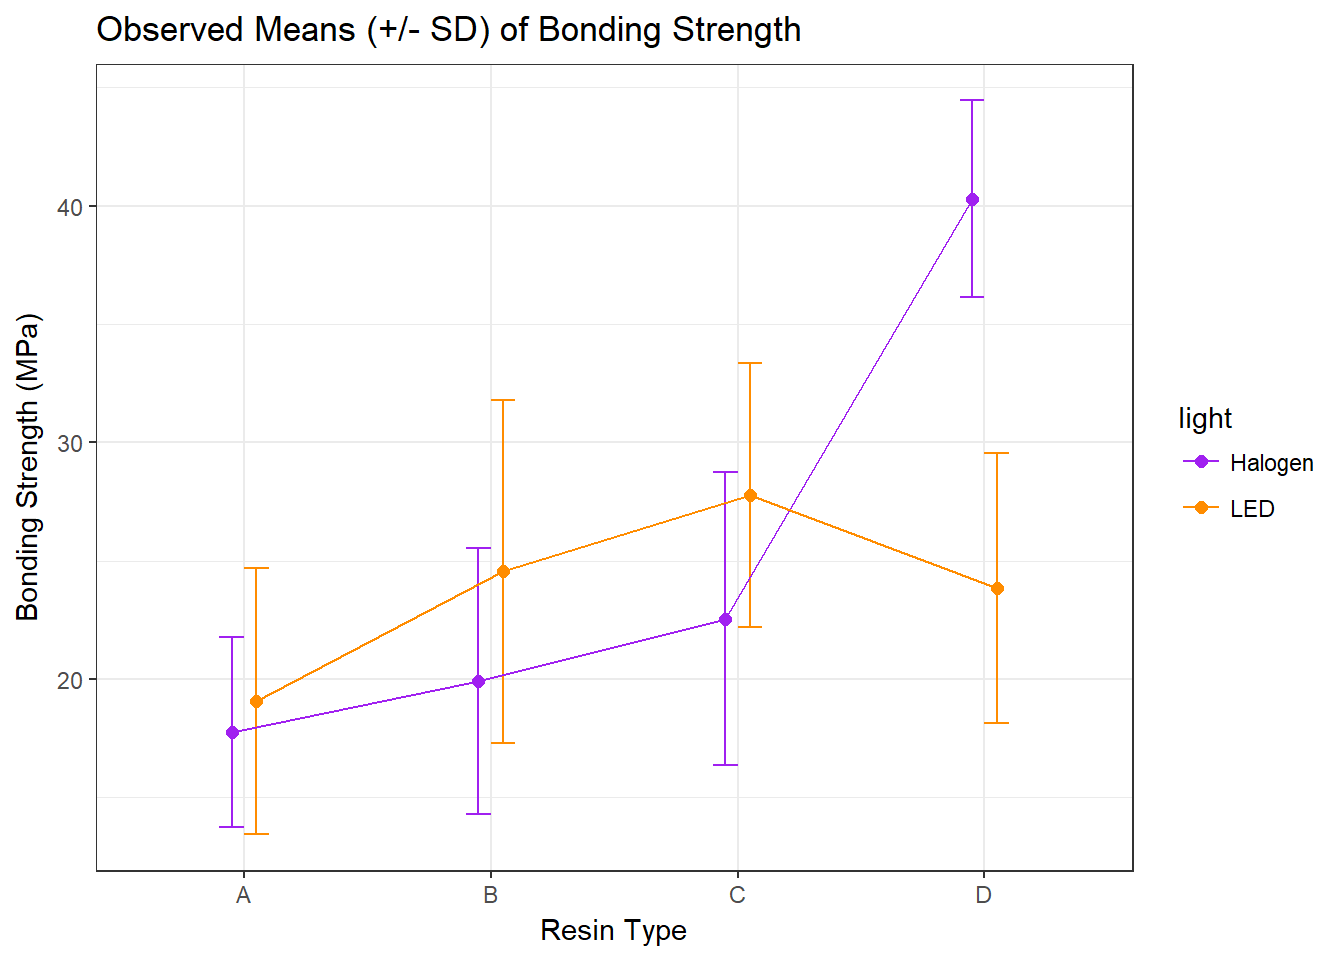
\includegraphics{bookdown-demo_files/figure-latex/c3_ggplot_means_plot_bonding-1.pdf}

Is there evidence of a meaningful interaction between the resin type and
the \texttt{light} source on the bonding strength in this plot?

\begin{itemize}
\tightlist
\item
  Sure. A meaningful interaction just means that the strength associated
  with different \texttt{resin} types depends on the \texttt{light}
  source.

  \begin{itemize}
  \tightlist
  \item
    With LED \texttt{light}, it appears that \texttt{resin} C leads to
    the strongest bonding strength.
  \item
    With Halogen \texttt{light}, though, it seems that \texttt{resin} D
    is substantially stronger.
  \end{itemize}
\item
  Note that the lines we see here connecting the \texttt{light} sources
  aren't in parallel (as they would be if we had zero interaction
  between \texttt{resin} and \texttt{light}), but rather, they cross.
\end{itemize}

\subsection{\texorpdfstring{Skimming the data after grouping by
\texttt{resin} and
\texttt{light}}{Skimming the data after grouping by resin and light}}\label{skimming-the-data-after-grouping-by-resin-and-light}

We might want to look at a numerical summary of the \texttt{strengths}
within these groups, too.

\begin{Shaded}
\begin{Highlighting}[]
\NormalTok{bonding }\OperatorTok
\StringTok{    }\KeywordTok{group_by}\NormalTok{(resin, light) }\OperatorTok
\StringTok{    }\KeywordTok{skim}\NormalTok{(strength) }
\end{Highlighting}
\end{Shaded}

\begin{verbatim}
Skim summary statistics
 n obs: 80 
 n variables: 4 
 group variables: resin, light 

Variable type: numeric 
 resin   light variable missing complete  n  mean   sd   p0   p25 median
     A Halogen strength       0       10 10 17.77 4.02  9.3 15.75  18.35
     A     LED strength       0       10 10 19.06 5.63 11.6 16.18  17.8 
     B Halogen strength       0       10 10 19.9  5.62 11.8 14.78  21.75
     B     LED strength       0       10 10 24.56 7.25 12.8 20.45  24.45
     C Halogen strength       0       10 10 22.54 6.19 14.5 18.85  21.3 
     C     LED strength       0       10 10 27.77 5.56 16.5 24.7   28.45
     D Halogen strength       0       10 10 40.3  4.15 35.5 36.55  40.4 
     D     LED strength       0       10 10 23.85 5.7  17.3 19.75  21.45
   p75 p100
 20    23.5
 22.5  28  
 24.12 27.1
 27.87 35.2
 25.8  33  
 31.83 34.5
 43.62 47.2
 28.2  35.1
\end{verbatim}

\section{Fitting the Two-Way ANOVA model with
Interaction}\label{fitting-the-two-way-anova-model-with-interaction}

\begin{Shaded}
\begin{Highlighting}[]
\NormalTok{c3_m1 <-}\StringTok{ }\KeywordTok{lm}\NormalTok{(strength }\OperatorTok{~}\StringTok{ }\NormalTok{resin }\OperatorTok{*}\StringTok{ }\NormalTok{light, }\DataTypeTok{data =}\NormalTok{ bonding)}

\KeywordTok{summary}\NormalTok{(c3_m1)}
\end{Highlighting}
\end{Shaded}

\begin{verbatim}

Call:
lm(formula = strength ~ resin * light, data = bonding)

Residuals:
    Min      1Q  Median      3Q     Max 
-11.760  -3.663  -0.320   3.697  11.250 

Coefficients:
                Estimate Std. Error t value Pr(>|t|)    
(Intercept)       17.770      1.771  10.033 2.57e-15 ***
resinB             2.130      2.505   0.850   0.3979    
resinC             4.770      2.505   1.904   0.0609 .  
resinD            22.530      2.505   8.995 2.13e-13 ***
lightLED           1.290      2.505   0.515   0.6081    
resinB:lightLED    3.370      3.542   0.951   0.3446    
resinC:lightLED    3.940      3.542   1.112   0.2697    
resinD:lightLED  -17.740      3.542  -5.008 3.78e-06 ***
---
Signif. codes:  0 '***' 0.001 '**' 0.01 '*' 0.05 '.' 0.1 ' ' 1

Residual standard error: 5.601 on 72 degrees of freedom
Multiple R-squared:  0.6149,    Adjusted R-squared:  0.5775 
F-statistic: 16.42 on 7 and 72 DF,  p-value: 9.801e-13
\end{verbatim}

\subsection{The ANOVA table for our
model}\label{the-anova-table-for-our-model}

In a two-way ANOVA model, we begin by assessing the interaction term. If
it's important, then our best model is the model including the
interaction. If it's not important, we will often move on to consider a
new model, fit without an interaction.

The ANOVA table is especially helpful in this case, because it lets us
look specifically at the interaction effect.

\begin{Shaded}
\begin{Highlighting}[]
\KeywordTok{anova}\NormalTok{(c3_m1)}
\end{Highlighting}
\end{Shaded}

\begin{verbatim}
Analysis of Variance Table

Response: strength
            Df  Sum Sq Mean Sq F value    Pr(>F)    
resin        3 1999.72  666.57 21.2499 5.792e-10 ***
light        1   34.72   34.72  1.1067    0.2963    
resin:light  3 1571.96  523.99 16.7043 2.457e-08 ***
Residuals   72 2258.52   31.37                      
---
Signif. codes:  0 '***' 0.001 '**' 0.01 '*' 0.05 '.' 0.1 ' ' 1
\end{verbatim}

\subsection{Is the interaction
important?}\label{is-the-interaction-important}

In this case, the interaction:

\begin{itemize}
\tightlist
\item
  is evident in the means plot, and
\item
  is highly statistically significant, and
\item
  accounts for a sizeable fraction (27\%) of the overall variation
\end{itemize}

\[ 
\eta^2_{interaction} = \frac{\mbox{SS(resin:light)}}{SS(Total)}
= \frac{1571.96}{1999.72 + 34.72 + 1571.96 + 2258.52} = 0.268
\]

If the interaction were \emph{either} large or significant we would be
inclined to keep it in the model. In this case, it's both, so there's no
real reason to remove it.

\subsection{Interpreting the
Interaction}\label{interpreting-the-interaction}

Recall the model equation, which is:

\begin{Shaded}
\begin{Highlighting}[]
\NormalTok{c3_m1}
\end{Highlighting}
\end{Shaded}

\begin{verbatim}

Call:
lm(formula = strength ~ resin * light, data = bonding)

Coefficients:
    (Intercept)           resinB           resinC           resinD  
          17.77             2.13             4.77            22.53  
       lightLED  resinB:lightLED  resinC:lightLED  resinD:lightLED  
           1.29             3.37             3.94           -17.74  
\end{verbatim}

so we have:

\[
strength = 17.77 + 2.13 resinB + 4.77 resinC + 22.53 resinD \\
+ 1.29 lightLED + 3.37 resinB*lightLED \\
+ 3.94 resinC*lightLED - 17.74 resinD*lightLED
\]

So, if \texttt{light} = Halogen, our equation is:

\[
strength = 17.77 + 2.13 resinB + 4.77 resinC + 22.53 resinD 
\]

And if \texttt{light} = LED, our equation is:

\[
strength = 19.06 + 5.50 resinB + 8.71 resinC + 4.79 resinD 
\]

Note that both the intercept and the slopes change as a result of the
interaction. The model yields a different prediction for every possible
combination of a \texttt{resin} type and a \texttt{light} source.

\section{\texorpdfstring{Comparing Individual Combinations of
\texttt{resin} and
\texttt{light}}{Comparing Individual Combinations of resin and light}}\label{comparing-individual-combinations-of-resin-and-light}

To make comparisons between individual combinations of a \texttt{resin}
type and a \texttt{light} source, using something like Tukey's HSD
approach for multiple comparisons, we first refit the model using the
\texttt{aov} structure, rather than \texttt{lm}.

\begin{Shaded}
\begin{Highlighting}[]
\NormalTok{c3m1_aov <-}\StringTok{ }\KeywordTok{aov}\NormalTok{(strength }\OperatorTok{~}\StringTok{ }\NormalTok{resin }\OperatorTok{*}\StringTok{ }\NormalTok{light, }\DataTypeTok{data =}\NormalTok{ bonding)}

\KeywordTok{summary}\NormalTok{(c3m1_aov)}
\end{Highlighting}
\end{Shaded}

\begin{verbatim}
            Df Sum Sq Mean Sq F value   Pr(>F)    
resin        3 1999.7   666.6  21.250 5.79e-10 ***
light        1   34.7    34.7   1.107    0.296    
resin:light  3 1572.0   524.0  16.704 2.46e-08 ***
Residuals   72 2258.5    31.4                     
---
Signif. codes:  0 '***' 0.001 '**' 0.01 '*' 0.05 '.' 0.1 ' ' 1
\end{verbatim}

And now, we can obtain Tukey HSD comparisons (which will maintain an
overall 95\% family-wise confidence level) across the \texttt{resin}
types, the \texttt{light} sources, and the combinations, with the
TukeyHSD command. This approach is only completely appropriate if these
comparisons are pre-planned, and if the design is balanced (as this is,
with the same sample size for each combination of a \texttt{light}
source and \texttt{resin} type.)

\begin{Shaded}
\begin{Highlighting}[]
\KeywordTok{TukeyHSD}\NormalTok{(c3m1_aov)}
\end{Highlighting}
\end{Shaded}

\begin{verbatim}
  Tukey multiple comparisons of means
    95% family-wise confidence level

Fit: aov(formula = strength ~ resin * light, data = bonding)

$resin
      diff       lwr       upr     p adj
B-A  3.815 -0.843129  8.473129 0.1461960
C-A  6.740  2.081871 11.398129 0.0016436
D-A 13.660  9.001871 18.318129 0.0000000
C-B  2.925 -1.733129  7.583129 0.3568373
D-B  9.845  5.186871 14.503129 0.0000026
D-C  6.920  2.261871 11.578129 0.0011731

$light
               diff       lwr      upr     p adj
LED-Halogen -1.3175 -3.814042 1.179042 0.2963128

$`resin:light`
                      diff          lwr        upr     p adj
B:Halogen-A:Halogen   2.13  -5.68928258   9.949283 0.9893515
C:Halogen-A:Halogen   4.77  -3.04928258  12.589283 0.5525230
D:Halogen-A:Halogen  22.53  14.71071742  30.349283 0.0000000
A:LED-A:Halogen       1.29  -6.52928258   9.109283 0.9995485
B:LED-A:Halogen       6.79  -1.02928258  14.609283 0.1361092
C:LED-A:Halogen      10.00   2.18071742  17.819283 0.0037074
D:LED-A:Halogen       6.08  -1.73928258  13.899283 0.2443200
C:Halogen-B:Halogen   2.64  -5.17928258  10.459283 0.9640100
D:Halogen-B:Halogen  20.40  12.58071742  28.219283 0.0000000
A:LED-B:Halogen      -0.84  -8.65928258   6.979283 0.9999747
B:LED-B:Halogen       4.66  -3.15928258  12.479283 0.5818695
C:LED-B:Halogen       7.87   0.05071742  15.689283 0.0473914
D:LED-B:Halogen       3.95  -3.86928258  11.769283 0.7621860
D:Halogen-C:Halogen  17.76   9.94071742  25.579283 0.0000000
A:LED-C:Halogen      -3.48 -11.29928258   4.339283 0.8591455
B:LED-C:Halogen       2.02  -5.79928258   9.839283 0.9922412
C:LED-C:Halogen       5.23  -2.58928258  13.049283 0.4323859
D:LED-C:Halogen       1.31  -6.50928258   9.129283 0.9995004
A:LED-D:Halogen     -21.24 -29.05928258 -13.420717 0.0000000
B:LED-D:Halogen     -15.74 -23.55928258  -7.920717 0.0000006
C:LED-D:Halogen     -12.53 -20.34928258  -4.710717 0.0001014
D:LED-D:Halogen     -16.45 -24.26928258  -8.630717 0.0000002
B:LED-A:LED           5.50  -2.31928258  13.319283 0.3665620
C:LED-A:LED           8.71   0.89071742  16.529283 0.0185285
D:LED-A:LED           4.79  -3.02928258  12.609283 0.5471915
C:LED-B:LED           3.21  -4.60928258  11.029283 0.9027236
D:LED-B:LED          -0.71  -8.52928258   7.109283 0.9999920
D:LED-C:LED          -3.92 -11.73928258   3.899283 0.7690762
\end{verbatim}

One conclusion from this is that the combination of D and Halogen is
significantly stronger than each of the other seven combinations.

\section{\texorpdfstring{The \texttt{bonding} model without
Interaction}{The bonding model without Interaction}}\label{the-bonding-model-without-interaction}

It seems incorrect in this situation to fit a model without the
interaction term, but we'll do so just so you can see what's involved.

\begin{Shaded}
\begin{Highlighting}[]
\NormalTok{c3_m2 <-}\StringTok{ }\KeywordTok{lm}\NormalTok{(strength }\OperatorTok{~}\StringTok{ }\NormalTok{resin }\OperatorTok{+}\StringTok{ }\NormalTok{light, }\DataTypeTok{data =}\NormalTok{ bonding)}

\KeywordTok{summary}\NormalTok{(c3_m2)}
\end{Highlighting}
\end{Shaded}

\begin{verbatim}

Call:
lm(formula = strength ~ resin + light, data = bonding)

Residuals:
     Min       1Q   Median       3Q      Max 
-14.1163  -4.9531   0.1187   4.4613  14.4663 

Coefficients:
            Estimate Std. Error t value Pr(>|t|)    
(Intercept)   19.074      1.787  10.676  < 2e-16 ***
resinB         3.815      2.260   1.688  0.09555 .  
resinC         6.740      2.260   2.982  0.00386 ** 
resinD        13.660      2.260   6.044 5.39e-08 ***
lightLED      -1.317      1.598  -0.824  0.41229    
---
Signif. codes:  0 '***' 0.001 '**' 0.01 '*' 0.05 '.' 0.1 ' ' 1

Residual standard error: 7.147 on 75 degrees of freedom
Multiple R-squared:  0.3469,    Adjusted R-squared:  0.312 
F-statistic: 9.958 on 4 and 75 DF,  p-value: 1.616e-06
\end{verbatim}

In the no-interaction model, if \texttt{light} = Halogen, our equation
is:

\[
strength = 19.07 + 3.82 resinB + 6.74 resinC + 13.66 resinD
\]

And if \texttt{light} = LED, our equation is:

\[
strength = 17.75 + 3.82 resinB + 6.74 resinC + 13.66 resinD
\]

So, in the no-interaction model, only the intercept changes.

\begin{Shaded}
\begin{Highlighting}[]
\KeywordTok{anova}\NormalTok{(c3_m2)}
\end{Highlighting}
\end{Shaded}

\begin{verbatim}
Analysis of Variance Table

Response: strength
          Df Sum Sq Mean Sq F value    Pr(>F)    
resin      3 1999.7  666.57 13.0514 6.036e-07 ***
light      1   34.7   34.72  0.6797    0.4123    
Residuals 75 3830.5   51.07                      
---
Signif. codes:  0 '***' 0.001 '**' 0.01 '*' 0.05 '.' 0.1 ' ' 1
\end{verbatim}

And, it appears, if we ignore the interaction, then \texttt{resin} type
has a significant impact on \texttt{strength} but \texttt{light} source
doesn't. This is a bit clearer, when we look at boxplots of the
separated \texttt{light} and \texttt{resin} groups.

\begin{Shaded}
\begin{Highlighting}[]
\NormalTok{p1 <-}\StringTok{ }\KeywordTok{ggplot}\NormalTok{(bonding, }\KeywordTok{aes}\NormalTok{(}\DataTypeTok{x =}\NormalTok{ light, }\DataTypeTok{y =}\NormalTok{ strength)) }\OperatorTok{+}\StringTok{ }
\StringTok{    }\KeywordTok{geom_boxplot}\NormalTok{()}
\NormalTok{p2 <-}\StringTok{ }\KeywordTok{ggplot}\NormalTok{(bonding, }\KeywordTok{aes}\NormalTok{(}\DataTypeTok{x =}\NormalTok{ resin, }\DataTypeTok{y =}\NormalTok{ strength)) }\OperatorTok{+}
\StringTok{    }\KeywordTok{geom_boxplot}\NormalTok{()}

\NormalTok{gridExtra}\OperatorTok{::}\KeywordTok{grid.arrange}\NormalTok{(p1, p2, }\DataTypeTok{nrow =} \DecValTok{1}\NormalTok{)}
\end{Highlighting}
\end{Shaded}

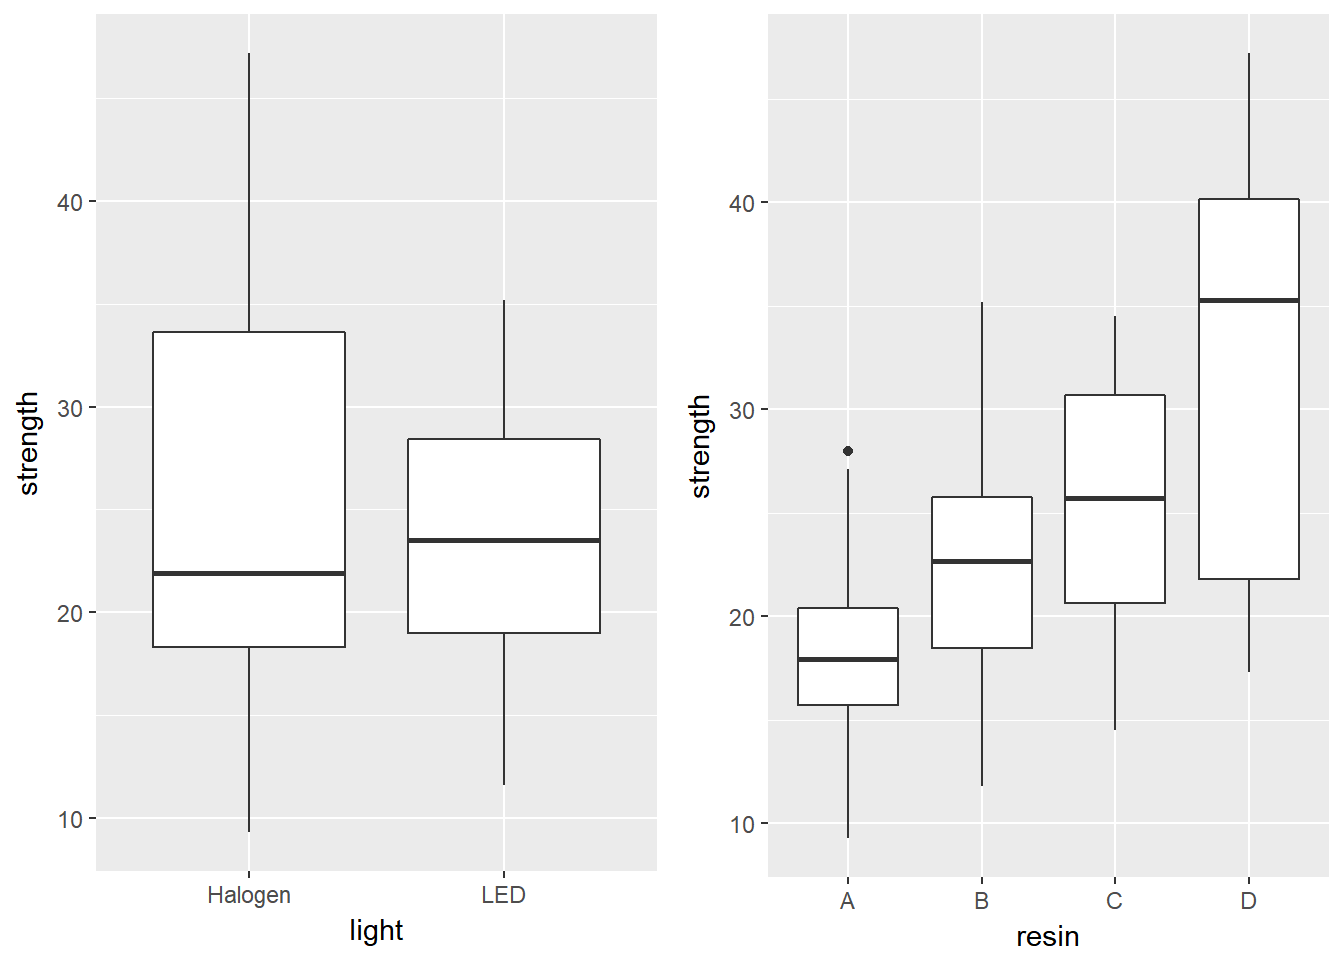
\includegraphics{bookdown-demo_files/figure-latex/boxplots_c3_bonding_without_interaction-1.pdf}

\section{\texorpdfstring{\texttt{cortisol}: A Hypothetical Clinical
Trial}{cortisol: A Hypothetical Clinical Trial}}\label{cortisol-a-hypothetical-clinical-trial}

156 adults who complained of problems with a high-stress lifestyle were
enrolled in a hypothetical clinical trial of the effectiveness of a
behavioral intervention designed to help reduce stress levels, as
measured by salivary cortisol.

The subjects were randomly assigned to one of three intervention groups
(usual care, low dose, and high dose.) The ``low dose'' subjects
received a one-week intervention with a follow-up at week 5. The ``high
dose'' subjects received a more intensive three-week intervention, with
follow up at week 5.

Since cortisol levels rise and fall with circadian rhythms, the cortisol
measurements were taken just after rising for all subjects. These
measurements were taken at baseline, and again at five weeks. The
difference (baseline - week 5) in cortisol level (in micrograms / l)
serves as the primary outcome.

\subsection{\texorpdfstring{Codebook and Raw Data for
\texttt{cortisol}}{Codebook and Raw Data for cortisol}}\label{codebook-and-raw-data-for-cortisol}

The data are gathered in the \texttt{cortisol} data set. Included are:

\begin{longtable}[]{@{}rl@{}}
\toprule
Variable & Description\tabularnewline
\midrule
\endhead
\texttt{subject} & subject identification code\tabularnewline
\texttt{interv} & intervention group (UC = usual care, Low,
High)\tabularnewline
\texttt{waist} & waist circumference at baseline (in
inches)\tabularnewline
\texttt{sex} & male or female\tabularnewline
\texttt{cort.1} & salivary cortisol level (microg/l) week
1\tabularnewline
\texttt{cort.5} & salivary cortisol level (microg/l) week
5\tabularnewline
\bottomrule
\end{longtable}

\begin{Shaded}
\begin{Highlighting}[]
\NormalTok{cortisol}
\end{Highlighting}
\end{Shaded}

\begin{verbatim}
# A tibble: 156 x 6
   subject interv waist sex   cort.1 cort.5
     <int> <fct>  <dbl> <fct>  <dbl>  <dbl>
 1    1001 UC      48.3 M      13.4   13.3 
 2    1002 Low     58.3 M      17.8   16.6 
 3    1003 High    43.0 M      14.4   12.7 
 4    1004 Low     44.9 M       9.00   9.80
 5    1005 High    46.1 M      14.2   14.2 
 6    1006 UC      41.3 M      14.8   15.1 
 7    1007 Low     51.0 F      13.7   16.0 
 8    1008 UC      42.0 F      17.3   18.7 
 9    1009 Low     24.7 F      15.3   15.8 
10    1010 Low     59.4 M      12.4   11.7 
# ... with 146 more rows
\end{verbatim}

\subsection{Creating a factor combining sex and
waist}\label{creating-a-factor-combining-sex-and-waist}

Next, we'll put the \texttt{waist} and \texttt{sex} data in the
\texttt{cortisol} example together. We want to build a second
categorical variable (called \texttt{fat\_est}) combining this
information, to indicate ``healthy'' vs. ``unhealthy'' levels of fat
around the waist.

\begin{itemize}
\tightlist
\item
  Male subjects whose waist circumference is 40 inches or more, and
\item
  Female subjects whose waist circumference is 35 inches or more, will
  fall in the ``unhealthy'' group.
\end{itemize}

\begin{Shaded}
\begin{Highlighting}[]
\NormalTok{cortisol <-}\StringTok{ }\NormalTok{cortisol }\OperatorTok
\StringTok{    }\KeywordTok{mutate}\NormalTok{(}
        \DataTypeTok{fat_est =} \KeywordTok{factor}\NormalTok{(}\KeywordTok{case_when}\NormalTok{(}
\NormalTok{            sex }\OperatorTok{==}\StringTok{ "M"} \OperatorTok{&}\StringTok{ }\NormalTok{waist }\OperatorTok{>=}\StringTok{ }\DecValTok{40} \OperatorTok{~}\StringTok{ "unhealthy"}\NormalTok{,}
\NormalTok{            sex }\OperatorTok{==}\StringTok{ "F"} \OperatorTok{&}\StringTok{ }\NormalTok{waist }\OperatorTok{>=}\StringTok{ }\DecValTok{35} \OperatorTok{~}\StringTok{ "unhealthy"}\NormalTok{,}
            \OtherTok{TRUE}                     \OperatorTok{~}\StringTok{ "healthy"}\NormalTok{)),}
        \DataTypeTok{cort_diff =}\NormalTok{ cort.}\DecValTok{1} \OperatorTok{-}\StringTok{ }\NormalTok{cort.}\DecValTok{5}\NormalTok{)}

\KeywordTok{summary}\NormalTok{(cortisol)}
\end{Highlighting}
\end{Shaded}

\begin{verbatim}
    subject      interv       waist       sex        cort.1      
 Min.   :1001   High:53   Min.   :20.80   F:83   Min.   : 6.000  
 1st Qu.:1040   Low :52   1st Qu.:33.27   M:73   1st Qu.: 9.675  
 Median :1078   UC  :51   Median :40.35          Median :12.400  
 Mean   :1078             Mean   :40.42          Mean   :12.686  
 3rd Qu.:1117             3rd Qu.:47.77          3rd Qu.:16.025  
 Max.   :1156             Max.   :59.90          Max.   :19.000  
     cort.5          fat_est      cort_diff      
 Min.   : 4.2   healthy  : 56   Min.   :-2.3000  
 1st Qu.: 9.6   unhealthy:100   1st Qu.:-0.5000  
 Median :12.6                   Median : 0.2000  
 Mean   :12.4                   Mean   : 0.2821  
 3rd Qu.:15.7                   3rd Qu.: 1.2000  
 Max.   :19.7                   Max.   : 2.0000  
\end{verbatim}

\section{\texorpdfstring{A Means Plot for the \texttt{cortisol} trial
(with standard
errors)}{A Means Plot for the cortisol trial (with standard errors)}}\label{a-means-plot-for-the-cortisol-trial-with-standard-errors}

Again, we'll start by building up a data set with the summaries we want
to plot.

\begin{Shaded}
\begin{Highlighting}[]
\NormalTok{cort.sum <-}\StringTok{ }\NormalTok{cortisol }\OperatorTok\StringTok{ }
\StringTok{    }\KeywordTok{group_by}\NormalTok{(interv, fat_est) }\OperatorTok
\StringTok{    }\KeywordTok{summarize}\NormalTok{(}\DataTypeTok{mean.cort =} \KeywordTok{mean}\NormalTok{(cort_diff), }
              \DataTypeTok{se.cort =} \KeywordTok{sd}\NormalTok{(cort_diff)}\OperatorTok{/}\KeywordTok{sqrt}\NormalTok{(}\KeywordTok{n}\NormalTok{()))}

\NormalTok{cort.sum}
\end{Highlighting}
\end{Shaded}

\begin{verbatim}
# A tibble: 6 x 4
# Groups: interv [?]
  interv fat_est   mean.cort se.cort
  <fct>  <fct>         <dbl>   <dbl>
1 High   healthy       0.695   0.217
2 High   unhealthy     0.352   0.150
3 Low    healthy       0.500   0.182
4 Low    unhealthy     0.327   0.190
5 UC     healthy       0.347   0.225
6 UC     unhealthy    -0.226   0.155
\end{verbatim}

Now, we'll use this new data set to plot the means and standard errors.

\begin{Shaded}
\begin{Highlighting}[]
\NormalTok{## The error bars will overlap unless we adjust the position.}
\NormalTok{pd <-}\StringTok{ }\KeywordTok{position_dodge}\NormalTok{(}\FloatTok{0.2}\NormalTok{) }\CommentTok{# move them .1 to the left and right}

\KeywordTok{ggplot}\NormalTok{(cort.sum, }\KeywordTok{aes}\NormalTok{(}\DataTypeTok{x =}\NormalTok{ interv, }\DataTypeTok{y =}\NormalTok{ mean.cort, }\DataTypeTok{col =}\NormalTok{ fat_est)) }\OperatorTok{+}
\StringTok{    }\KeywordTok{geom_errorbar}\NormalTok{(}\KeywordTok{aes}\NormalTok{(}\DataTypeTok{ymin =}\NormalTok{ mean.cort }\OperatorTok{-}\StringTok{ }\NormalTok{se.cort, }
                      \DataTypeTok{ymax =}\NormalTok{ mean.cort }\OperatorTok{+}\StringTok{ }\NormalTok{se.cort),}
                  \DataTypeTok{width =} \FloatTok{0.2}\NormalTok{, }\DataTypeTok{position =}\NormalTok{ pd) }\OperatorTok{+}
\StringTok{    }\KeywordTok{geom_point}\NormalTok{(}\DataTypeTok{size =} \DecValTok{2}\NormalTok{, }\DataTypeTok{position =}\NormalTok{ pd) }\OperatorTok{+}\StringTok{ }
\StringTok{    }\KeywordTok{geom_line}\NormalTok{(}\KeywordTok{aes}\NormalTok{(}\DataTypeTok{group =}\NormalTok{ fat_est), }\DataTypeTok{position =}\NormalTok{ pd) }\OperatorTok{+}
\StringTok{    }\KeywordTok{scale_color_manual}\NormalTok{(}\DataTypeTok{values =} \KeywordTok{c}\NormalTok{(}\StringTok{"royalblue"}\NormalTok{, }\StringTok{"darkred"}\NormalTok{)) }\OperatorTok{+}
\StringTok{    }\KeywordTok{theme_bw}\NormalTok{() }\OperatorTok{+}
\StringTok{    }\KeywordTok{labs}\NormalTok{(}\DataTypeTok{y =} \StringTok{"Salivary Cortisol Level"}\NormalTok{, }\DataTypeTok{x =} \StringTok{"Intervention Group"}\NormalTok{,}
         \DataTypeTok{title =} \StringTok{"Observed Means (+/- SE) of Salivary Cortisol"}\NormalTok{)}
\end{Highlighting}
\end{Shaded}

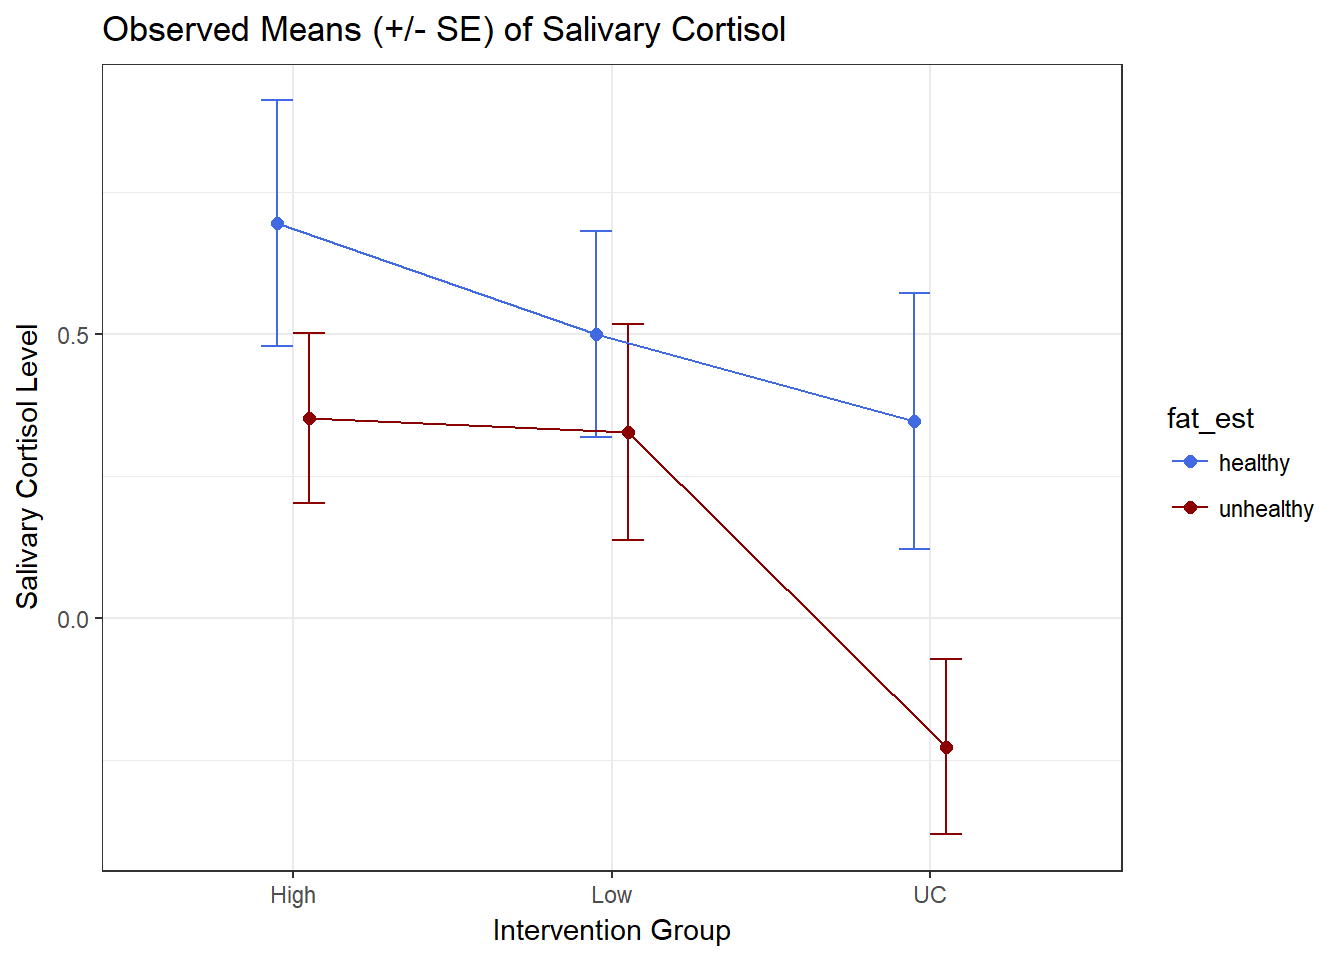
\includegraphics{bookdown-demo_files/figure-latex/c3_ggplot_means_plot_cortisol-1.pdf}

\section{\texorpdfstring{A Two-Way ANOVA model for \texttt{cortisol}
with
Interaction}{A Two-Way ANOVA model for cortisol with Interaction}}\label{a-two-way-anova-model-for-cortisol-with-interaction}

\begin{Shaded}
\begin{Highlighting}[]
\NormalTok{c3_m3 <-}\StringTok{ }\KeywordTok{lm}\NormalTok{(cort_diff }\OperatorTok{~}\StringTok{ }\NormalTok{interv }\OperatorTok{*}\StringTok{ }\NormalTok{fat_est, }\DataTypeTok{data =}\NormalTok{ cortisol)}

\KeywordTok{anova}\NormalTok{(c3_m3)}
\end{Highlighting}
\end{Shaded}

\begin{verbatim}
Analysis of Variance Table

Response: cort_diff
                Df  Sum Sq Mean Sq F value  Pr(>F)  
interv           2   7.847  3.9235  4.4698 0.01301 *
fat_est          1   4.614  4.6139  5.2564 0.02326 *
interv:fat_est   2   0.943  0.4715  0.5371 0.58554  
Residuals      150 131.666  0.8778                  
---
Signif. codes:  0 '***' 0.001 '**' 0.01 '*' 0.05 '.' 0.1 ' ' 1
\end{verbatim}

Does it seem like we need the interaction term in this case?

\begin{Shaded}
\begin{Highlighting}[]
\KeywordTok{summary}\NormalTok{(c3_m3)}
\end{Highlighting}
\end{Shaded}

\begin{verbatim}

Call:
lm(formula = cort_diff ~ interv * fat_est, data = cortisol)

Residuals:
     Min       1Q   Median       3Q      Max 
-2.62727 -0.75702  0.08636  0.84848  2.12647 

Coefficients:
                           Estimate Std. Error t value Pr(>|t|)   
(Intercept)                  0.6950     0.2095   3.317  0.00114 **
intervLow                   -0.1950     0.3001  -0.650  0.51689   
intervUC                    -0.3479     0.3091  -1.126  0.26206   
fat_estunhealthy            -0.3435     0.2655  -1.294  0.19774   
intervLow:fat_estunhealthy   0.1708     0.3785   0.451  0.65256   
intervUC:fat_estunhealthy   -0.2300     0.3846  -0.598  0.55068   
---
Signif. codes:  0 '***' 0.001 '**' 0.01 '*' 0.05 '.' 0.1 ' ' 1

Residual standard error: 0.9369 on 150 degrees of freedom
Multiple R-squared:  0.0924,    Adjusted R-squared:  0.06214 
F-statistic: 3.054 on 5 and 150 DF,  p-value: 0.01179
\end{verbatim}

How do you reconcile the apparent difference in significance levels
between this regression summary and the ANOVA table above?

\section{\texorpdfstring{A Two-Way ANOVA model for \texttt{cortisol}
without
Interaction}{A Two-Way ANOVA model for cortisol without Interaction}}\label{a-two-way-anova-model-for-cortisol-without-interaction}

\subsection{The Graph}\label{the-graph}

\begin{Shaded}
\begin{Highlighting}[]
\NormalTok{p1 <-}\StringTok{ }\KeywordTok{ggplot}\NormalTok{(cortisol, }\KeywordTok{aes}\NormalTok{(}\DataTypeTok{x =}\NormalTok{ interv, }\DataTypeTok{y =}\NormalTok{ cort_diff)) }\OperatorTok{+}\StringTok{ }
\StringTok{    }\KeywordTok{geom_boxplot}\NormalTok{()}
\NormalTok{p2 <-}\StringTok{ }\KeywordTok{ggplot}\NormalTok{(cortisol, }\KeywordTok{aes}\NormalTok{(}\DataTypeTok{x =}\NormalTok{ fat_est, }\DataTypeTok{y =}\NormalTok{ cort_diff)) }\OperatorTok{+}
\StringTok{    }\KeywordTok{geom_boxplot}\NormalTok{()}

\NormalTok{gridExtra}\OperatorTok{::}\KeywordTok{grid.arrange}\NormalTok{(p1, p2, }\DataTypeTok{nrow =} \DecValTok{1}\NormalTok{)}
\end{Highlighting}
\end{Shaded}

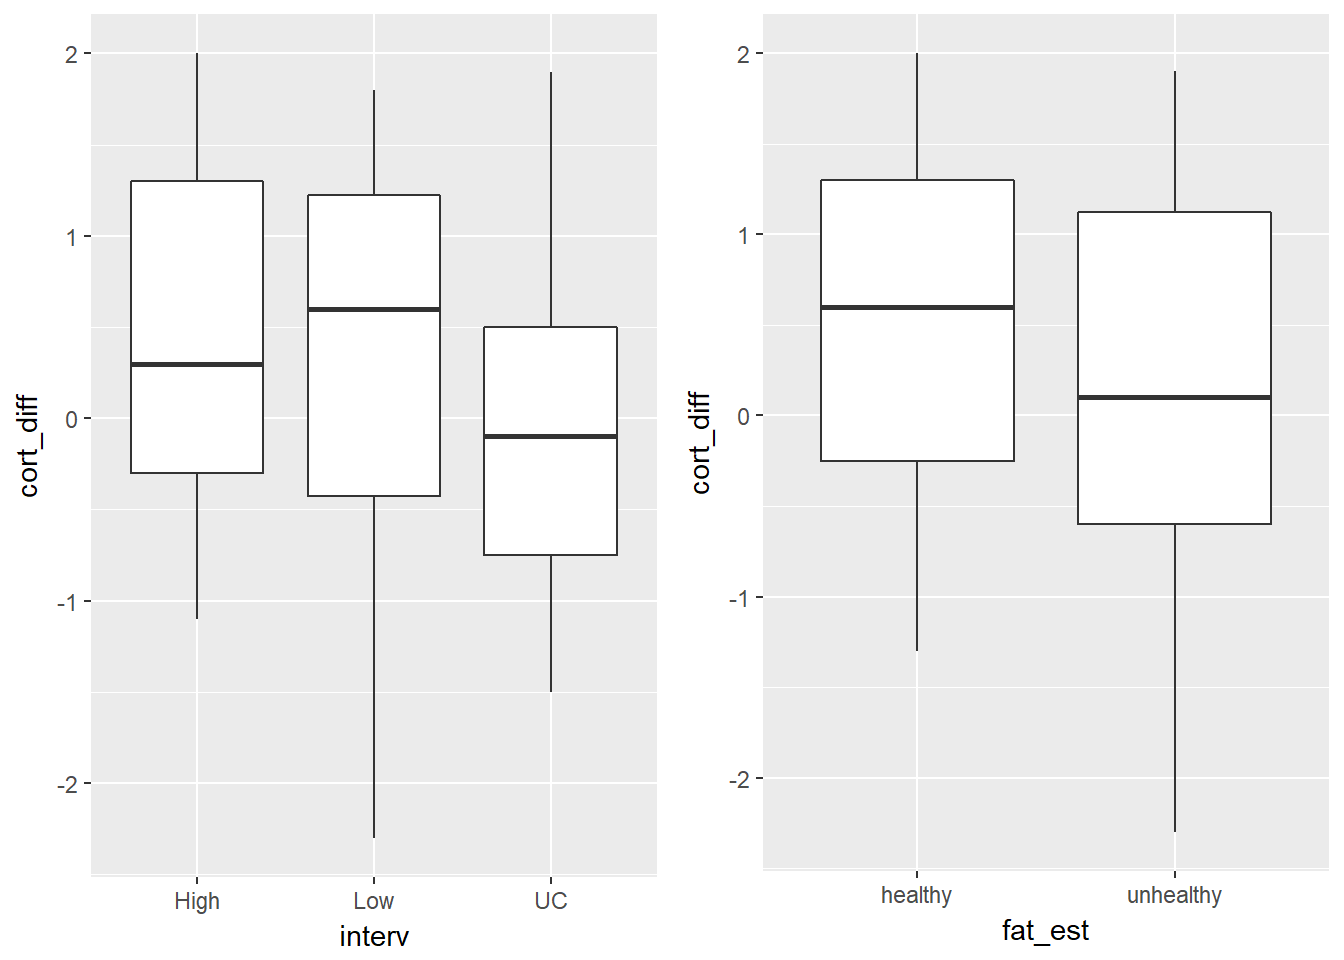
\includegraphics{bookdown-demo_files/figure-latex/boxplots_c3_cortisol_without_interaction-1.pdf}

\subsection{The ANOVA Model}\label{the-anova-model}

\begin{Shaded}
\begin{Highlighting}[]
\NormalTok{c3_m4 <-}\StringTok{ }\KeywordTok{lm}\NormalTok{(cort_diff }\OperatorTok{~}\StringTok{ }\NormalTok{interv }\OperatorTok{+}\StringTok{ }\NormalTok{fat_est, }\DataTypeTok{data =}\NormalTok{ cortisol)}

\KeywordTok{anova}\NormalTok{(c3_m4)}
\end{Highlighting}
\end{Shaded}

\begin{verbatim}
Analysis of Variance Table

Response: cort_diff
           Df  Sum Sq Mean Sq F value  Pr(>F)  
interv      2   7.847  3.9235  4.4972 0.01266 *
fat_est     1   4.614  4.6139  5.2886 0.02283 *
Residuals 152 132.609  0.8724                  
---
Signif. codes:  0 '***' 0.001 '**' 0.01 '*' 0.05 '.' 0.1 ' ' 1
\end{verbatim}

How do these results compare to those we saw in the model with
interaction?

\subsection{The Regression Summary}\label{the-regression-summary}

\begin{Shaded}
\begin{Highlighting}[]
\KeywordTok{summary}\NormalTok{(c3_m4)}
\end{Highlighting}
\end{Shaded}

\begin{verbatim}

Call:
lm(formula = cort_diff ~ interv + fat_est, data = cortisol)

Residuals:
     Min       1Q   Median       3Q      Max 
-2.55929 -0.74527  0.05457  0.86456  2.05489 

Coefficients:
                 Estimate Std. Error t value Pr(>|t|)    
(Intercept)       0.70452    0.16093   4.378 2.22e-05 ***
intervLow        -0.08645    0.18232  -0.474  0.63606    
intervUC         -0.50063    0.18334  -2.731  0.00707 ** 
fat_estunhealthy -0.35878    0.15601  -2.300  0.02283 *  
---
Signif. codes:  0 '***' 0.001 '**' 0.01 '*' 0.05 '.' 0.1 ' ' 1

Residual standard error: 0.934 on 152 degrees of freedom
Multiple R-squared:  0.0859,    Adjusted R-squared:  0.06785 
F-statistic: 4.761 on 3 and 152 DF,  p-value: 0.00335
\end{verbatim}

\subsection{Tukey HSD Comparisons}\label{tukey-hsd-comparisons}

Without the interaction term, we can make direct comparisons between
levels of the intervention, and between levels of the \texttt{fat\_est}
variable. This is probably best done here in a Tukey HSD comparison.

\begin{Shaded}
\begin{Highlighting}[]
\KeywordTok{TukeyHSD}\NormalTok{(}\KeywordTok{aov}\NormalTok{(cort_diff }\OperatorTok{~}\StringTok{ }\NormalTok{interv }\OperatorTok{+}\StringTok{ }\NormalTok{fat_est, }\DataTypeTok{data =}\NormalTok{ cortisol))}
\end{Highlighting}
\end{Shaded}

\begin{verbatim}
  Tukey multiple comparisons of means
    95% family-wise confidence level

Fit: aov(formula = cort_diff ~ interv + fat_est, data = cortisol)

$interv
                diff        lwr         upr     p adj
Low-High -0.09074746 -0.5222655  0.34077063 0.8724916
UC-High  -0.51642619 -0.9500745 -0.08277793 0.0150150
UC-Low   -0.42567873 -0.8613670  0.01000948 0.0570728

$fat_est
                        diff        lwr         upr     p adj
unhealthy-healthy -0.3582443 -0.6662455 -0.05024305 0.0229266
\end{verbatim}

What conclusions can we draw, at a 5\% significance level?

\chapter{Missing Data, 1: Mechanisms and Single Imputation
Methods}\label{missing-data-1-mechanisms-and-single-imputation-methods}

Almost all serious statistical analyses have to deal with missing data.
Data values that are missing are indicated in R, and to R, by the symbol
\texttt{NA}.

\section{A Toy Example}\label{a-toy-example}

In the following tiny data set called \texttt{sbp\_example}, we have
four variables for a set of 15 subjects. In addition to a subject id, we
have:

\begin{itemize}
\tightlist
\item
  the treatment this subject received (A, B or C are the treatments),
\item
  an indicator (1 = yes, 0 = no) of whether the subject has diabetes,
\item
  the subject's systolic blood pressure at baseline
\item
  the subject's systolic blood pressure after the application of the
  treatment
\end{itemize}

\begin{Shaded}
\begin{Highlighting}[]
\CommentTok{# create some temporary variables}

\NormalTok{subject <-}\StringTok{ }\DecValTok{101}\OperatorTok{:}\DecValTok{115}
\NormalTok{x1 <-}\StringTok{ }\KeywordTok{c}\NormalTok{(}\StringTok{"A"}\NormalTok{, }\StringTok{"B"}\NormalTok{, }\StringTok{"C"}\NormalTok{, }\StringTok{"A"}\NormalTok{, }\StringTok{"C"}\NormalTok{, }\StringTok{"A"}\NormalTok{, }\StringTok{"A"}\NormalTok{, }\OtherTok{NA}\NormalTok{, }\StringTok{"B"}\NormalTok{, }\StringTok{"C"}\NormalTok{, }\StringTok{"A"}\NormalTok{, }\StringTok{"B"}\NormalTok{, }\StringTok{"C"}\NormalTok{, }\StringTok{"A"}\NormalTok{, }\StringTok{"B"}\NormalTok{)}
\NormalTok{x2 <-}\StringTok{ }\KeywordTok{c}\NormalTok{(}\DecValTok{1}\NormalTok{, }\DecValTok{0}\NormalTok{, }\DecValTok{0}\NormalTok{, }\DecValTok{1}\NormalTok{, }\OtherTok{NA}\NormalTok{, }\DecValTok{1}\NormalTok{, }\DecValTok{0}\NormalTok{, }\DecValTok{1}\NormalTok{, }\OtherTok{NA}\NormalTok{, }\DecValTok{1}\NormalTok{, }\DecValTok{0}\NormalTok{, }\DecValTok{0}\NormalTok{, }\DecValTok{1}\NormalTok{, }\DecValTok{1}\NormalTok{, }\OtherTok{NA}\NormalTok{)}
\NormalTok{x3 <-}\StringTok{ }\KeywordTok{c}\NormalTok{(}\DecValTok{120}\NormalTok{, }\DecValTok{145}\NormalTok{, }\DecValTok{150}\NormalTok{, }\OtherTok{NA}\NormalTok{, }\DecValTok{155}\NormalTok{, }\OtherTok{NA}\NormalTok{, }\DecValTok{135}\NormalTok{, }\OtherTok{NA}\NormalTok{, }\DecValTok{115}\NormalTok{, }\DecValTok{170}\NormalTok{, }\DecValTok{150}\NormalTok{, }\DecValTok{145}\NormalTok{, }\DecValTok{140}\NormalTok{, }\DecValTok{160}\NormalTok{, }\DecValTok{135}\NormalTok{)}
\NormalTok{x4 <-}\StringTok{ }\KeywordTok{c}\NormalTok{(}\DecValTok{105}\NormalTok{, }\DecValTok{135}\NormalTok{, }\DecValTok{150}\NormalTok{, }\DecValTok{120}\NormalTok{, }\DecValTok{135}\NormalTok{, }\DecValTok{115}\NormalTok{, }\DecValTok{160}\NormalTok{, }\DecValTok{150}\NormalTok{, }\DecValTok{130}\NormalTok{, }\DecValTok{155}\NormalTok{, }\DecValTok{140}\NormalTok{, }\DecValTok{140}\NormalTok{, }\DecValTok{150}\NormalTok{, }\DecValTok{135}\NormalTok{, }\DecValTok{120}\NormalTok{)}

\NormalTok{sbp_example <-}\StringTok{ }
\StringTok{  }\KeywordTok{data.frame}\NormalTok{(subject, }\DataTypeTok{treat =}\NormalTok{ x1, }\DataTypeTok{diabetes =}\NormalTok{ x2, }
             \DataTypeTok{sbp.before =}\NormalTok{ x3, }\DataTypeTok{sbp.after =}\NormalTok{ x4) }\OperatorTok
\StringTok{  }\NormalTok{tbl_df}

\KeywordTok{rm}\NormalTok{(subject, x1, x2, x3, x4) }\CommentTok{# just cleaning up}

\NormalTok{sbp_example}
\end{Highlighting}
\end{Shaded}

\begin{verbatim}
# A tibble: 15 x 5
   subject treat diabetes sbp.before sbp.after
     <int> <fct>    <dbl>      <dbl>     <dbl>
 1     101 A         1.00        120       105
 2     102 B         0           145       135
 3     103 C         0           150       150
 4     104 A         1.00         NA       120
 5     105 C        NA           155       135
 6     106 A         1.00         NA       115
 7     107 A         0           135       160
 8     108 <NA>      1.00         NA       150
 9     109 B        NA           115       130
10     110 C         1.00        170       155
11     111 A         0           150       140
12     112 B         0           145       140
13     113 C         1.00        140       150
14     114 A         1.00        160       135
15     115 B        NA           135       120
\end{verbatim}

\subsection{How many missing values do we have in each
column?}\label{how-many-missing-values-do-we-have-in-each-column}

\begin{Shaded}
\begin{Highlighting}[]
\KeywordTok{colSums}\NormalTok{(}\KeywordTok{is.na}\NormalTok{(sbp_example))}
\end{Highlighting}
\end{Shaded}

\begin{verbatim}
   subject      treat   diabetes sbp.before  sbp.after 
         0          1          3          3          0 
\end{verbatim}

We are missing one \texttt{treat}, 3 \texttt{diabetes} and 3
\texttt{sbp.before} values.

\subsection{What is the pattern of missing
data?}\label{what-is-the-pattern-of-missing-data}

\begin{Shaded}
\begin{Highlighting}[]
\NormalTok{mice}\OperatorTok{::}\KeywordTok{md.pattern}\NormalTok{(sbp_example)}
\end{Highlighting}
\end{Shaded}

\begin{verbatim}
  subject sbp.after treat diabetes sbp.before  
9       1         1     1        1          1 0
3       1         1     1        0          1 1
2       1         1     1        1          0 1
1       1         1     0        1          0 2
        0         0     1        3          3 7
\end{verbatim}

We have nine subjects with complete data, three subjects with missing
\texttt{diabetes} (only), two subjects with missing \texttt{sbp.before}
(only), and 1 subject with missing \texttt{treat} and
\texttt{sbp.before}.

\subsection{How can we identify the subjects with missing
data?}\label{how-can-we-identify-the-subjects-with-missing-data}

\begin{Shaded}
\begin{Highlighting}[]
\NormalTok{sbp_example }\OperatorTok\StringTok{ }\KeywordTok{filter}\NormalTok{(}\OperatorTok{!}\KeywordTok{complete.cases}\NormalTok{(.))}
\end{Highlighting}
\end{Shaded}

\begin{verbatim}
# A tibble: 6 x 5
  subject treat diabetes sbp.before sbp.after
    <int> <fct>    <dbl>      <dbl>     <dbl>
1     104 A         1.00         NA       120
2     105 C        NA           155       135
3     106 A         1.00         NA       115
4     108 <NA>      1.00         NA       150
5     109 B        NA           115       130
6     115 B        NA           135       120
\end{verbatim}

\section{Missing-data mechanisms}\label{missing-data-mechanisms}

My source for this description of mechanisms is Chapter 25 of
\citet{GelmanHill2007}, and that chapter is
\href{http://www.stat.columbia.edu/~gelman/arm/missing.pdf}{available at
this link}.

\begin{enumerate}
\def\labelenumi{\arabic{enumi}.}
\tightlist
\item
  \textbf{MCAR = Missingness completely at random}. A variable is
  missing completely at random if the probability of missingness is the
  same for all units, for example, if for each subject, we decide
  whether to collect the \texttt{diabetes} status by rolling a die and
  refusing to answer if a ``6'' shows up. If data are missing completely
  at random, then throwing out cases with missing data does not bias
  your inferences.
\item
  \textbf{Missingness that depends only on observed predictors}. A more
  general assumption, called \textbf{missing at random} or \textbf{MAR},
  is that the probability a variable is missing depends only on
  available information. Here, we would have to be willing to assume
  that the probability of nonresponse to \texttt{diabetes} depends only
  on the other, fully recorded variables in the data. It is often
  reasonable to model this process as a logistic regression, where the
  outcome variable equals 1 for observed cases and 0 for missing. When
  an outcome variable is missing at random, it is acceptable to exclude
  the missing cases (that is, to treat them as NA), as long as the
  regression controls for all the variables that affect the probability
  of missingness.
\item
  \textbf{Missingness that depends on unobserved predictors}.
  Missingness is no longer ``at random'' if it depends on information
  that has not been recorded and this information also predicts the
  missing values. If a particular treatment causes discomfort, a patient
  is more likely to drop out of the study. This missingness is not at
  random (unless ``discomfort'' is measured and observed for all
  patients). If missingness is not at random, it must be explicitly
  modeled, or else you must accept some bias in your inferences.
\item
  \textbf{Missingness that depends on the missing value itself.}
  Finally, a particularly difficult situation arises when the
  probability of missingness depends on the (potentially missing)
  variable itself. For example, suppose that people with higher earnings
  are less likely to reveal them.
\end{enumerate}

Essentially, situations 3 and 4 are referred to collectively as
\textbf{non-random missingness}, and cause more trouble for us than 1
and 2.

\section{Options for Dealing with
Missingness}\label{options-for-dealing-with-missingness}

There are several available methods for dealing with missing data that
are MCAR or MAR, but they basically boil down to:

\begin{itemize}
\tightlist
\item
  Complete Case (or Available Case) analyses
\item
  Single Imputation
\item
  Multiple Imputation
\end{itemize}

\section{Complete Case (and Available Case)
analyses}\label{complete-case-and-available-case-analyses}

In \textbf{Complete Case} analyses, rows containing NA values are
omitted from the data before analyses commence. This is the default
approach for many statistical software packages, and may introduce
unpredictable bias and fail to include some useful, often hard-won
information.

\begin{itemize}
\tightlist
\item
  A complete case analysis can be appropriate when the number of missing
  observations is not large, and the missing pattern is either MCAR
  (missing completely at random) or MAR (missing at random.)
\item
  Two problems arise with complete-case analysis:

  \begin{enumerate}
  \def\labelenumi{\arabic{enumi}.}
  \tightlist
  \item
    If the units with missing values differ systematically from the
    completely observed cases, this could bias the complete-case
    analysis.
  \item
    If many variables are included in a model, there may be very few
    complete cases, so that most of the data would be discarded for the
    sake of a straightforward analysis.
  \end{enumerate}
\item
  A related approach is \emph{available-case} analysis where different
  aspects of a problem are studied with different subsets of the data,
  perhaps identified on the basis of what is missing in them.
\end{itemize}

\section{Single Imputation}\label{single-imputation}

In \textbf{single imputation} analyses, NA values are estimated/replaced
\emph{one time} with \emph{one particular data value} for the purpose of
obtaining more complete samples, at the expense of creating some
potential bias in the eventual conclusions or obtaining slightly
\emph{less} accurate estimates than would be available if there were no
missing values in the data.

\begin{itemize}
\tightlist
\item
  A single imputation can be just a replacement with the mean or median
  (for a quantity) or the mode (for a categorical variable.) However,
  such an approach, though easy to understand, underestimates variance
  and ignores the relationship of missing values to other variables.
\item
  Single imputation can also be done using a variety of models to try to
  capture information about the NA values that are available in other
  variables within the data set.
\item
  The \texttt{simputation} package can help us execute single
  imputations using a wide variety of techniques, within the pipe
  approach used by the \texttt{tidyverse}. Another approach I have used
  in the past is the \texttt{mice} package, which can also perform
  single imputations.
\end{itemize}

\section{Multiple Imputation}\label{multiple-imputation}

\textbf{Multiple imputation}, where NA values are repeatedly
estimated/replaced with multiple data values, for the purpose of
obtaining mode complete samples \emph{and} capturing details of the
variation inherent in the fact that the data have missingness, so as to
obtain \emph{more} accurate estimates than are possible with single
imputation.

\begin{itemize}
\tightlist
\item
  We'll postpone the discussion of multiple imputation for a while.
\end{itemize}

\section{Building a Complete Case
Analysis}\label{building-a-complete-case-analysis}

We can drop all of the missing values from a data set with
\texttt{drop\_na} or with \texttt{na.omit} or by filtering for
\texttt{complete.cases}. Any of these approaches produces the same
result - a new data set with 9 rows (after dropping the six subjects
with any NA values) and 5 columns.

\begin{Shaded}
\begin{Highlighting}[]
\NormalTok{cc.}\DecValTok{1}\NormalTok{ <-}\StringTok{ }\KeywordTok{na.omit}\NormalTok{(sbp_example)}
\NormalTok{cc.}\DecValTok{2}\NormalTok{ <-}\StringTok{ }\NormalTok{sbp_example }\OperatorTok\StringTok{ }\NormalTok{drop_na}
\NormalTok{cc.}\DecValTok{3}\NormalTok{ <-}\StringTok{ }\NormalTok{sbp_example }\OperatorTok\StringTok{ }\KeywordTok{filter}\NormalTok{(}\KeywordTok{complete.cases}\NormalTok{(.))}
\end{Highlighting}
\end{Shaded}

\section{Single Imputation with the Mean or
Mode}\label{single-imputation-with-the-mean-or-mode}

The most straightforward approach to single imputation is to impute a
single summary of the variable, such as the mean, median or mode.

\begin{Shaded}
\begin{Highlighting}[]
\KeywordTok{skim}\NormalTok{(sbp_example)}
\end{Highlighting}
\end{Shaded}

\begin{verbatim}
Skim summary statistics
 n obs: 15 
 n variables: 5 

Variable type: factor 
 variable missing complete  n n_unique              top_counts ordered
    treat       1       14 15        3 A: 6, B: 4, C: 4, NA: 1   FALSE

Variable type: integer 
 variable missing complete  n mean   sd  p0   p25 median   p75 p100
  subject       0       15 15  108 4.47 101 104.5    108 111.5  115

Variable type: numeric 
   variable missing complete  n   mean    sd  p0 p25 median    p75 p100
   diabetes       3       12 15   0.58  0.51   0   0      1   1       1
  sbp.after       0       15 15 136    15.83 105 125    135 150     160
 sbp.before       3       12 15 143.33 15.72 115 135    145 151.25  170
\end{verbatim}

Here, suppose we decide to impute

\begin{itemize}
\tightlist
\item
  \texttt{sbp.before} with the mean (143.33) among non-missing values,
\item
  \texttt{diabetes} with its median (1) among non-missing values, and
\item
  \texttt{treat} with its most common value, or mode (A)
\end{itemize}

\begin{Shaded}
\begin{Highlighting}[]
\NormalTok{si.}\DecValTok{1}\NormalTok{ <-}\StringTok{ }\NormalTok{sbp_example }\OperatorTok
\StringTok{    }\KeywordTok{replace_na}\NormalTok{(}\KeywordTok{list}\NormalTok{(}\DataTypeTok{sbp.before =} \FloatTok{143.33}\NormalTok{,}
                    \DataTypeTok{diabetes =} \DecValTok{1}\NormalTok{,}
                    \DataTypeTok{treat =} \StringTok{"A"}\NormalTok{))}
\NormalTok{si.}\DecValTok{1}
\end{Highlighting}
\end{Shaded}

\begin{verbatim}
# A tibble: 15 x 5
   subject treat diabetes sbp.before sbp.after
     <int> <fct>    <dbl>      <dbl>     <dbl>
 1     101 A         1.00        120       105
 2     102 B         0           145       135
 3     103 C         0           150       150
 4     104 A         1.00        143       120
 5     105 C         1.00        155       135
 6     106 A         1.00        143       115
 7     107 A         0           135       160
 8     108 A         1.00        143       150
 9     109 B         1.00        115       130
10     110 C         1.00        170       155
11     111 A         0           150       140
12     112 B         0           145       140
13     113 C         1.00        140       150
14     114 A         1.00        160       135
15     115 B         1.00        135       120
\end{verbatim}

We could accomplish the same thing with, for example:

\begin{Shaded}
\begin{Highlighting}[]
\NormalTok{si.}\DecValTok{2}\NormalTok{ <-}\StringTok{ }\NormalTok{sbp_example }\OperatorTok
\StringTok{    }\KeywordTok{replace_na}\NormalTok{(}\KeywordTok{list}\NormalTok{(}\DataTypeTok{sbp.before =} \KeywordTok{mean}\NormalTok{(sbp_example}\OperatorTok{$}\NormalTok{sbp.before, }\DataTypeTok{na.rm =} \OtherTok{TRUE}\NormalTok{),}
                    \DataTypeTok{diabetes =} \KeywordTok{median}\NormalTok{(sbp_example}\OperatorTok{$}\NormalTok{diabetes, }\DataTypeTok{na.rm =} \OtherTok{TRUE}\NormalTok{),}
                    \DataTypeTok{treat =} \StringTok{"A"}\NormalTok{))}
\end{Highlighting}
\end{Shaded}

\section{\texorpdfstring{Doing Single Imputation with
\texttt{simputation}}{Doing Single Imputation with simputation}}\label{doing-single-imputation-with-simputation}

Single imputation is a potentially appropriate method when missingness
can be assumed to be either completely at random (MCAR) or dependent
only on observed predictors (MAR). We'll use the \texttt{simputation}
package to accomplish it.

\begin{itemize}
\tightlist
\item
  The \texttt{simputation} vignette is available at
  \url{https://cran.r-project.org/web/packages/simputation/vignettes/intro.html}
\item
  The \texttt{simputation} reference manual is available at
  \url{https://cran.r-project.org/web/packages/simputation/simputation.pdf}
\end{itemize}

\subsection{Mirroring Our Prior Approach (imputing
means/medians/modes)}\label{mirroring-our-prior-approach-imputing-meansmediansmodes}

Suppose we want to mirror what we did above, simply impute the mean for
\texttt{sbp.before} and the median for \texttt{diabetes} again.

\begin{Shaded}
\begin{Highlighting}[]
\NormalTok{si.}\DecValTok{3}\NormalTok{ <-}\StringTok{ }\NormalTok{sbp_example }\OperatorTok
\StringTok{    }\KeywordTok{impute_lm}\NormalTok{(sbp.before }\OperatorTok{~}\StringTok{ }\DecValTok{1}\NormalTok{) }\OperatorTok
\StringTok{    }\KeywordTok{impute_median}\NormalTok{(diabetes }\OperatorTok{~}\StringTok{ }\DecValTok{1}\NormalTok{) }\OperatorTok
\StringTok{    }\KeywordTok{replace_na}\NormalTok{(}\KeywordTok{list}\NormalTok{(}\DataTypeTok{treat =} \StringTok{"A"}\NormalTok{))}

\NormalTok{si.}\DecValTok{3}
\end{Highlighting}
\end{Shaded}

\begin{verbatim}
# A tibble: 15 x 5
   subject treat diabetes sbp.before sbp.after
 *   <int> <fct>    <dbl>      <dbl>     <dbl>
 1     101 A         1.00        120       105
 2     102 B         0           145       135
 3     103 C         0           150       150
 4     104 A         1.00        143       120
 5     105 C         1.00        155       135
 6     106 A         1.00        143       115
 7     107 A         0           135       160
 8     108 A         1.00        143       150
 9     109 B         1.00        115       130
10     110 C         1.00        170       155
11     111 A         0           150       140
12     112 B         0           145       140
13     113 C         1.00        140       150
14     114 A         1.00        160       135
15     115 B         1.00        135       120
\end{verbatim}

\subsection{\texorpdfstring{Using a model to impute \texttt{sbp.before}
and
\texttt{diabetes}}{Using a model to impute sbp.before and diabetes}}\label{using-a-model-to-impute-sbp.before-and-diabetes}

Suppose we wanted to use:

\begin{itemize}
\tightlist
\item
  a robust linear model to predict \texttt{sbp.before} missing values,
  on the basis of \texttt{sbp.after} and \texttt{diabetes} status, and
\item
  a predictive mean matching approach to predict \texttt{diabetes}
  status, on the basis of \texttt{sbp.after}, and
\item
  a decision tree approach to predict \texttt{treat} status, using all
  other variables in the data
\end{itemize}

\begin{Shaded}
\begin{Highlighting}[]
\KeywordTok{set.seed}\NormalTok{(}\DecValTok{50001}\NormalTok{)}

\NormalTok{imp.}\DecValTok{4}\NormalTok{ <-}\StringTok{ }\NormalTok{sbp_example }\OperatorTok
\StringTok{    }\KeywordTok{impute_rlm}\NormalTok{(sbp.before }\OperatorTok{~}\StringTok{ }\NormalTok{sbp.after }\OperatorTok{+}\StringTok{ }\NormalTok{diabetes) }\OperatorTok
\StringTok{    }\KeywordTok{impute_pmm}\NormalTok{(diabetes }\OperatorTok{~}\StringTok{ }\NormalTok{sbp.after) }\OperatorTok
\StringTok{    }\KeywordTok{impute_cart}\NormalTok{(treat }\OperatorTok{~}\StringTok{ }\NormalTok{.)}

\NormalTok{imp.}\DecValTok{4}
\end{Highlighting}
\end{Shaded}

\begin{verbatim}
# A tibble: 15 x 5
   subject treat diabetes sbp.before sbp.after
 *   <int> <fct>    <dbl>      <dbl>     <dbl>
 1     101 A         1.00        120       105
 2     102 B         0           145       135
 3     103 C         0           150       150
 4     104 A         1.00        139       120
 5     105 C         1.00        155       135
 6     106 A         1.00        136       115
 7     107 A         0           135       160
 8     108 A         1.00        155       150
 9     109 B         1.00        115       130
10     110 C         1.00        170       155
11     111 A         0           150       140
12     112 B         0           145       140
13     113 C         1.00        140       150
14     114 A         1.00        160       135
15     115 B         1.00        135       120
\end{verbatim}

Details on the many available methods in \texttt{simputation} are
provided
\href{https://cran.r-project.org/web/packages/simputation/simputation.pdf}{in
its manual}. These include:

\begin{itemize}
\tightlist
\item
  \texttt{impute\_cart} uses a Classification and Regression Tree
  approach for numerical or categorical data. There is also an
  \texttt{impute\_rf} command which uses Random Forests for imputation.
\item
  \texttt{impute\_pmm} is one of several ``hot deck'' options for
  imputation, this one is predictive mean matching, which can be used
  with numeric data (only). Missing values are first imputed using a
  predictive model. Next, these predictions are replaced with the
  observed values which are nearest to the prediction. Other imputation
  options in this group include random hot deck, sequential hot deck and
  k-nearest neighbor imputation.
\item
  \texttt{impute\_rlm} is one of several regression imputation methods,
  including linear models, robust linear models (which use what is
  called M-estimation to impute numerical variables) and lasso/elastic
  net/ridge regression models.
\end{itemize}

\texttt{simputation} can also do EM-based multivariate imputation, and
multivariate random forest imputation, as well as many other sorts of
approaches.

\bibliography{text.bib}


\end{document}
